\chapter{Cold-Atom Electron and Ion Source}\label{chapter:setup}

The \gls{caeis} at the University of Melbourne is a source of low temperature electrons or rubidium ions with promising potential as a alternative charge particle source.
The \gls{caeis} works by carefully ionising rubidium atoms trapped in a \gls{mot} in order to generate a low temperature plasma which can then be accelerated to form a particle beam.
The apparatus described here is reaching the end of it's useful life, greater understanding of the limitations imposed by this implementation of a \gls{caeis} and the already impressive developments achieved with this source have paved the way for the next generation of \gls{caeis} which is not compatible with the apparatus.
Numerous doctoral students have worked on this system and the design and construction details can be found in their theses~\cite{sheludko_shaped_2010,bell_cold_2011,saliba_cold_2011,mcculloch_generation_2013,murphy_measurement_2017,speirs_electron_2017}.

This chapter provides an overview of the \gls{caeis} and some of the investigations into source stability, source current and beam optimisation.

\section{Description}
In order to generate electrons and ions the University of Melbourne \gls{caeis} began by trapping and cooling atoms in a \gls{mot} that was loaded from a Zeeman slower.
The optical and magnetic trapping fields were then extinguised and the ground-state atoms carefully ionised using a combination of a red excitation laser and a blue ionisation laser.
The charged particles are accelerated by a static electric produced by the accelerators electrodes, one polarity accelerating ions towards the detector and the other electrons.
The main detector for experiments was a phosphor-coupled \gls{mcp} combined with a \gls{ccd} camera.

When the source is acting as an electron source the it is essential to turn off the \gls{mot} and Zeeman slower magnetic fields before ionisation due to the significant deviation that the fields cause to the electron trajectories.
Ion trajectories are not adversly affected if the fields are left on due to the much higher mass of ions.

\subsection{Laser Systems}
There were a number of light fields required or useful for the running of the \gls{caeis}.
The \unit[780]{nm} red lasers were locked relative to the rubidium-85 primary cycling transition, 5$^2$S$_{1/2}$ (F=3) $\rightarrow$ 5$^2$P$_{3/2}$ (F$^\prime$=4), and repump transition, 5$^2$S$_{1/2}$ (F=2) $\rightarrow$ 5$^2$P$_{3/2}$ (F$^\prime$=3).
The repump beams listed below were mixed with the primary beam and coupled into the same optical fibres for delivery to the vacuum system.
The following beams were used:
\begin{itemize}
    \item{\emph{Zeeman Slower Beam:}} Used in conjuction with the tapered magnetic coil to slow atoms leaving the oven. This beam was locked \unit[250]{MHz} below the cycling transition.
    \item{\emph{Zeeman Slower Repump Beam:}} Used to keep atoms in the Zeeman slower from being lost to the dark F=2 ground state. Locked \unit[250]{MHz} below the repump transition.
    \item{\emph{\Gls{mot} Cooling Beams:}} Used to cool and trap lasers in conjuction with the \gls{mot} magnetic field. Locked \unit[10]{MHz} below the cooling transition.
    \item{\emph{\Gls{mot} Cooling Repump Beams:}} Used to keep atoms in the \gls{mot} from the dark state where they can no longer be trapped. Locked to the repump transition.
    \item{\emph{\Gls{cw} Excitation Beam:}} Used to excite atoms in the \gls{mot} in the first stage of ionisation. Locked to the cooling transition.
    \item{\emph{\Gls{cw} Excitation Repump Beam:}} Used to keep atoms out of the dark state when performing ionisation. Locked to the repump transition.
    \item{\emph{Femtosecond Excitation Beam:}} Generated by a mode-locked Ti:sapphire amplified pulse laser with \unit[780-830]{nm} wavelength and a minimum pulse duration of \unit[35]{fs}.
    \item{\emph{Pulsed Ionisation Beam:}} A tunable \unit[457-493]{nm} \unit[10]{ns}-pulse laser used to perform the second stage of ionisation\footnote{Sirah dye laser system CSTR-D-3000}.
    \item{\emph{\Gls{cw} Ionisation Beam:}} A \gls{cw} tunable \unit[480]{nm} laser used as an alternative to the blue pulse laser\footnote{Toptica TA-SHG pro}.
    \item{\emph{Imaging Beam:}} Used occasionally to image the atom cloud. Locked \unit[4]{MHz} below the cooling transition.
\end{itemize}

A previous iteration of the cooling and repump laser systems for the \gls{caeis} consisted of six separate diode lasers each indenpendently locked to appropriate rubidium transitions.
This setup suffered in reliability as, if any of the six diodes became unlocked (a common occurance) then identification and relocking of the offending laser was a length process.
The setup was streamlined by using only two diode lasers amplified by \glspl{ta} with greater resistance to environmental perturbations making the loss of lock a less common occurance and easier to recover from.
A simplified schematic of the cooling and repump laser setup is shown in Figure~\ref{figure:laser_setup}.

\begin{figure}
    \center
    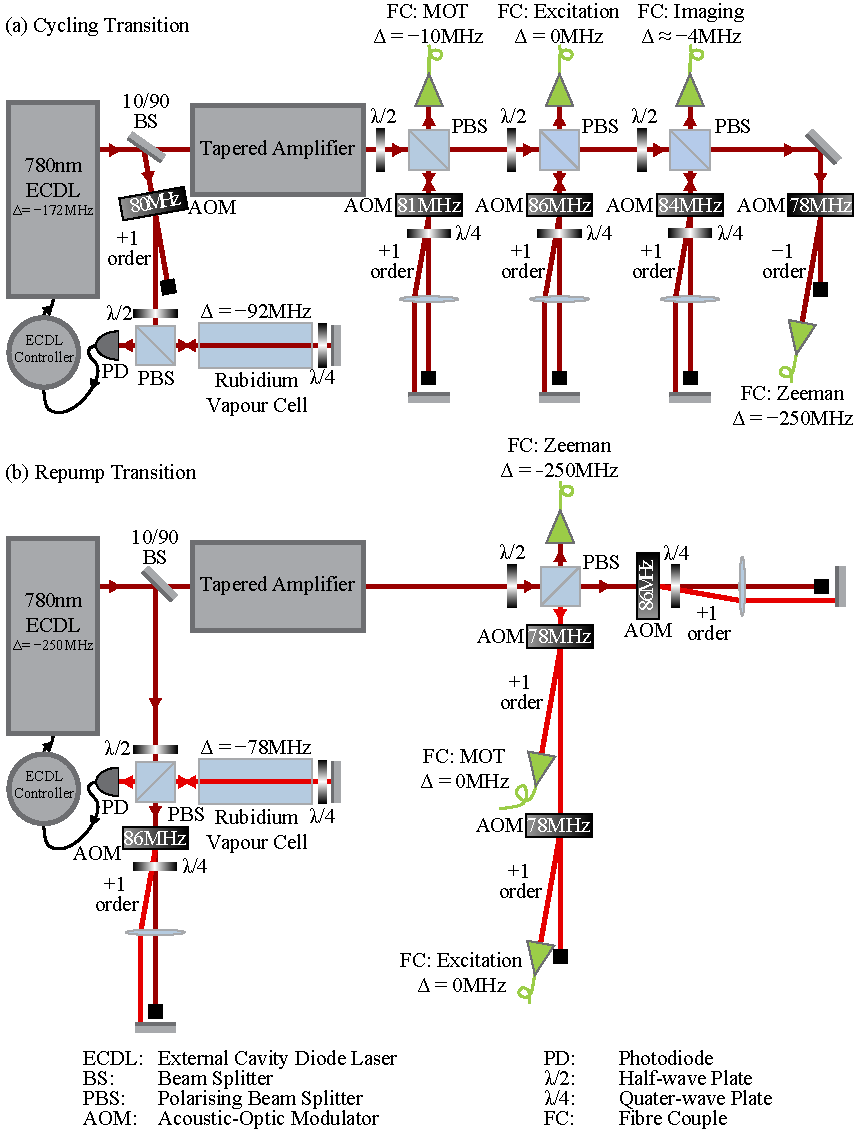
\includegraphics{part2/Figs/laser_setup.pdf}
    \caption{The simplified setup of the lasers locked to the rubidium-85 cycling (a) and repump (b) transitions.
    The \gls{ecdl} lasers are locked with saturated absorption spectroscopy, amplified with tapered amplifiers and offset for numerous applications using acousto-optic modulators.
    $\Delta$s refer to the frequency relative to the cycling or repump transitions.}
    \label{figure:laser_setup}
\end{figure}

\subsection{Rubidium Oven}
The source begins with an effusive Rubidium oven with a long heated collimation tube.
Typically effusive ovens are wasteful with large numbers of atoms lost into a large solid angles however this experimented makes use of a long heated collimation tube to collect and re-emit atoms that were initially emitted at high angles.
These atoms are re-emitted back to the reservoir or into the collimated atom beam leaving the collimation tube.
The rubidium reservoir was typically heated to \unit[80]{$^\circ$C} and the collimation tube to \unit[120]{$^\circ$C}.
A brief schematic of the oven can be found to the left in Figure~\ref{figure:zeemanoven} and more detail on the design, operation, and performance of the oven can be found in References~\cite{bell_slow_2010} and \cite{bell_cold_2011}.

\begin{figure}
    \center
    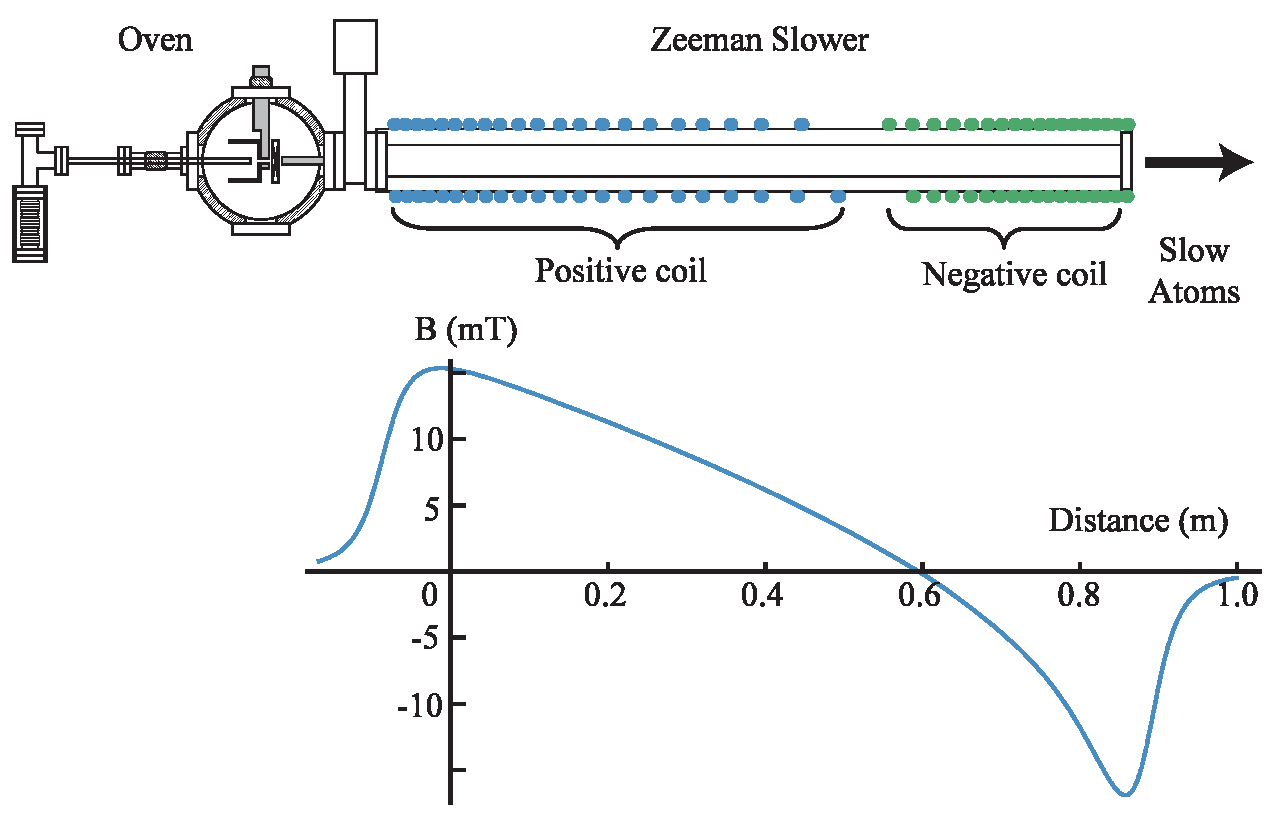
\includegraphics[width=145mm]{part2/Figs/ZeemanOven.pdf}
    \caption{A schematic of the rubidium atom source. Atomic vapour from the oven is directed into the Zeeman slower where a laser detuned from the atomic resonance (shown in red), in combination with a tapered magnetic coil (blue and green), with a magnetic field as shown, slows the thermal atoms.}
    \label{figure:zeemanoven}
\end{figure}

\subsection{Zeeman Slower}
Following the oven is the tapered pitch Zeeman slower which slows atoms down so that they can be captured by the trapping fields of \gls{mot}~\cite{bell_slow_2010}.
Zeeman slowers operate by using a laser red-detuned from resonance to slow the atoms down however as the atoms slow the conditions for resonance change due to the changing Doppler shift.
The solution to this quandrary used here is a tapered magnetic coil to apply a magnetic field to shift the atomic resonance such that a particular velocity class of atoms remains resonant with the light field, and thus is slowed, along the length of the Zeeman slower.
Atoms leaving the Zeeman slower typically had velocities around \unit[35]{m/s}, well within the capture velocity of the \gls{mot}.
A schematic of the Zeeman slower with along with the magnetic field produced by the tapered coil is shown in Figure~\ref{figure:zeemanoven}.

When extracting electrons from the \gls{mot} the magnetic coil must be turned off to prevent disruptions to the electron trajectory.

\subsection{Magneto-Optic Trap}
\Glspl{mot} use a combination of magnetic and light fields to trap and cool atoms to $\muup$K temperatures.
In the \gls{caeis} the \gls{mot} was formed from six counter propagating \unit[780]{nm} lasers in a a retro-reflective quasi-mirror \gls{mot} configuration~\cite{hanssen_using_2006,mcculloch_generation_2013} as shown in Figure~\ref{figure:mot} to allow for the accelerator structure consisting of transparent and reflective electrodes.
The static accelerating electric field was generated by two accelerator electrodes which were approximately \unit[11]{cm} in diameter and \unit[4]{mm} thick with the transmissive plate being \gls{ar} coated at \unit[780]{nm} and coated with indium-tin-oxide which is also transmisive to \unit[780]{nm} to 96\%.
The second reflective electrode was coposed of copper coated with polished gold and there was a third electrode that was not consistently used.
Each of the electrodes had an aperture in the center to allow the electron and ion bunches to pass through.
The magnetic component of the \gls{mot} was formed from two magnetic coils in an anti-Helmholtz configuration providing a zero-field region in the centre of the trap.

The \gls{mot} trapping lasers were detuned \unit[$-10$]{MHz} from the 5$^2$S$_{1/2} $(F=3) $\rightarrow$ 5$^2$P$_{3/2}$ (F$^\prime$=4) Rb85 transition and were mixed with on resonant 5S$_{1/2}$ (F=2) $\rightarrow$ 5P$_{3/2}$ (F$^\prime$=3) light to pump atoms that fell into the dark F=2 state.

\begin{figure}
    \center
    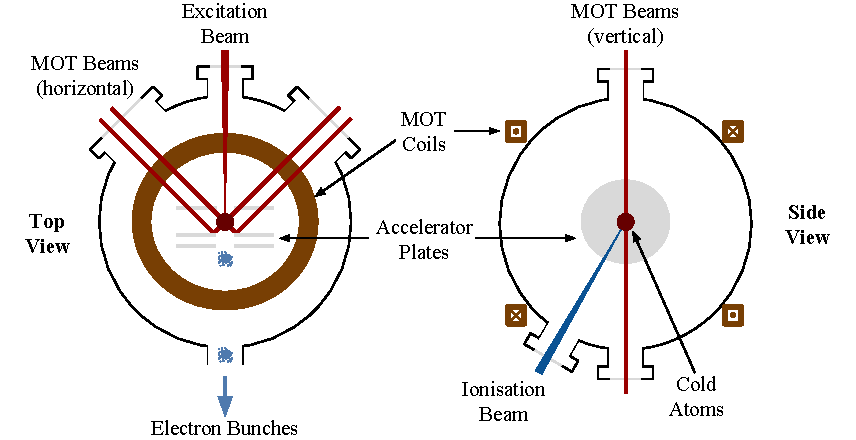
\includegraphics[width=145mm]{part2/Figs/MOTdiagram.pdf}
    \caption{A diagram of the magneto-optic trap, ionisation lasers and accelerator structures.}
    \label{figure:mot}
\end{figure}

\subsection{Ionisation}\label{section:two_stage_ionisation}

The \gls{caes} was capable of generating bunches of electron and ions with long (\unit[$\sim$10]{$\muup$s}), short (\unit[$\sim$5]{ns}), and ultrashort (\unit[$\sim$10]{ps}) bunch duration depending on the laser systems used~\cite{speirs_identification_2017,speirs_electron_2017}.
Depending on the ionisation pathway used, the \gls{caes} was able to produce cold bunches (\unit[$\sim$10]{K}) or hotter bunches (\unit[$>$10]{K}).
Generally cold electron bunches are preferable and bunch duration depends on the desired application, for example \gls{ued} requires ultrashort bunches.

Rubidium has a ground state ionisation threshold of \unit[4.18]{eV} which can be generated using a one blue and one red photon.
The \gls{caeis} has two options for the generation of blue light and two for red.
Red light could be generated by light from a \gls{cw} diode laser applified by a \gls{ta} and locked to the Rb85 5$^2$S$_{1/2} $(F=3) $\rightarrow$ 5$^2$P$_{3/2} $(F$^\prime$=4) cycling transition or it could be generated with a mode-locked Ti:sapphire amplified pulsed laser with a wavelength range of \unit[770]{nm} to \unit[830]{nm} and a minimum pulse length of \unit[35]{fs}.
Blue light could be generated with a tunable dye laser that produced \unit[460 to 490]{nm} light with a \gls{fwhm} duration of \unit[5]{nm} or with a \gls{cw} laser generated by a high-power tunable frequency-double diode laser.

Sequential ionisation utilised a single red photon to excite from the ground state to an intermediate excited state followed by a single blue photon to transition to a field-ionising state or to the ionisation continuum.
The bunch duration was determined by the shortest of; the duration of the laser pulse driving the transition from the exited state to the ionising state, the lifetime of the intermediate state, or by the depletion time of the intermediate state.

Multiphoton excitation happens when the laser intensities are high enough for nonlinear optical transitions to occur which was the case when the pulse lasers were tightly focused into the atom cloud.
In multiphoton excitation two or more photons are absorbed without transitioning via a real intermediate state.
If $n$ is the number of photon absorbed for the atom to reach its final ionised state then the transition rate is proportional to the $n$th power of the optical intensity~\cite{joachain_atoms_2011}.
Due to the short lifetime of the virtual intermediate states the bunch duration is determined by the duration of the laser pulses.
Multiphoton excitation can occur with just with photons of one colour or with two colour of photons.

Reonsance-enhanced multiphoton excitation occurs when a there is a combination of sequential excitation and multiphon excitation.
Here a number of photons are absorbed to excite the atom to a real intermediate state followed by more photon being absorbed to transition to the final state.
As less photons are required for each transision the overall transition rate can be much higher when compared to plain multiphoton excitation.

\begin{figure}
    \center
    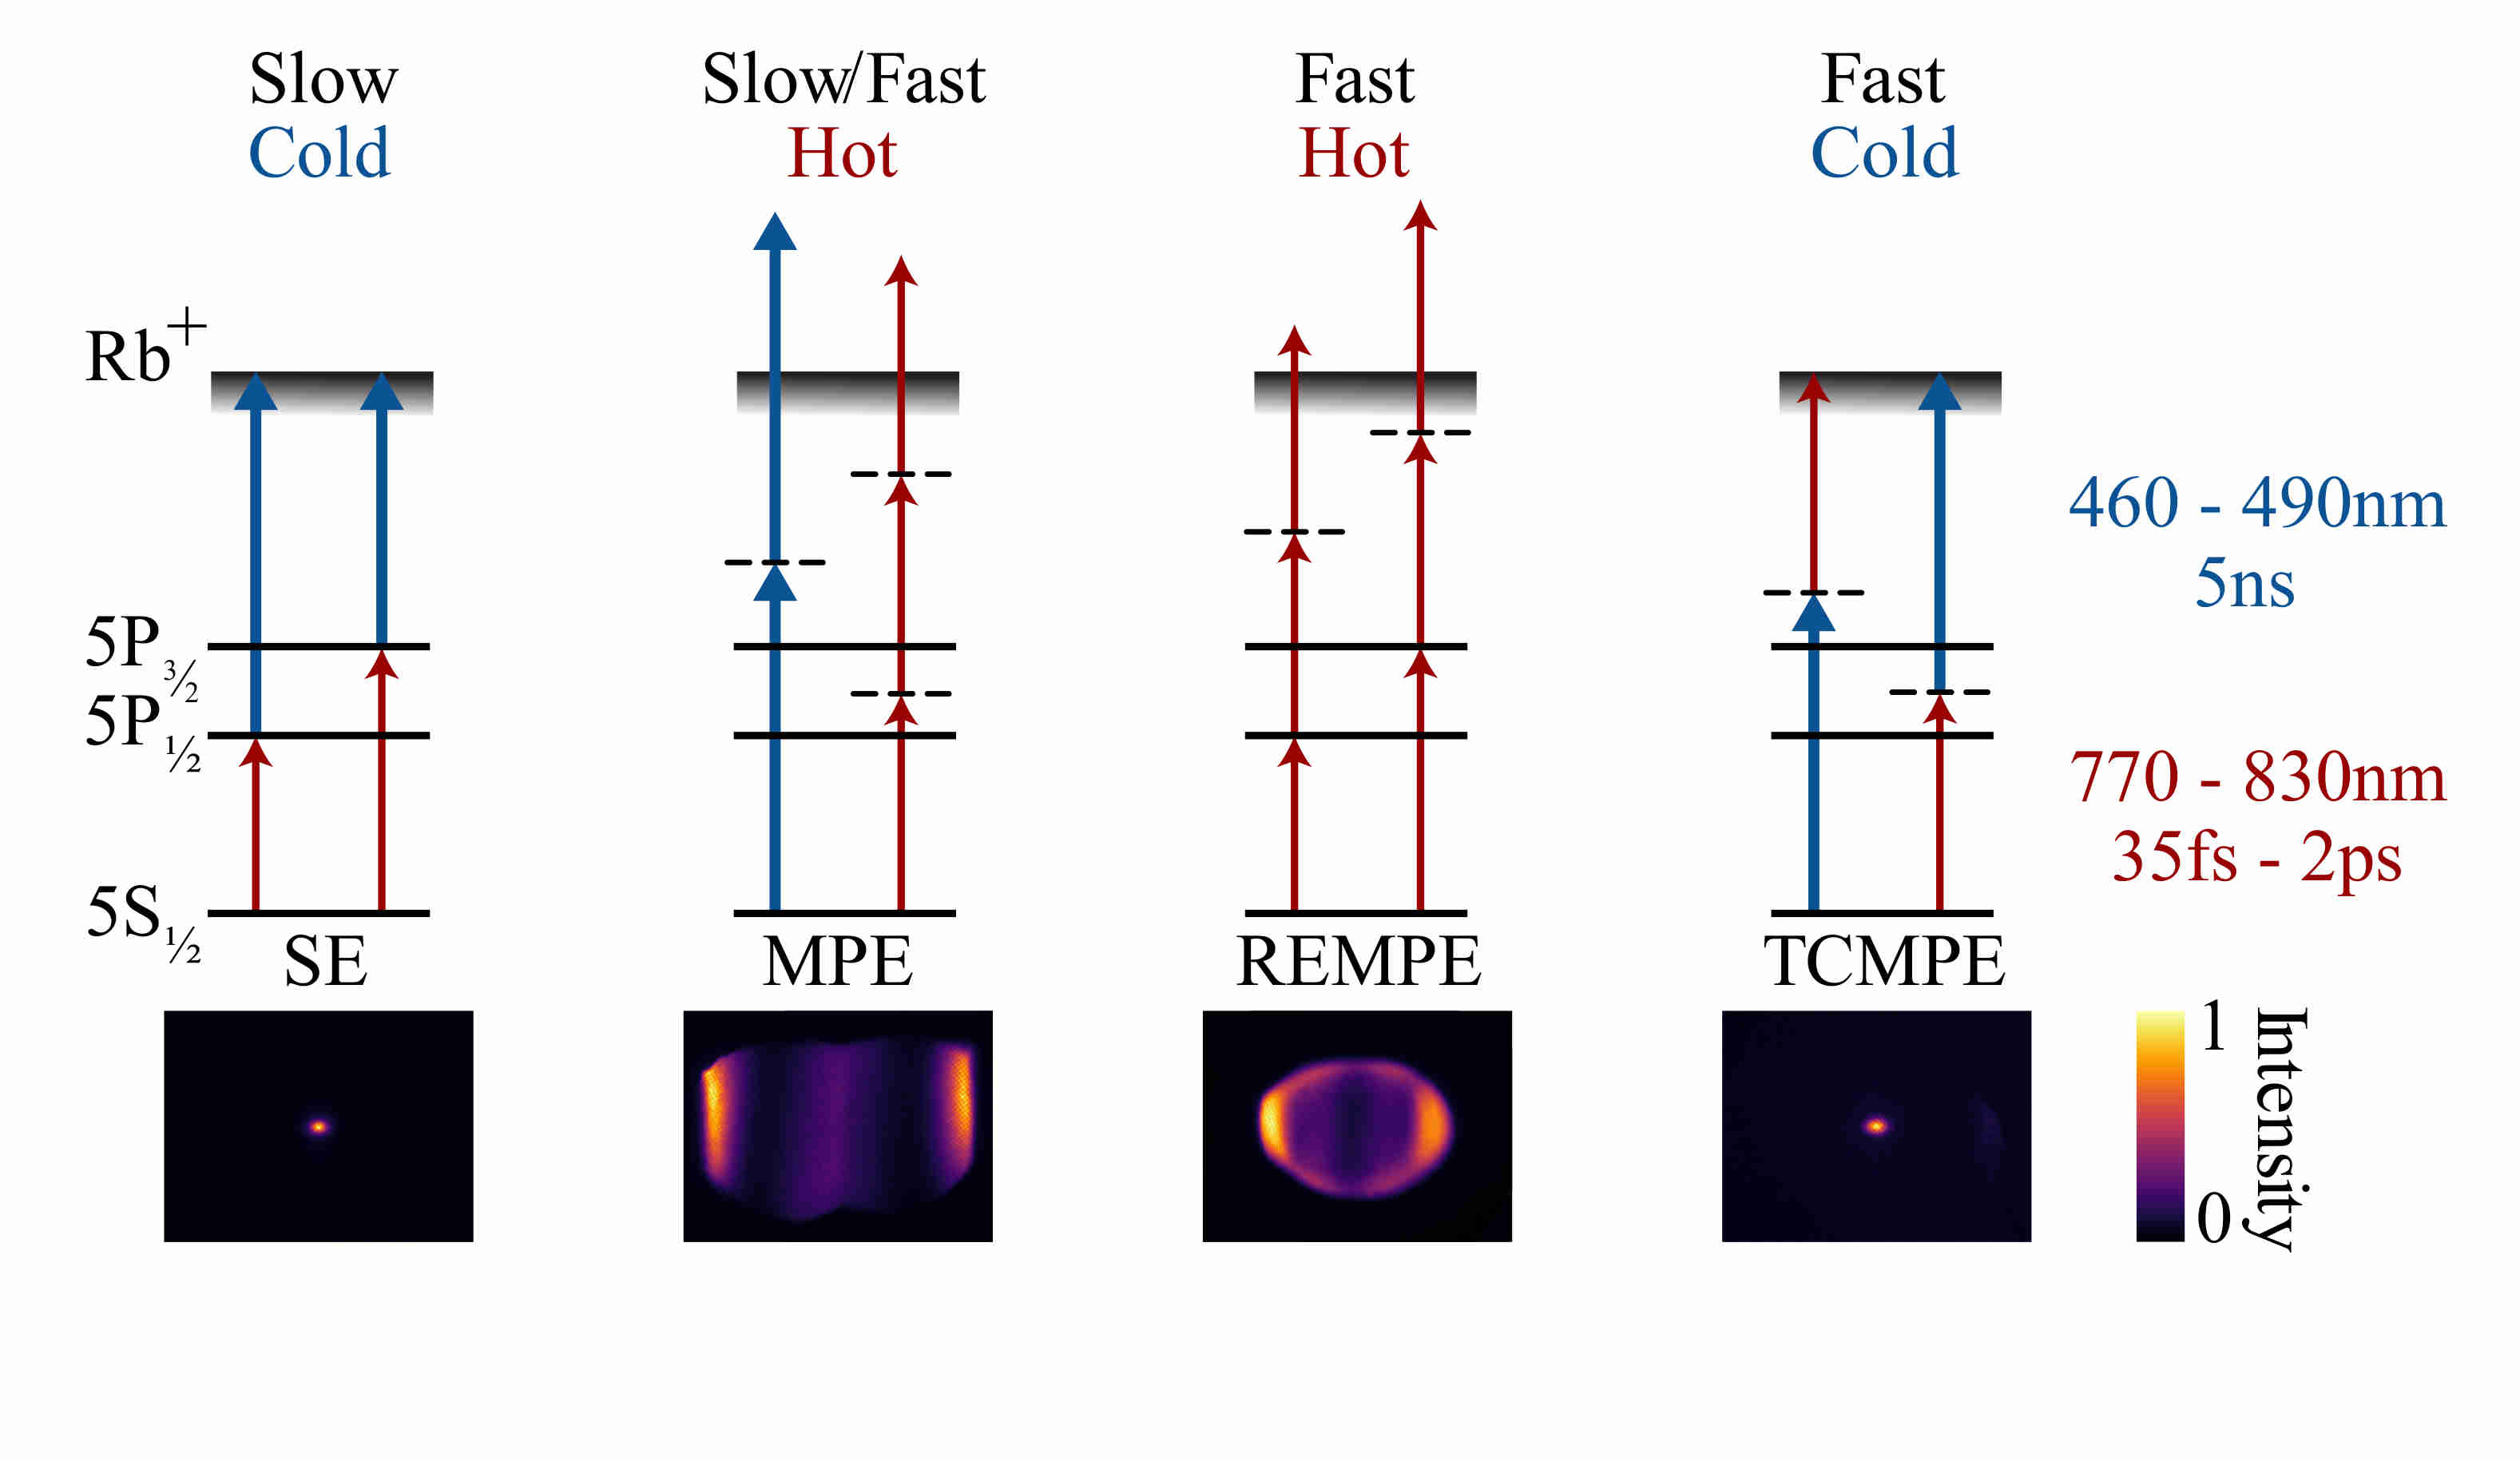
\includegraphics{part2/Figs/ionisationmodes.pdf}
    \caption{A number of photoexcitation pathways were possible in the presence of high intensity illumination by the red a blue lasers in the \gls{caes} such as sequential excitation (SE), multiphoton excitation (MPE), resonance-enhanced multiphoton excitation (REMPE), and two-colour multiphoton excitation (TCMPE). TCMPE is the only pathway that produces bunches that are cold and ultrashort. The images show the transverse momentum distributions for the detected bunches.}
    \label{figure:ionisation_modes}
\end{figure}

The temperature of particles generated from the \gls{caes} depends primarily on the excess ionisation energy given to the atoms by the absorbed photons.
Due to the complex orbits of electrons in high-lying states the relationship between absorbed photon energy and temperature is complex~\cite{mcculloch_high-coherence_2013} but it is generally true that with greater photon energy comes greater source temperature.
The classical ionisation threshold is lower in the presence of electric field, such as the accelerating field in the \gls{caeis}, due to the Stark-shift and the excess energy of an ion or electron relative to the classical ionisation threshold is:
\begin{equation}\label{equation:ionisation_energy_stark}
\Delta E = -E_I + 2\sqrt{ke^3F} + \sum_{i=0}^{n}{\frac{hc}{\lambda_i}},
\end{equation}
where $E_I=4.18\,meV$ is the ground state ionisation energy of rubidium-85, $k$ is the Coulomb constant, e is the elementary charge, $F$ is the strength of the electric field, $h$ is the Plank constant, and $c$ is speed of light.
The second term represent the Stark-shift of the classical ionisation threshold, and the last term is the sum of the energy of the $n$ photons involved in the ionisation, with wavelength $\lambda_i$.
Equation~\ref{equation:ionisation_energy_stark} assumes that rubidium is hydrogen-like which is a good approximation as long as $E_I \gg 2\sqrt{ke^3F}$.

Sequential excitation and two-colour multiphoton excitation are the only ionisation processing that producce cold electrons as the excess ionisation energy is minised by tuning the photon energy.
This can be seen in Figure~\ref{figure:ionisation_modes} in the momentum distributions.

Due to the tunability of the lasers involved in generating cold electrons the it was possible to directly ionise regardless of the electric field which resulted in short duration bunches, field-ionise such that the majority of the bunch had a short duration but some particles continued to tunnel out over a longer duration, or to excite the atoms such that tunneling through the Stark-shifted potential was the only route to ionisation resulting in lower bunch current and long duration.
The short bunch duration depended on the duration of the laser pulses, generally either the ultrafast bunches with less than \unit[320]{ps} duration using the red femtosecond pulse laser, or \unit[5]{ns} long bunches with \gls{cw} red and the \unit[5]{ns} pulsed blue laser.
Long duration bunch length depended on the lifetime of the atomic states involved and tended to be of order \unit[10]{$\muup$s}~\cite{speirs_identification_2017}.

\subsubsection{Beam Shaping}

The \glspl{caeis} was able to shape the profile of the electron and ion bunches produced by manipulating the red excitation and blue ionisation beam~\cite{mcculloch_arbitrarily_2011}.
The lasers imparted their profiles onto the ionised atoms which, for cold low-emittance bunches, could be maintained to the detector.
The transverse bunch profile was determined by the red exciation laser profile combined with the density profile of the atomic cloud.
Similarly the longitudinal profile depended on the ionisation laser profile and atomic cloud density.

Control over the excitation beam profile was achieved with a \gls{slm} and an interative feedback system~\cite{van_bijnen_patterned_2015} and with a second \gls{slm} and control system the longidutinal profile would be controllable.
A schematic of the bunch profile system is shown in Figure~\ref{figure:beam_shaping_schematic} and an example of its performance can be seen in Figure~\ref{figure:beam_shaping}.

\begin{figure}
    \center
    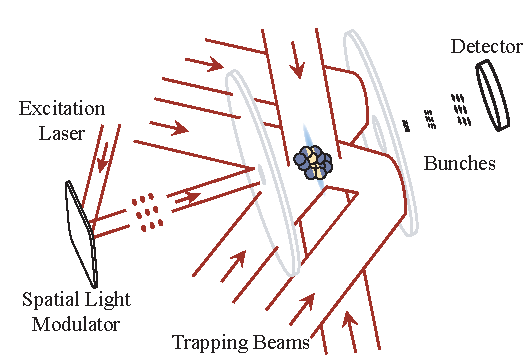
\includegraphics{part2/Figs/beam_shaping_schem.pdf}
    \caption{A schematic of the shaping apparatus. The excitation laser pulse is shaped with a \gls{slm} to form an arbitrary beam profile at the atom cloud, imparting that profile onto the bunch produced by the \gls{caeis}. In this diagram the blue ionisation laser comes from behind the atom cloud.}
    \label{figure:beam_shaping_schematic}
\end{figure}

\begin{figure}
    \center
    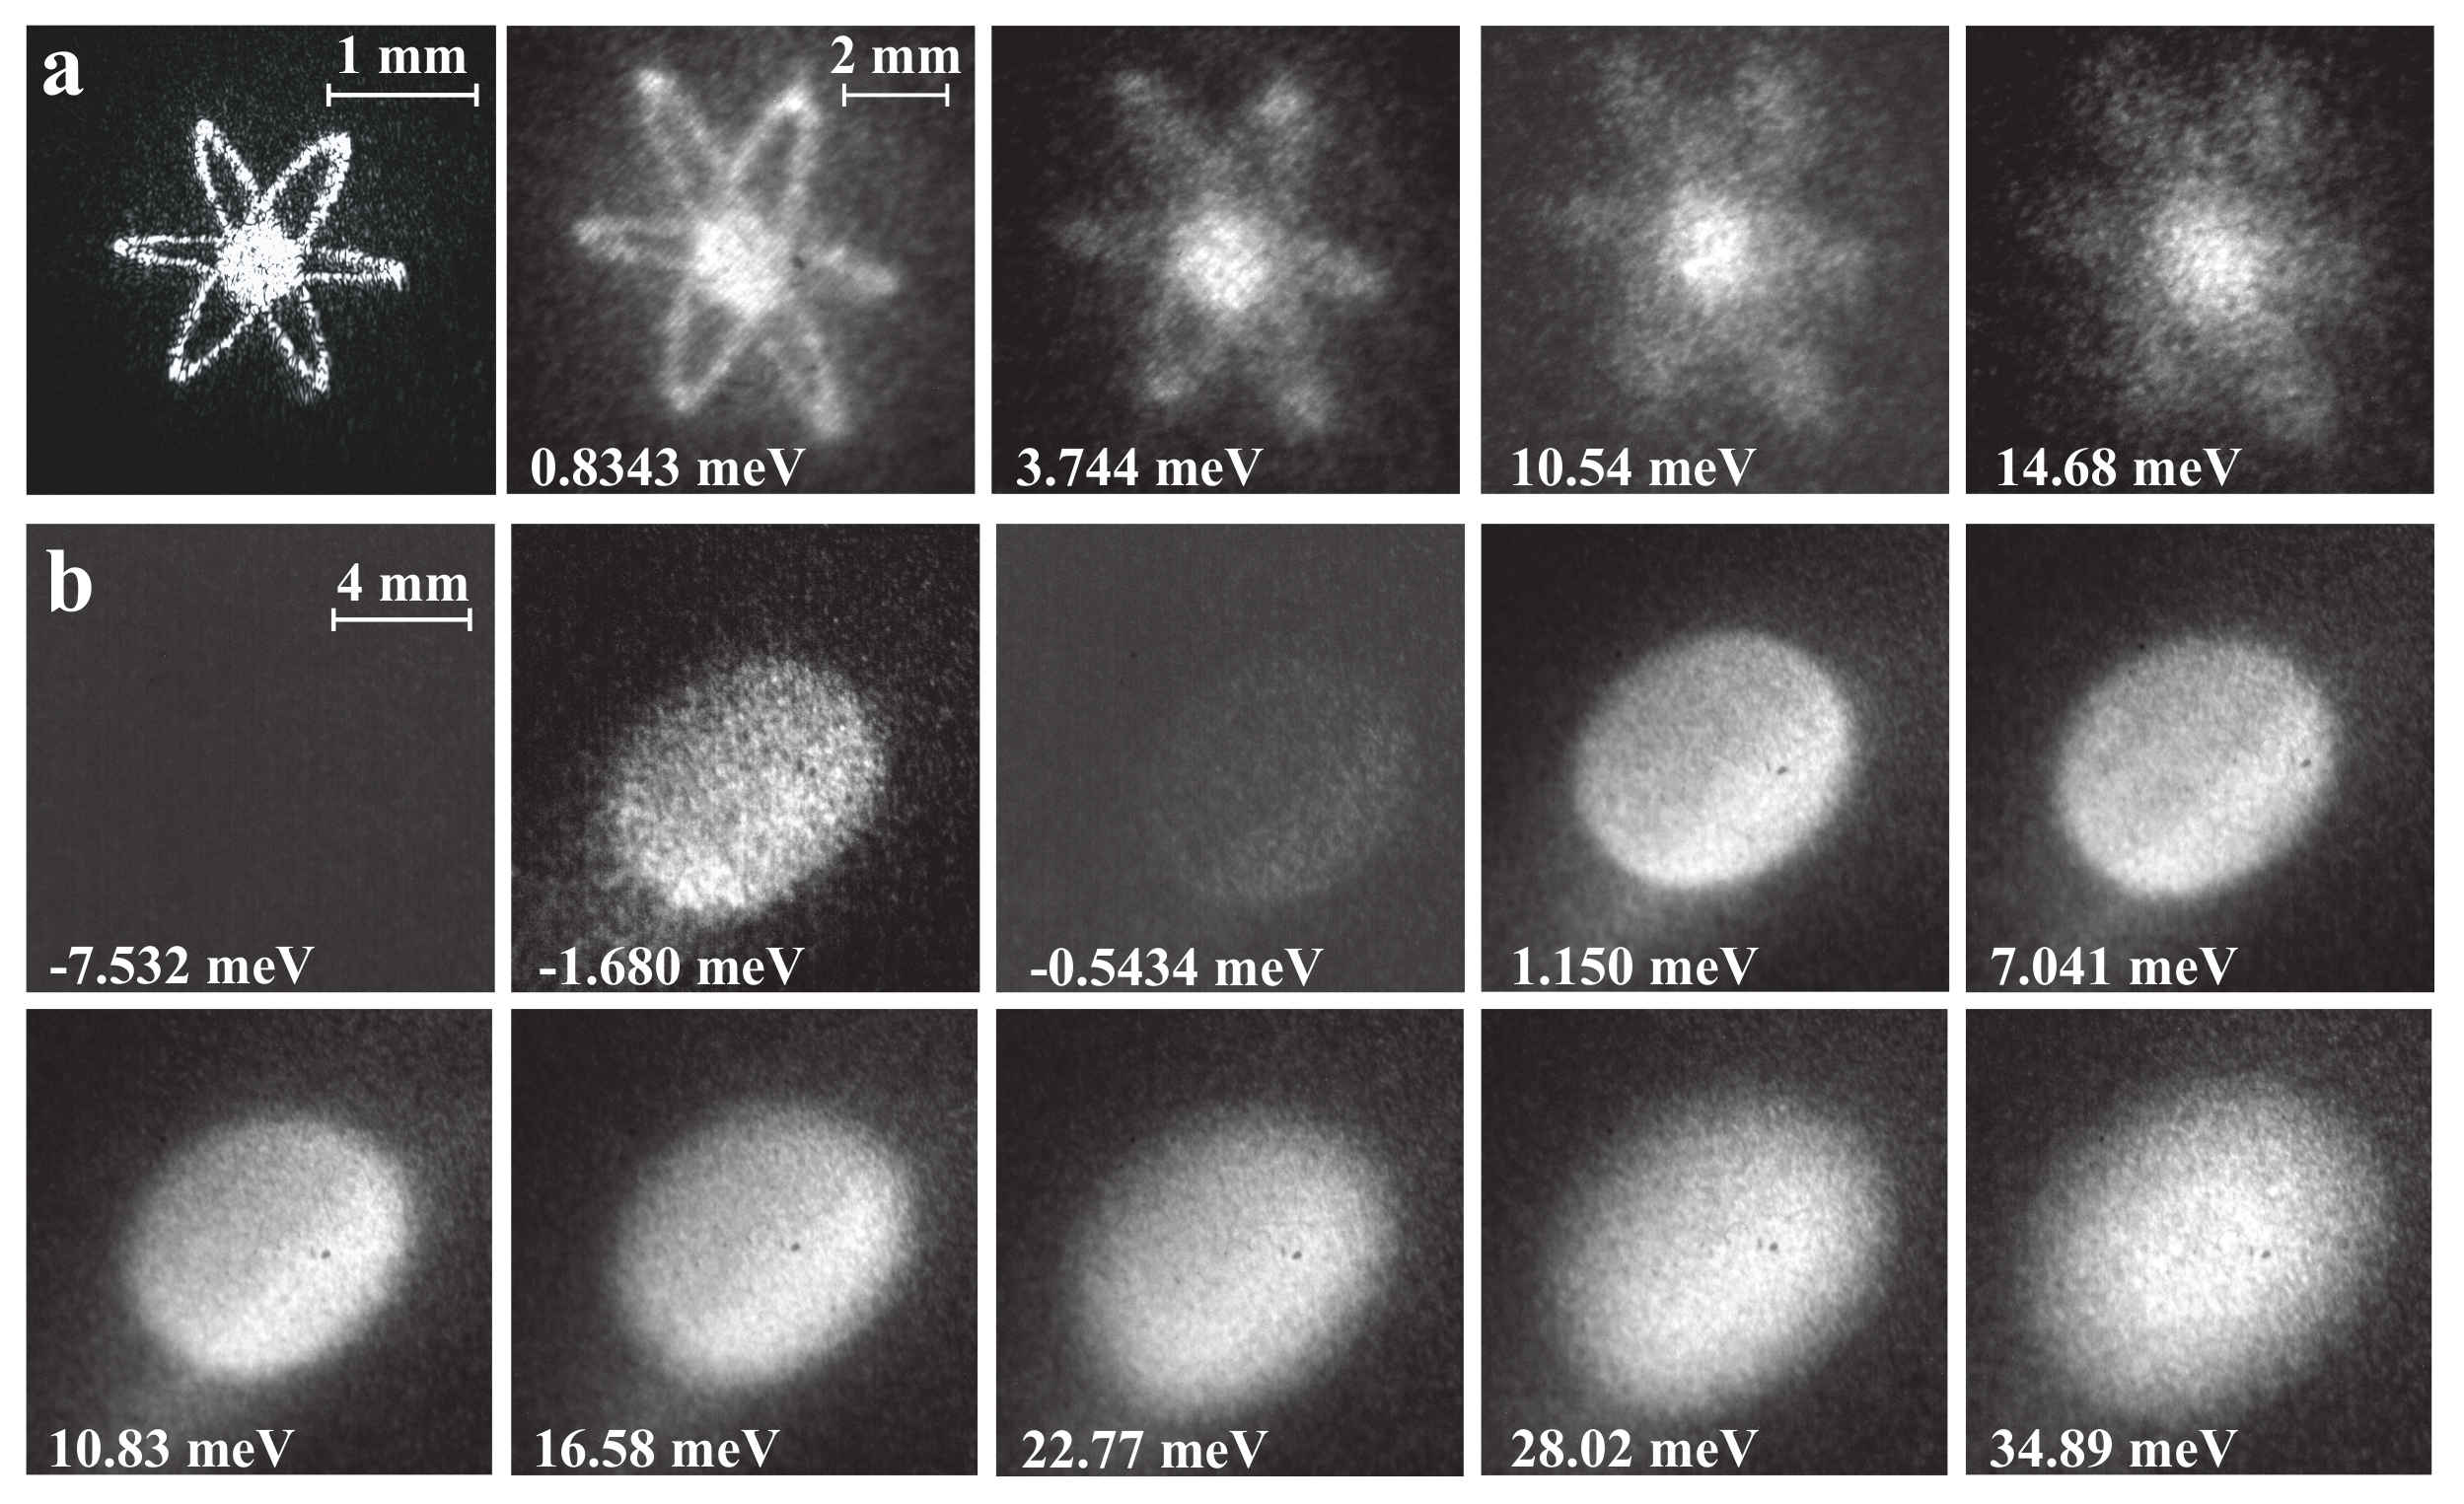
\includegraphics{part2/Figs/beam_shaping.pdf}
    \caption{An example of beam shaping and the effects of temperature on the degradation of the bunch profile.
    \emph{a} Excitation laser profile (left), followed by detected electron bunches as excess ionisation energy is varied.
    \emph{b} Electron bunches genearted from a uniform excitation laser profile as excess energy is varied.
    At \unit[-1.680]{meV} bunch current increases as the ionisation laser couples to a Rydberg state.}
    \label{figure:beam_shaping}
\end{figure}

Control over the bunch profile allows for customisation and feedback for whatever application the \gls{caeis} is being used for but is of particular interest for countering space-charge expansion.
With the bunch charges achieved to date only the ultrashort duration bunches are dense enough to experience significant space-charge expansion which degrades the coherence and emittance of the beam and is thus detrimental to imaging applications.
Suppression of space-charge expansion has been demonstrated with the \gls{caeis} by beam shaping~\cite{luiten_how_2004,thompson_suppression_2016}.

\subsection{Beam Optics}

There were a number of systems in place for manipulating the electron and ion beams; a solenoid lens, an Einzel lens, a magnetic quadrupole lens, a one-axis deflector, and a number of permanent magnets located outside the vaccum system.
The lenses were used to focus the bunches, usually to a focus on the detector but sometimes to manipulate the size of the beam at the sample plane.
The quadrupole lens was used to counter astigmatism in the beam and is discussed in more detail in Section~\ref{section:quadrupole}.
The deflector was located after the sample stage and was used to streak bunches across the detector.
The permanent magnets were used to steer electron bunches through the system, through a number of apertures and countering the deflection imposed by a number of anomalous magnetic fields present with the \gls{caeis}.

\subsection{Sample Management}

Experimental samples were mounted on a custom sample mount formed from an alumium paddle that was large enough to mount eight \gls{tem} samples and block any portion of the beam not passing through the samples.
The samples were held by two commercial \gls{tem} mounts attached to the paddle that were able to fit \unit[3.05]{mm} diamter samples with approximately \unit[2]{mm} diameter of the sample visible to the bunches when the sample lid was in place.
Grazing indicence reflection diffraction samples could also be mounted at the end of the paddle as shown in Figure~\ref{figure:sample_holder}.
The sample paddle was mounted on a stage with manual control over two-axis translation transverse to the beam axis and rotation.
The sample paddle could also be connect to a high-voltage supply to allow for the sample to be bias to further manipulate the beam energy as described in Secion~\ref{section:sample_bias}.

\begin{figure}
    \centering
    \begin{subfigure}{0.49\linewidth}
    \centering
    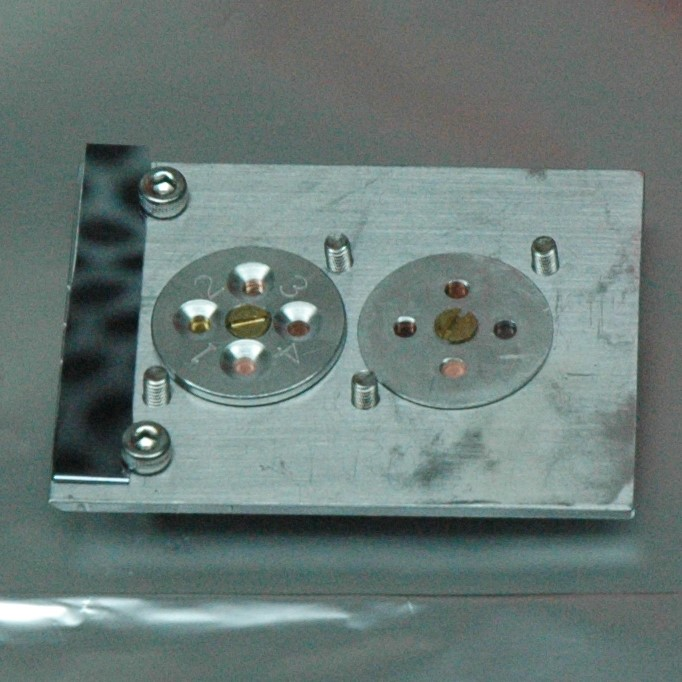
\includegraphics[width=\linewidth]{part2/Figs/sample_holder_alone.jpg}
    \end{subfigure}
    \begin{subfigure}{0.49\linewidth}
    \centering
    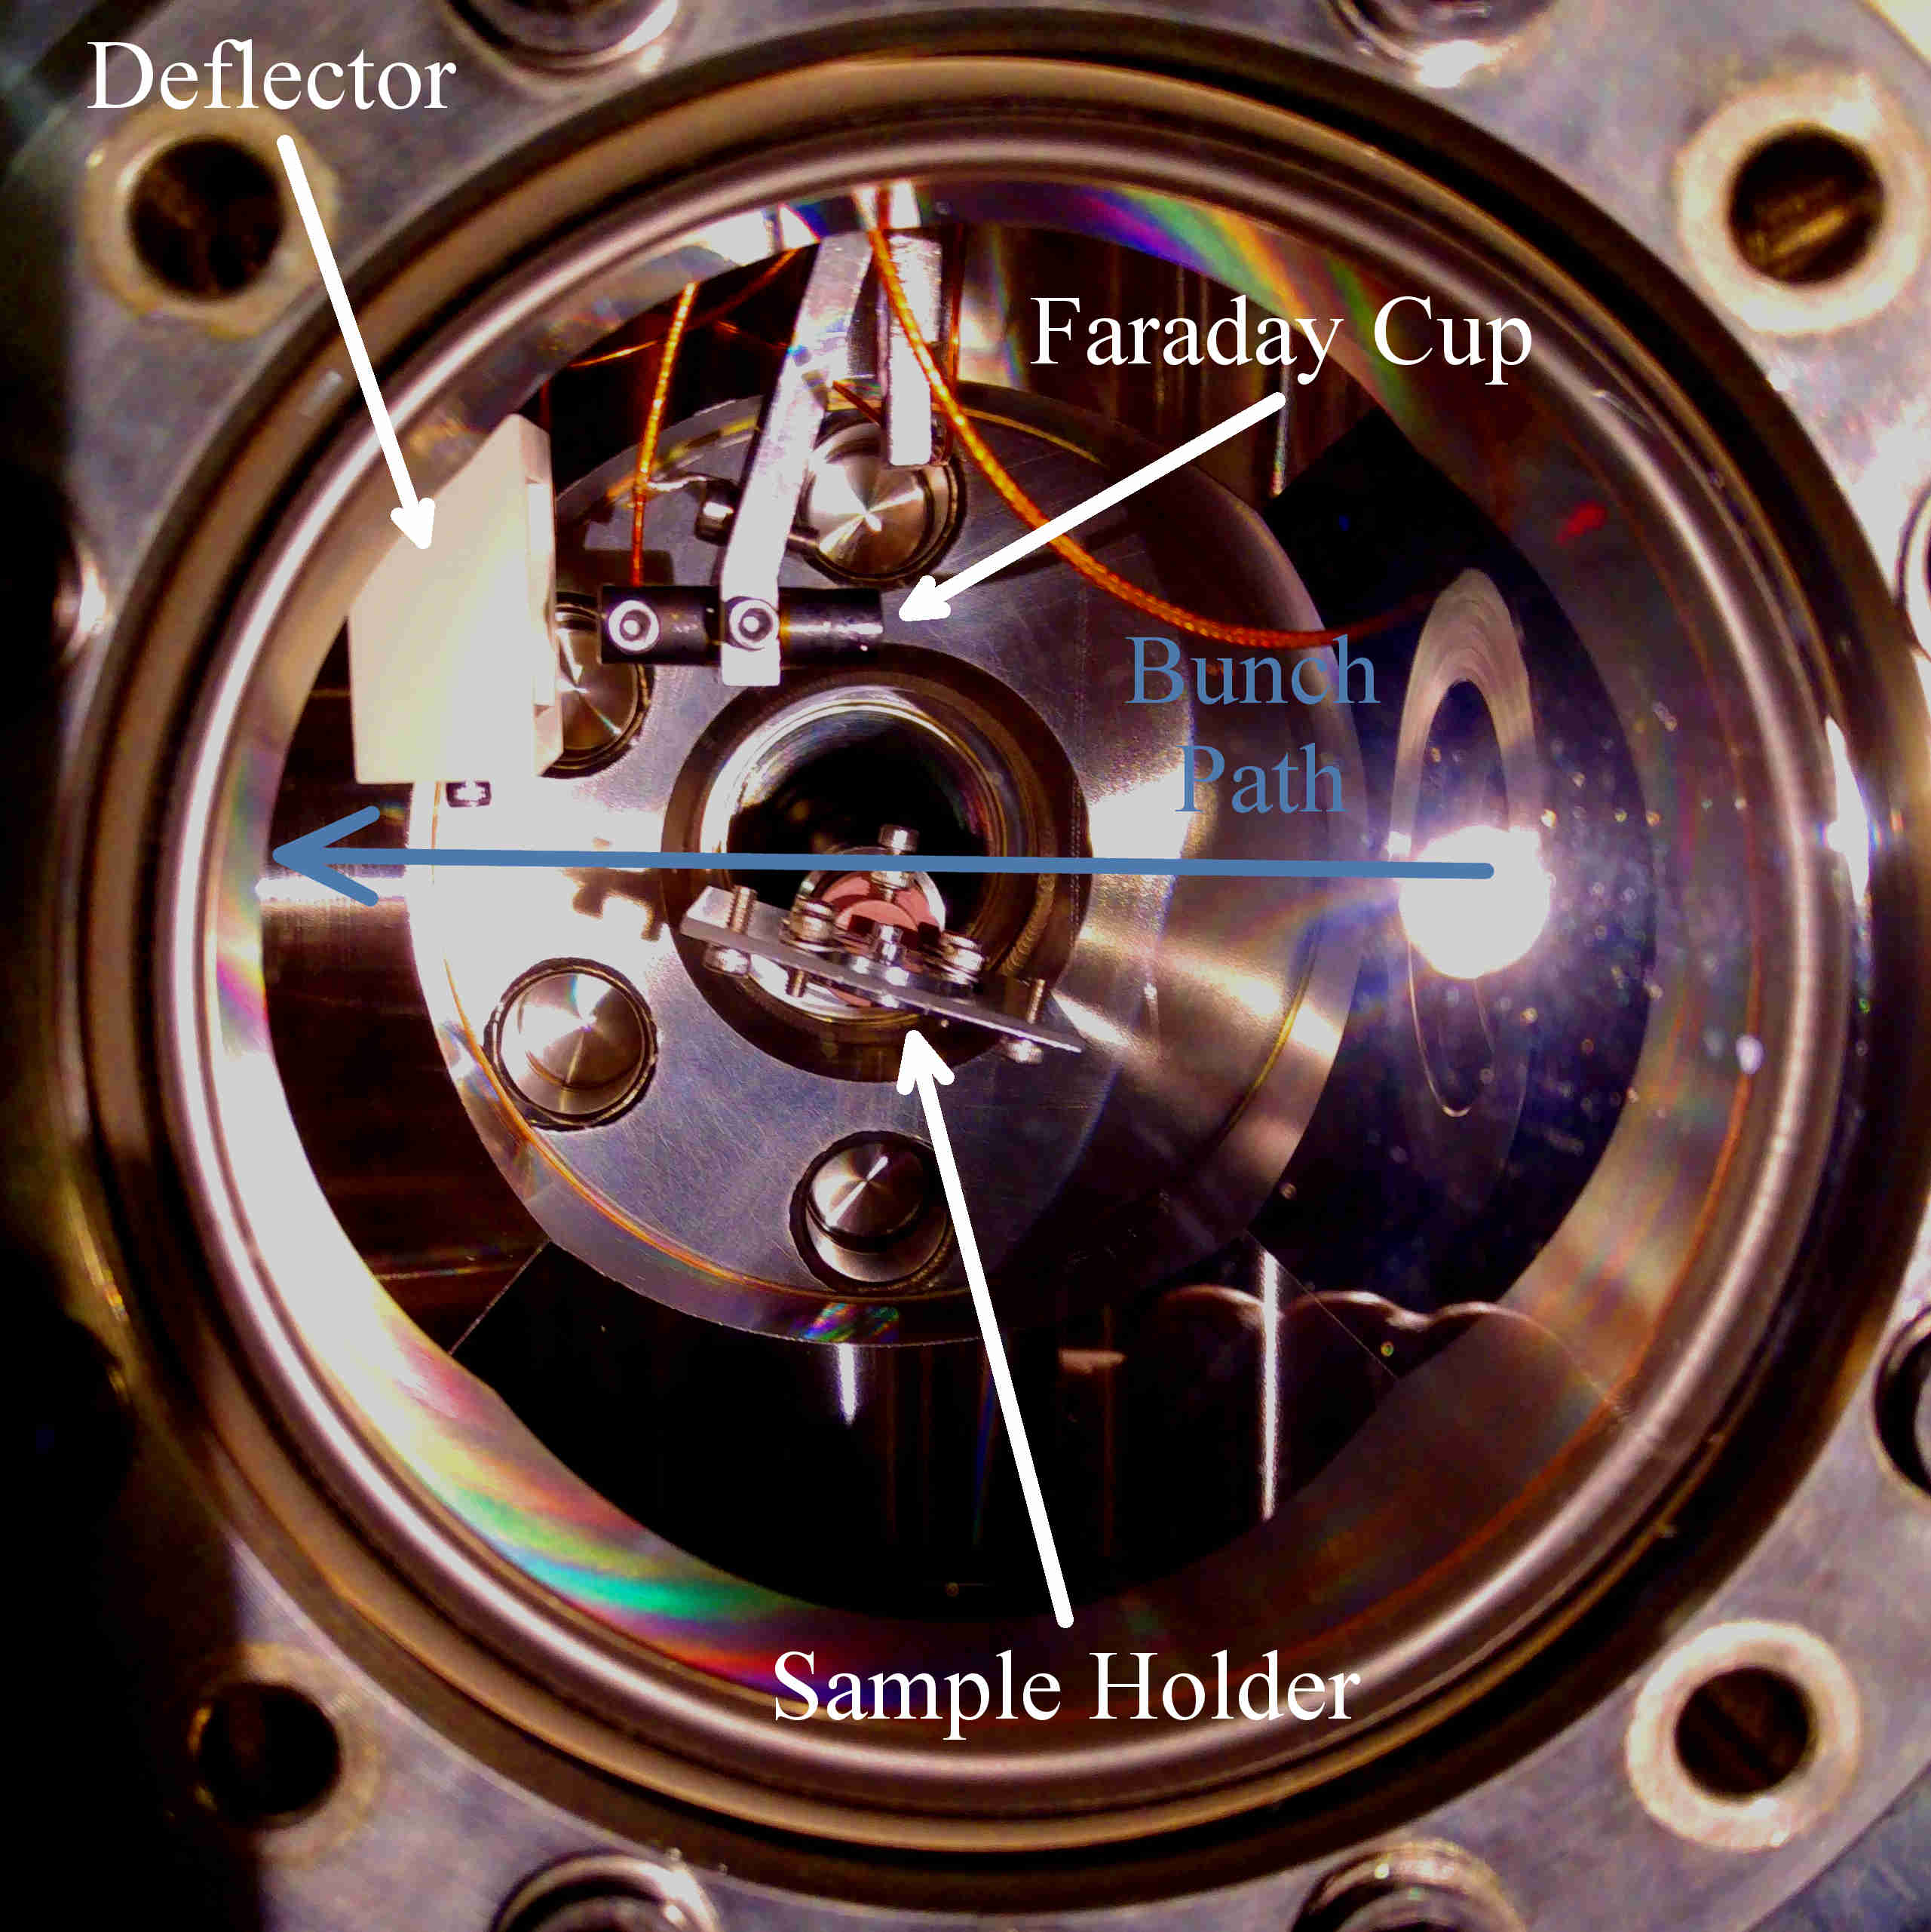
\includegraphics[width=\linewidth]{part2/Figs/sample_holder_in_vitro.jpg}
    \end{subfigure}
    \caption{The sample holder used in the \gls{caes}. In the left photograph the sample holder with eight transmission samples and a relection sample is shown. On the right is the sample holder in the sample chamber, with the post-sample deflector and Faraday cup also visible retracted from the beam path (bunches travel from right to left).}
    \label{figure:sample_holder}
\end{figure}

\subsection{Timing}\label{section:pulse_blaster}

Synchronisation throughout the experiment was achieved with a 24-channel digital timing card\footnote{Spincore Pulseblaster PCI mounted in external USB enclosure.}.
Low voltage TTL signals are used signal to the numerous devices involved in timing of the experiment.
The \gls{caeis} operated at the frequency of the flashlamp of the \unit[5]{ns} blue pulse laser, \unit[10]{Hz}.
The sequency began with \gls{mot} and Zeeman lasers and fields turning on to load the trap for approximately \unit[90]{ms}.
The trapping lasers and fields were extinguisted \unit[5]{ms} before the excitation and ionisation lasers and \gls{ccd} camera were triggered to generate and detect the electron or ion bunch.

\section{Current Limitations}

There were a number of factors preventing the \gls{caeis} achieving its goal of single-shot ultrafast electron diffractive imaging, namely electron flux and beam stability.
These factors also require improvement for other \gls{caes} goals such as \gls{fib} milling, and general electron and ion imaging.

The minimum electron flux required for \gls{ued} is 10$^6$ electrons per bunch~\cite{van_oudheusden_compression_2010} whereas this iteration of the \gls{caes} was only able to get $5\times10^5$ electrons.
There are a few avenues available to the \gls{caeis} to improve the bunch count such as increasing the \gls{mot} density, increasing the power of the ionisation laser, better optimisation of the ionisation pathways~\cite{mcculloch_field_2017}, and running the apparatus in \gls{cw} mode.
\Gls{cw} mode  has the potential to increase the number of particals per second however some applications would be difficult or impossible without discrete bunches.
An investigation of the performance of the apparatus in \gls{cw} mode is shown in Section\ref{section:pulse_vs_continuous}.

The stability of the source was also problematic, particularly for electron bunches, as a number of transient effects interferred with the path of the beams on a shot-to-shot and minute-to-minute timescale.
Effects such as eddy currents due to the switching of the strgon magnetic fields in the steel of the vaccum system and boards the optics are mounted on was one of the primary suspects for a source of the perturbations in the beam path.
Other potential sources are the electronic equipment such as power supplies and switches that were placed as far away from the beam path as practical but were still in the vicinity.
The poor stability of the source made some measurements difficult and other impossible.
Multi-shot measurements were required in a number of cases and, due to the drift of the beam, straight averages of the images from the detector resulted in a unusable blur.
Generating usable images for multi-shot measurements required `registration' of the images, set averages where the features in each individual image was aligned with the other images to prevent blurring.
Measurements without sharp features could not be well registered, as the registration algorithms have trouble precisly aligning the images.
Registration is discussed further in Section~\ref{section:registration}.

\section{Pulsed vs Continuous}\label{section:pulse_vs_continuous}
Comparing the performance of the source in its usual pulse mode against the performance as a continuous source had the potential to show pathways for improving the pulsed mode as well as a mode that would provide better performance for particular applications, as some measurements, such as simple \gls{cdi}, do not require the source to be pulsed.
Continous mode functions by using the two-stage ionisation and acceleration on the Zeeman slowed atom beam from the oven without further cooling and trapping in the \gls{mot}.
It was hoped that the beam current would increase with this mode of operation and that the beam produced would be subject to less trajectory perturbation as the magntic fields were not switching.

While the entire apparatus and control system had been designed to operate in pulse mode it was fortunately relatively simple to modify the setup to operate continuously.
The \gls{mot} was disabled, the excitation beam was left on, and the \gls{cw} blue was used instead of the usual blue pulse laser to act as the ionisation laser.

Before switching to continuous mode the \gls{caeis} had been measured to have \unit[$0.42\times10^6$]{electrons per bunch} equating to a beam current of \unit[$4.2\times10^6$]{electrons per second}.
Initially the continuous mode was producing \unit[$0.64\times10^6$]{electrons per second} however there were a number of optimisations available to improve the current, as detailed below.

\subsection{Oven Temperature to Electron Count}
When operating in pulsed mode the \gls{mot} was given more than enough time to saturate and thus there was no benefit to producing more electrons from the oven.
In continuous mode the beam current was dependent on the density of atoms in the ionisation region which could be increased by producing more atoms from the oven.

The atomic flux from the oven could easily be increased by running the oven at a higher temperature.
During normal operation the oven was set to a temperature of approximately \unit[80]{$^\circ$C} (rubidium has a melting point of \unit[39.30]{$^\circ$C}) however the oven is able to operate at up to \unit[200]{$^\circ$C}.

{\color{red}Atomic flux from oven vs temperature??}

The effects of the oven temperature on the beam current are shown in Figure~\ref{figure:oven_counts}.
There was a significant increase in the beam current as the oven temperature was increased, with a high enough temperature is was even greater than that of the pulsed mode bunches.
The unfortunate side affect of running the oven at such high temperatures is that the lifetime of the \unit[5]{g} rubidium ampule in the oven will be drastically reduced to the point where a threefold increase in current is not worth the reduced lifetime.
This data indicates that the \gls{cw} beam current could be improved with the use of transverse compression of the atom beam which would provide a similar improvement to beam current as more atoms would be present in the ionisation region.

\begin{figure}
    \center
    %% Creator: Matplotlib, PGF backend
%%
%% To include the figure in your LaTeX document, write
%%   \input{<filename>.pgf}
%%
%% Make sure the required packages are loaded in your preamble
%%   \usepackage{pgf}
%%
%% Figures using additional raster images can only be included by \input if
%% they are in the same directory as the main LaTeX file. For loading figures
%% from other directories you can use the `import` package
%%   \usepackage{import}
%% and then include the figures with
%%   \import{<path to file>}{<filename>.pgf}
%%
%% Matplotlib used the following preamble
%%
\begingroup%
\makeatletter%
\begin{pgfpicture}%
\pgfpathrectangle{\pgfpointorigin}{\pgfqpoint{4.282500in}{2.141250in}}%
\pgfusepath{use as bounding box, clip}%
\begin{pgfscope}%
\pgfsetbuttcap%
\pgfsetmiterjoin%
\definecolor{currentfill}{rgb}{1.000000,1.000000,1.000000}%
\pgfsetfillcolor{currentfill}%
\pgfsetlinewidth{0.000000pt}%
\definecolor{currentstroke}{rgb}{1.000000,1.000000,1.000000}%
\pgfsetstrokecolor{currentstroke}%
\pgfsetdash{}{0pt}%
\pgfpathmoveto{\pgfqpoint{0.000000in}{0.000000in}}%
\pgfpathlineto{\pgfqpoint{4.282500in}{0.000000in}}%
\pgfpathlineto{\pgfqpoint{4.282500in}{2.141250in}}%
\pgfpathlineto{\pgfqpoint{0.000000in}{2.141250in}}%
\pgfpathclose%
\pgfusepath{fill}%
\end{pgfscope}%
\begin{pgfscope}%
\pgfsetbuttcap%
\pgfsetmiterjoin%
\definecolor{currentfill}{rgb}{1.000000,1.000000,1.000000}%
\pgfsetfillcolor{currentfill}%
\pgfsetlinewidth{0.000000pt}%
\definecolor{currentstroke}{rgb}{0.000000,0.000000,0.000000}%
\pgfsetstrokecolor{currentstroke}%
\pgfsetstrokeopacity{0.000000}%
\pgfsetdash{}{0pt}%
\pgfpathmoveto{\pgfqpoint{0.691823in}{0.532919in}}%
\pgfpathlineto{\pgfqpoint{4.028722in}{0.532919in}}%
\pgfpathlineto{\pgfqpoint{4.028722in}{1.926770in}}%
\pgfpathlineto{\pgfqpoint{0.691823in}{1.926770in}}%
\pgfpathclose%
\pgfusepath{fill}%
\end{pgfscope}%
\begin{pgfscope}%
\pgfpathrectangle{\pgfqpoint{0.691823in}{0.532919in}}{\pgfqpoint{3.336899in}{1.393852in}} %
\pgfusepath{clip}%
\pgfsetrectcap%
\pgfsetroundjoin%
\pgfsetlinewidth{1.003750pt}%
\definecolor{currentstroke}{rgb}{0.309804,0.478431,0.682353}%
\pgfsetstrokecolor{currentstroke}%
\pgfsetdash{}{0pt}%
\pgfpathmoveto{\pgfqpoint{1.029684in}{0.596936in}}%
\pgfpathlineto{\pgfqpoint{1.584443in}{0.629190in}}%
\pgfpathlineto{\pgfqpoint{2.270593in}{0.845827in}}%
\pgfpathlineto{\pgfqpoint{2.650166in}{1.273641in}}%
\pgfpathlineto{\pgfqpoint{2.825353in}{1.276714in}}%
\pgfpathlineto{\pgfqpoint{3.238294in}{1.418479in}}%
\pgfpathlineto{\pgfqpoint{3.667920in}{1.479532in}}%
\pgfpathlineto{\pgfqpoint{3.903588in}{1.780648in}}%
\pgfusepath{stroke}%
\end{pgfscope}%
\begin{pgfscope}%
\pgfpathrectangle{\pgfqpoint{0.691823in}{0.532919in}}{\pgfqpoint{3.336899in}{1.393852in}} %
\pgfusepath{clip}%
\pgfsetbuttcap%
\pgfsetroundjoin%
\pgfsetlinewidth{1.003750pt}%
\definecolor{currentstroke}{rgb}{0.000000,0.000000,0.000000}%
\pgfsetstrokecolor{currentstroke}%
\pgfsetdash{{6.000000pt}{6.000000pt}}{0.000000pt}%
\pgfpathmoveto{\pgfqpoint{0.691823in}{0.951074in}}%
\pgfpathlineto{\pgfqpoint{4.028722in}{0.951074in}}%
\pgfusepath{stroke}%
\end{pgfscope}%
\begin{pgfscope}%
\pgfsetrectcap%
\pgfsetmiterjoin%
\pgfsetlinewidth{1.003750pt}%
\definecolor{currentstroke}{rgb}{0.000000,0.000000,0.000000}%
\pgfsetstrokecolor{currentstroke}%
\pgfsetdash{}{0pt}%
\pgfpathmoveto{\pgfqpoint{4.028722in}{0.532919in}}%
\pgfpathlineto{\pgfqpoint{4.028722in}{1.926770in}}%
\pgfusepath{stroke}%
\end{pgfscope}%
\begin{pgfscope}%
\pgfsetrectcap%
\pgfsetmiterjoin%
\pgfsetlinewidth{1.003750pt}%
\definecolor{currentstroke}{rgb}{0.000000,0.000000,0.000000}%
\pgfsetstrokecolor{currentstroke}%
\pgfsetdash{}{0pt}%
\pgfpathmoveto{\pgfqpoint{0.691823in}{0.532919in}}%
\pgfpathlineto{\pgfqpoint{0.691823in}{1.926770in}}%
\pgfusepath{stroke}%
\end{pgfscope}%
\begin{pgfscope}%
\pgfsetrectcap%
\pgfsetmiterjoin%
\pgfsetlinewidth{1.003750pt}%
\definecolor{currentstroke}{rgb}{0.000000,0.000000,0.000000}%
\pgfsetstrokecolor{currentstroke}%
\pgfsetdash{}{0pt}%
\pgfpathmoveto{\pgfqpoint{0.691823in}{1.926770in}}%
\pgfpathlineto{\pgfqpoint{4.028722in}{1.926770in}}%
\pgfusepath{stroke}%
\end{pgfscope}%
\begin{pgfscope}%
\pgfsetrectcap%
\pgfsetmiterjoin%
\pgfsetlinewidth{1.003750pt}%
\definecolor{currentstroke}{rgb}{0.000000,0.000000,0.000000}%
\pgfsetstrokecolor{currentstroke}%
\pgfsetdash{}{0pt}%
\pgfpathmoveto{\pgfqpoint{0.691823in}{0.532919in}}%
\pgfpathlineto{\pgfqpoint{4.028722in}{0.532919in}}%
\pgfusepath{stroke}%
\end{pgfscope}%
\begin{pgfscope}%
\pgfsetbuttcap%
\pgfsetroundjoin%
\definecolor{currentfill}{rgb}{0.000000,0.000000,0.000000}%
\pgfsetfillcolor{currentfill}%
\pgfsetlinewidth{0.501875pt}%
\definecolor{currentstroke}{rgb}{0.000000,0.000000,0.000000}%
\pgfsetstrokecolor{currentstroke}%
\pgfsetdash{}{0pt}%
\pgfsys@defobject{currentmarker}{\pgfqpoint{0.000000in}{0.000000in}}{\pgfqpoint{0.000000in}{0.055556in}}{%
\pgfpathmoveto{\pgfqpoint{0.000000in}{0.000000in}}%
\pgfpathlineto{\pgfqpoint{0.000000in}{0.055556in}}%
\pgfusepath{stroke,fill}%
}%
\begin{pgfscope}%
\pgfsys@transformshift{0.691823in}{0.532919in}%
\pgfsys@useobject{currentmarker}{}%
\end{pgfscope}%
\end{pgfscope}%
\begin{pgfscope}%
\pgfsetbuttcap%
\pgfsetroundjoin%
\definecolor{currentfill}{rgb}{0.000000,0.000000,0.000000}%
\pgfsetfillcolor{currentfill}%
\pgfsetlinewidth{0.501875pt}%
\definecolor{currentstroke}{rgb}{0.000000,0.000000,0.000000}%
\pgfsetstrokecolor{currentstroke}%
\pgfsetdash{}{0pt}%
\pgfsys@defobject{currentmarker}{\pgfqpoint{0.000000in}{-0.055556in}}{\pgfqpoint{0.000000in}{0.000000in}}{%
\pgfpathmoveto{\pgfqpoint{0.000000in}{0.000000in}}%
\pgfpathlineto{\pgfqpoint{0.000000in}{-0.055556in}}%
\pgfusepath{stroke,fill}%
}%
\begin{pgfscope}%
\pgfsys@transformshift{0.691823in}{1.926770in}%
\pgfsys@useobject{currentmarker}{}%
\end{pgfscope}%
\end{pgfscope}%
\begin{pgfscope}%
\pgftext[x=0.691823in,y=0.477363in,,top]{\fontsize{10.000000}{12.000000}\selectfont \(\displaystyle 60\)}%
\end{pgfscope}%
\begin{pgfscope}%
\pgfsetbuttcap%
\pgfsetroundjoin%
\definecolor{currentfill}{rgb}{0.000000,0.000000,0.000000}%
\pgfsetfillcolor{currentfill}%
\pgfsetlinewidth{0.501875pt}%
\definecolor{currentstroke}{rgb}{0.000000,0.000000,0.000000}%
\pgfsetstrokecolor{currentstroke}%
\pgfsetdash{}{0pt}%
\pgfsys@defobject{currentmarker}{\pgfqpoint{0.000000in}{0.000000in}}{\pgfqpoint{0.000000in}{0.055556in}}{%
\pgfpathmoveto{\pgfqpoint{0.000000in}{0.000000in}}%
\pgfpathlineto{\pgfqpoint{0.000000in}{0.055556in}}%
\pgfusepath{stroke,fill}%
}%
\begin{pgfscope}%
\pgfsys@transformshift{1.108935in}{0.532919in}%
\pgfsys@useobject{currentmarker}{}%
\end{pgfscope}%
\end{pgfscope}%
\begin{pgfscope}%
\pgfsetbuttcap%
\pgfsetroundjoin%
\definecolor{currentfill}{rgb}{0.000000,0.000000,0.000000}%
\pgfsetfillcolor{currentfill}%
\pgfsetlinewidth{0.501875pt}%
\definecolor{currentstroke}{rgb}{0.000000,0.000000,0.000000}%
\pgfsetstrokecolor{currentstroke}%
\pgfsetdash{}{0pt}%
\pgfsys@defobject{currentmarker}{\pgfqpoint{0.000000in}{-0.055556in}}{\pgfqpoint{0.000000in}{0.000000in}}{%
\pgfpathmoveto{\pgfqpoint{0.000000in}{0.000000in}}%
\pgfpathlineto{\pgfqpoint{0.000000in}{-0.055556in}}%
\pgfusepath{stroke,fill}%
}%
\begin{pgfscope}%
\pgfsys@transformshift{1.108935in}{1.926770in}%
\pgfsys@useobject{currentmarker}{}%
\end{pgfscope}%
\end{pgfscope}%
\begin{pgfscope}%
\pgftext[x=1.108935in,y=0.477363in,,top]{\fontsize{10.000000}{12.000000}\selectfont \(\displaystyle 80\)}%
\end{pgfscope}%
\begin{pgfscope}%
\pgfsetbuttcap%
\pgfsetroundjoin%
\definecolor{currentfill}{rgb}{0.000000,0.000000,0.000000}%
\pgfsetfillcolor{currentfill}%
\pgfsetlinewidth{0.501875pt}%
\definecolor{currentstroke}{rgb}{0.000000,0.000000,0.000000}%
\pgfsetstrokecolor{currentstroke}%
\pgfsetdash{}{0pt}%
\pgfsys@defobject{currentmarker}{\pgfqpoint{0.000000in}{0.000000in}}{\pgfqpoint{0.000000in}{0.055556in}}{%
\pgfpathmoveto{\pgfqpoint{0.000000in}{0.000000in}}%
\pgfpathlineto{\pgfqpoint{0.000000in}{0.055556in}}%
\pgfusepath{stroke,fill}%
}%
\begin{pgfscope}%
\pgfsys@transformshift{1.526048in}{0.532919in}%
\pgfsys@useobject{currentmarker}{}%
\end{pgfscope}%
\end{pgfscope}%
\begin{pgfscope}%
\pgfsetbuttcap%
\pgfsetroundjoin%
\definecolor{currentfill}{rgb}{0.000000,0.000000,0.000000}%
\pgfsetfillcolor{currentfill}%
\pgfsetlinewidth{0.501875pt}%
\definecolor{currentstroke}{rgb}{0.000000,0.000000,0.000000}%
\pgfsetstrokecolor{currentstroke}%
\pgfsetdash{}{0pt}%
\pgfsys@defobject{currentmarker}{\pgfqpoint{0.000000in}{-0.055556in}}{\pgfqpoint{0.000000in}{0.000000in}}{%
\pgfpathmoveto{\pgfqpoint{0.000000in}{0.000000in}}%
\pgfpathlineto{\pgfqpoint{0.000000in}{-0.055556in}}%
\pgfusepath{stroke,fill}%
}%
\begin{pgfscope}%
\pgfsys@transformshift{1.526048in}{1.926770in}%
\pgfsys@useobject{currentmarker}{}%
\end{pgfscope}%
\end{pgfscope}%
\begin{pgfscope}%
\pgftext[x=1.526048in,y=0.477363in,,top]{\fontsize{10.000000}{12.000000}\selectfont \(\displaystyle 100\)}%
\end{pgfscope}%
\begin{pgfscope}%
\pgfsetbuttcap%
\pgfsetroundjoin%
\definecolor{currentfill}{rgb}{0.000000,0.000000,0.000000}%
\pgfsetfillcolor{currentfill}%
\pgfsetlinewidth{0.501875pt}%
\definecolor{currentstroke}{rgb}{0.000000,0.000000,0.000000}%
\pgfsetstrokecolor{currentstroke}%
\pgfsetdash{}{0pt}%
\pgfsys@defobject{currentmarker}{\pgfqpoint{0.000000in}{0.000000in}}{\pgfqpoint{0.000000in}{0.055556in}}{%
\pgfpathmoveto{\pgfqpoint{0.000000in}{0.000000in}}%
\pgfpathlineto{\pgfqpoint{0.000000in}{0.055556in}}%
\pgfusepath{stroke,fill}%
}%
\begin{pgfscope}%
\pgfsys@transformshift{1.943160in}{0.532919in}%
\pgfsys@useobject{currentmarker}{}%
\end{pgfscope}%
\end{pgfscope}%
\begin{pgfscope}%
\pgfsetbuttcap%
\pgfsetroundjoin%
\definecolor{currentfill}{rgb}{0.000000,0.000000,0.000000}%
\pgfsetfillcolor{currentfill}%
\pgfsetlinewidth{0.501875pt}%
\definecolor{currentstroke}{rgb}{0.000000,0.000000,0.000000}%
\pgfsetstrokecolor{currentstroke}%
\pgfsetdash{}{0pt}%
\pgfsys@defobject{currentmarker}{\pgfqpoint{0.000000in}{-0.055556in}}{\pgfqpoint{0.000000in}{0.000000in}}{%
\pgfpathmoveto{\pgfqpoint{0.000000in}{0.000000in}}%
\pgfpathlineto{\pgfqpoint{0.000000in}{-0.055556in}}%
\pgfusepath{stroke,fill}%
}%
\begin{pgfscope}%
\pgfsys@transformshift{1.943160in}{1.926770in}%
\pgfsys@useobject{currentmarker}{}%
\end{pgfscope}%
\end{pgfscope}%
\begin{pgfscope}%
\pgftext[x=1.943160in,y=0.477363in,,top]{\fontsize{10.000000}{12.000000}\selectfont \(\displaystyle 120\)}%
\end{pgfscope}%
\begin{pgfscope}%
\pgfsetbuttcap%
\pgfsetroundjoin%
\definecolor{currentfill}{rgb}{0.000000,0.000000,0.000000}%
\pgfsetfillcolor{currentfill}%
\pgfsetlinewidth{0.501875pt}%
\definecolor{currentstroke}{rgb}{0.000000,0.000000,0.000000}%
\pgfsetstrokecolor{currentstroke}%
\pgfsetdash{}{0pt}%
\pgfsys@defobject{currentmarker}{\pgfqpoint{0.000000in}{0.000000in}}{\pgfqpoint{0.000000in}{0.055556in}}{%
\pgfpathmoveto{\pgfqpoint{0.000000in}{0.000000in}}%
\pgfpathlineto{\pgfqpoint{0.000000in}{0.055556in}}%
\pgfusepath{stroke,fill}%
}%
\begin{pgfscope}%
\pgfsys@transformshift{2.360273in}{0.532919in}%
\pgfsys@useobject{currentmarker}{}%
\end{pgfscope}%
\end{pgfscope}%
\begin{pgfscope}%
\pgfsetbuttcap%
\pgfsetroundjoin%
\definecolor{currentfill}{rgb}{0.000000,0.000000,0.000000}%
\pgfsetfillcolor{currentfill}%
\pgfsetlinewidth{0.501875pt}%
\definecolor{currentstroke}{rgb}{0.000000,0.000000,0.000000}%
\pgfsetstrokecolor{currentstroke}%
\pgfsetdash{}{0pt}%
\pgfsys@defobject{currentmarker}{\pgfqpoint{0.000000in}{-0.055556in}}{\pgfqpoint{0.000000in}{0.000000in}}{%
\pgfpathmoveto{\pgfqpoint{0.000000in}{0.000000in}}%
\pgfpathlineto{\pgfqpoint{0.000000in}{-0.055556in}}%
\pgfusepath{stroke,fill}%
}%
\begin{pgfscope}%
\pgfsys@transformshift{2.360273in}{1.926770in}%
\pgfsys@useobject{currentmarker}{}%
\end{pgfscope}%
\end{pgfscope}%
\begin{pgfscope}%
\pgftext[x=2.360273in,y=0.477363in,,top]{\fontsize{10.000000}{12.000000}\selectfont \(\displaystyle 140\)}%
\end{pgfscope}%
\begin{pgfscope}%
\pgfsetbuttcap%
\pgfsetroundjoin%
\definecolor{currentfill}{rgb}{0.000000,0.000000,0.000000}%
\pgfsetfillcolor{currentfill}%
\pgfsetlinewidth{0.501875pt}%
\definecolor{currentstroke}{rgb}{0.000000,0.000000,0.000000}%
\pgfsetstrokecolor{currentstroke}%
\pgfsetdash{}{0pt}%
\pgfsys@defobject{currentmarker}{\pgfqpoint{0.000000in}{0.000000in}}{\pgfqpoint{0.000000in}{0.055556in}}{%
\pgfpathmoveto{\pgfqpoint{0.000000in}{0.000000in}}%
\pgfpathlineto{\pgfqpoint{0.000000in}{0.055556in}}%
\pgfusepath{stroke,fill}%
}%
\begin{pgfscope}%
\pgfsys@transformshift{2.777385in}{0.532919in}%
\pgfsys@useobject{currentmarker}{}%
\end{pgfscope}%
\end{pgfscope}%
\begin{pgfscope}%
\pgfsetbuttcap%
\pgfsetroundjoin%
\definecolor{currentfill}{rgb}{0.000000,0.000000,0.000000}%
\pgfsetfillcolor{currentfill}%
\pgfsetlinewidth{0.501875pt}%
\definecolor{currentstroke}{rgb}{0.000000,0.000000,0.000000}%
\pgfsetstrokecolor{currentstroke}%
\pgfsetdash{}{0pt}%
\pgfsys@defobject{currentmarker}{\pgfqpoint{0.000000in}{-0.055556in}}{\pgfqpoint{0.000000in}{0.000000in}}{%
\pgfpathmoveto{\pgfqpoint{0.000000in}{0.000000in}}%
\pgfpathlineto{\pgfqpoint{0.000000in}{-0.055556in}}%
\pgfusepath{stroke,fill}%
}%
\begin{pgfscope}%
\pgfsys@transformshift{2.777385in}{1.926770in}%
\pgfsys@useobject{currentmarker}{}%
\end{pgfscope}%
\end{pgfscope}%
\begin{pgfscope}%
\pgftext[x=2.777385in,y=0.477363in,,top]{\fontsize{10.000000}{12.000000}\selectfont \(\displaystyle 160\)}%
\end{pgfscope}%
\begin{pgfscope}%
\pgfsetbuttcap%
\pgfsetroundjoin%
\definecolor{currentfill}{rgb}{0.000000,0.000000,0.000000}%
\pgfsetfillcolor{currentfill}%
\pgfsetlinewidth{0.501875pt}%
\definecolor{currentstroke}{rgb}{0.000000,0.000000,0.000000}%
\pgfsetstrokecolor{currentstroke}%
\pgfsetdash{}{0pt}%
\pgfsys@defobject{currentmarker}{\pgfqpoint{0.000000in}{0.000000in}}{\pgfqpoint{0.000000in}{0.055556in}}{%
\pgfpathmoveto{\pgfqpoint{0.000000in}{0.000000in}}%
\pgfpathlineto{\pgfqpoint{0.000000in}{0.055556in}}%
\pgfusepath{stroke,fill}%
}%
\begin{pgfscope}%
\pgfsys@transformshift{3.194497in}{0.532919in}%
\pgfsys@useobject{currentmarker}{}%
\end{pgfscope}%
\end{pgfscope}%
\begin{pgfscope}%
\pgfsetbuttcap%
\pgfsetroundjoin%
\definecolor{currentfill}{rgb}{0.000000,0.000000,0.000000}%
\pgfsetfillcolor{currentfill}%
\pgfsetlinewidth{0.501875pt}%
\definecolor{currentstroke}{rgb}{0.000000,0.000000,0.000000}%
\pgfsetstrokecolor{currentstroke}%
\pgfsetdash{}{0pt}%
\pgfsys@defobject{currentmarker}{\pgfqpoint{0.000000in}{-0.055556in}}{\pgfqpoint{0.000000in}{0.000000in}}{%
\pgfpathmoveto{\pgfqpoint{0.000000in}{0.000000in}}%
\pgfpathlineto{\pgfqpoint{0.000000in}{-0.055556in}}%
\pgfusepath{stroke,fill}%
}%
\begin{pgfscope}%
\pgfsys@transformshift{3.194497in}{1.926770in}%
\pgfsys@useobject{currentmarker}{}%
\end{pgfscope}%
\end{pgfscope}%
\begin{pgfscope}%
\pgftext[x=3.194497in,y=0.477363in,,top]{\fontsize{10.000000}{12.000000}\selectfont \(\displaystyle 180\)}%
\end{pgfscope}%
\begin{pgfscope}%
\pgfsetbuttcap%
\pgfsetroundjoin%
\definecolor{currentfill}{rgb}{0.000000,0.000000,0.000000}%
\pgfsetfillcolor{currentfill}%
\pgfsetlinewidth{0.501875pt}%
\definecolor{currentstroke}{rgb}{0.000000,0.000000,0.000000}%
\pgfsetstrokecolor{currentstroke}%
\pgfsetdash{}{0pt}%
\pgfsys@defobject{currentmarker}{\pgfqpoint{0.000000in}{0.000000in}}{\pgfqpoint{0.000000in}{0.055556in}}{%
\pgfpathmoveto{\pgfqpoint{0.000000in}{0.000000in}}%
\pgfpathlineto{\pgfqpoint{0.000000in}{0.055556in}}%
\pgfusepath{stroke,fill}%
}%
\begin{pgfscope}%
\pgfsys@transformshift{3.611610in}{0.532919in}%
\pgfsys@useobject{currentmarker}{}%
\end{pgfscope}%
\end{pgfscope}%
\begin{pgfscope}%
\pgfsetbuttcap%
\pgfsetroundjoin%
\definecolor{currentfill}{rgb}{0.000000,0.000000,0.000000}%
\pgfsetfillcolor{currentfill}%
\pgfsetlinewidth{0.501875pt}%
\definecolor{currentstroke}{rgb}{0.000000,0.000000,0.000000}%
\pgfsetstrokecolor{currentstroke}%
\pgfsetdash{}{0pt}%
\pgfsys@defobject{currentmarker}{\pgfqpoint{0.000000in}{-0.055556in}}{\pgfqpoint{0.000000in}{0.000000in}}{%
\pgfpathmoveto{\pgfqpoint{0.000000in}{0.000000in}}%
\pgfpathlineto{\pgfqpoint{0.000000in}{-0.055556in}}%
\pgfusepath{stroke,fill}%
}%
\begin{pgfscope}%
\pgfsys@transformshift{3.611610in}{1.926770in}%
\pgfsys@useobject{currentmarker}{}%
\end{pgfscope}%
\end{pgfscope}%
\begin{pgfscope}%
\pgftext[x=3.611610in,y=0.477363in,,top]{\fontsize{10.000000}{12.000000}\selectfont \(\displaystyle 200\)}%
\end{pgfscope}%
\begin{pgfscope}%
\pgfsetbuttcap%
\pgfsetroundjoin%
\definecolor{currentfill}{rgb}{0.000000,0.000000,0.000000}%
\pgfsetfillcolor{currentfill}%
\pgfsetlinewidth{0.501875pt}%
\definecolor{currentstroke}{rgb}{0.000000,0.000000,0.000000}%
\pgfsetstrokecolor{currentstroke}%
\pgfsetdash{}{0pt}%
\pgfsys@defobject{currentmarker}{\pgfqpoint{0.000000in}{0.000000in}}{\pgfqpoint{0.000000in}{0.055556in}}{%
\pgfpathmoveto{\pgfqpoint{0.000000in}{0.000000in}}%
\pgfpathlineto{\pgfqpoint{0.000000in}{0.055556in}}%
\pgfusepath{stroke,fill}%
}%
\begin{pgfscope}%
\pgfsys@transformshift{4.028722in}{0.532919in}%
\pgfsys@useobject{currentmarker}{}%
\end{pgfscope}%
\end{pgfscope}%
\begin{pgfscope}%
\pgfsetbuttcap%
\pgfsetroundjoin%
\definecolor{currentfill}{rgb}{0.000000,0.000000,0.000000}%
\pgfsetfillcolor{currentfill}%
\pgfsetlinewidth{0.501875pt}%
\definecolor{currentstroke}{rgb}{0.000000,0.000000,0.000000}%
\pgfsetstrokecolor{currentstroke}%
\pgfsetdash{}{0pt}%
\pgfsys@defobject{currentmarker}{\pgfqpoint{0.000000in}{-0.055556in}}{\pgfqpoint{0.000000in}{0.000000in}}{%
\pgfpathmoveto{\pgfqpoint{0.000000in}{0.000000in}}%
\pgfpathlineto{\pgfqpoint{0.000000in}{-0.055556in}}%
\pgfusepath{stroke,fill}%
}%
\begin{pgfscope}%
\pgfsys@transformshift{4.028722in}{1.926770in}%
\pgfsys@useobject{currentmarker}{}%
\end{pgfscope}%
\end{pgfscope}%
\begin{pgfscope}%
\pgftext[x=4.028722in,y=0.477363in,,top]{\fontsize{10.000000}{12.000000}\selectfont \(\displaystyle 220\)}%
\end{pgfscope}%
\begin{pgfscope}%
\pgftext[x=2.360273in,y=0.284462in,,top]{\fontsize{10.000000}{12.000000}\selectfont Oven Temperature (\(\displaystyle ^\circ\)C)}%
\end{pgfscope}%
\begin{pgfscope}%
\pgfsetbuttcap%
\pgfsetroundjoin%
\definecolor{currentfill}{rgb}{0.000000,0.000000,0.000000}%
\pgfsetfillcolor{currentfill}%
\pgfsetlinewidth{0.501875pt}%
\definecolor{currentstroke}{rgb}{0.000000,0.000000,0.000000}%
\pgfsetstrokecolor{currentstroke}%
\pgfsetdash{}{0pt}%
\pgfsys@defobject{currentmarker}{\pgfqpoint{0.000000in}{0.000000in}}{\pgfqpoint{0.055556in}{0.000000in}}{%
\pgfpathmoveto{\pgfqpoint{0.000000in}{0.000000in}}%
\pgfpathlineto{\pgfqpoint{0.055556in}{0.000000in}}%
\pgfusepath{stroke,fill}%
}%
\begin{pgfscope}%
\pgfsys@transformshift{0.691823in}{0.532919in}%
\pgfsys@useobject{currentmarker}{}%
\end{pgfscope}%
\end{pgfscope}%
\begin{pgfscope}%
\pgfsetbuttcap%
\pgfsetroundjoin%
\definecolor{currentfill}{rgb}{0.000000,0.000000,0.000000}%
\pgfsetfillcolor{currentfill}%
\pgfsetlinewidth{0.501875pt}%
\definecolor{currentstroke}{rgb}{0.000000,0.000000,0.000000}%
\pgfsetstrokecolor{currentstroke}%
\pgfsetdash{}{0pt}%
\pgfsys@defobject{currentmarker}{\pgfqpoint{-0.055556in}{0.000000in}}{\pgfqpoint{0.000000in}{0.000000in}}{%
\pgfpathmoveto{\pgfqpoint{0.000000in}{0.000000in}}%
\pgfpathlineto{\pgfqpoint{-0.055556in}{0.000000in}}%
\pgfusepath{stroke,fill}%
}%
\begin{pgfscope}%
\pgfsys@transformshift{4.028722in}{0.532919in}%
\pgfsys@useobject{currentmarker}{}%
\end{pgfscope}%
\end{pgfscope}%
\begin{pgfscope}%
\pgftext[x=0.636267in,y=0.532919in,right,]{\fontsize{10.000000}{12.000000}\selectfont \(\displaystyle 0\)}%
\end{pgfscope}%
\begin{pgfscope}%
\pgfsetbuttcap%
\pgfsetroundjoin%
\definecolor{currentfill}{rgb}{0.000000,0.000000,0.000000}%
\pgfsetfillcolor{currentfill}%
\pgfsetlinewidth{0.501875pt}%
\definecolor{currentstroke}{rgb}{0.000000,0.000000,0.000000}%
\pgfsetstrokecolor{currentstroke}%
\pgfsetdash{}{0pt}%
\pgfsys@defobject{currentmarker}{\pgfqpoint{0.000000in}{0.000000in}}{\pgfqpoint{0.055556in}{0.000000in}}{%
\pgfpathmoveto{\pgfqpoint{0.000000in}{0.000000in}}%
\pgfpathlineto{\pgfqpoint{0.055556in}{0.000000in}}%
\pgfusepath{stroke,fill}%
}%
\begin{pgfscope}%
\pgfsys@transformshift{0.691823in}{0.732040in}%
\pgfsys@useobject{currentmarker}{}%
\end{pgfscope}%
\end{pgfscope}%
\begin{pgfscope}%
\pgfsetbuttcap%
\pgfsetroundjoin%
\definecolor{currentfill}{rgb}{0.000000,0.000000,0.000000}%
\pgfsetfillcolor{currentfill}%
\pgfsetlinewidth{0.501875pt}%
\definecolor{currentstroke}{rgb}{0.000000,0.000000,0.000000}%
\pgfsetstrokecolor{currentstroke}%
\pgfsetdash{}{0pt}%
\pgfsys@defobject{currentmarker}{\pgfqpoint{-0.055556in}{0.000000in}}{\pgfqpoint{0.000000in}{0.000000in}}{%
\pgfpathmoveto{\pgfqpoint{0.000000in}{0.000000in}}%
\pgfpathlineto{\pgfqpoint{-0.055556in}{0.000000in}}%
\pgfusepath{stroke,fill}%
}%
\begin{pgfscope}%
\pgfsys@transformshift{4.028722in}{0.732040in}%
\pgfsys@useobject{currentmarker}{}%
\end{pgfscope}%
\end{pgfscope}%
\begin{pgfscope}%
\pgftext[x=0.636267in,y=0.732040in,right,]{\fontsize{10.000000}{12.000000}\selectfont \(\displaystyle 2\)}%
\end{pgfscope}%
\begin{pgfscope}%
\pgfsetbuttcap%
\pgfsetroundjoin%
\definecolor{currentfill}{rgb}{0.000000,0.000000,0.000000}%
\pgfsetfillcolor{currentfill}%
\pgfsetlinewidth{0.501875pt}%
\definecolor{currentstroke}{rgb}{0.000000,0.000000,0.000000}%
\pgfsetstrokecolor{currentstroke}%
\pgfsetdash{}{0pt}%
\pgfsys@defobject{currentmarker}{\pgfqpoint{0.000000in}{0.000000in}}{\pgfqpoint{0.055556in}{0.000000in}}{%
\pgfpathmoveto{\pgfqpoint{0.000000in}{0.000000in}}%
\pgfpathlineto{\pgfqpoint{0.055556in}{0.000000in}}%
\pgfusepath{stroke,fill}%
}%
\begin{pgfscope}%
\pgfsys@transformshift{0.691823in}{0.931162in}%
\pgfsys@useobject{currentmarker}{}%
\end{pgfscope}%
\end{pgfscope}%
\begin{pgfscope}%
\pgfsetbuttcap%
\pgfsetroundjoin%
\definecolor{currentfill}{rgb}{0.000000,0.000000,0.000000}%
\pgfsetfillcolor{currentfill}%
\pgfsetlinewidth{0.501875pt}%
\definecolor{currentstroke}{rgb}{0.000000,0.000000,0.000000}%
\pgfsetstrokecolor{currentstroke}%
\pgfsetdash{}{0pt}%
\pgfsys@defobject{currentmarker}{\pgfqpoint{-0.055556in}{0.000000in}}{\pgfqpoint{0.000000in}{0.000000in}}{%
\pgfpathmoveto{\pgfqpoint{0.000000in}{0.000000in}}%
\pgfpathlineto{\pgfqpoint{-0.055556in}{0.000000in}}%
\pgfusepath{stroke,fill}%
}%
\begin{pgfscope}%
\pgfsys@transformshift{4.028722in}{0.931162in}%
\pgfsys@useobject{currentmarker}{}%
\end{pgfscope}%
\end{pgfscope}%
\begin{pgfscope}%
\pgftext[x=0.636267in,y=0.931162in,right,]{\fontsize{10.000000}{12.000000}\selectfont \(\displaystyle 4\)}%
\end{pgfscope}%
\begin{pgfscope}%
\pgfsetbuttcap%
\pgfsetroundjoin%
\definecolor{currentfill}{rgb}{0.000000,0.000000,0.000000}%
\pgfsetfillcolor{currentfill}%
\pgfsetlinewidth{0.501875pt}%
\definecolor{currentstroke}{rgb}{0.000000,0.000000,0.000000}%
\pgfsetstrokecolor{currentstroke}%
\pgfsetdash{}{0pt}%
\pgfsys@defobject{currentmarker}{\pgfqpoint{0.000000in}{0.000000in}}{\pgfqpoint{0.055556in}{0.000000in}}{%
\pgfpathmoveto{\pgfqpoint{0.000000in}{0.000000in}}%
\pgfpathlineto{\pgfqpoint{0.055556in}{0.000000in}}%
\pgfusepath{stroke,fill}%
}%
\begin{pgfscope}%
\pgfsys@transformshift{0.691823in}{1.130284in}%
\pgfsys@useobject{currentmarker}{}%
\end{pgfscope}%
\end{pgfscope}%
\begin{pgfscope}%
\pgfsetbuttcap%
\pgfsetroundjoin%
\definecolor{currentfill}{rgb}{0.000000,0.000000,0.000000}%
\pgfsetfillcolor{currentfill}%
\pgfsetlinewidth{0.501875pt}%
\definecolor{currentstroke}{rgb}{0.000000,0.000000,0.000000}%
\pgfsetstrokecolor{currentstroke}%
\pgfsetdash{}{0pt}%
\pgfsys@defobject{currentmarker}{\pgfqpoint{-0.055556in}{0.000000in}}{\pgfqpoint{0.000000in}{0.000000in}}{%
\pgfpathmoveto{\pgfqpoint{0.000000in}{0.000000in}}%
\pgfpathlineto{\pgfqpoint{-0.055556in}{0.000000in}}%
\pgfusepath{stroke,fill}%
}%
\begin{pgfscope}%
\pgfsys@transformshift{4.028722in}{1.130284in}%
\pgfsys@useobject{currentmarker}{}%
\end{pgfscope}%
\end{pgfscope}%
\begin{pgfscope}%
\pgftext[x=0.636267in,y=1.130284in,right,]{\fontsize{10.000000}{12.000000}\selectfont \(\displaystyle 6\)}%
\end{pgfscope}%
\begin{pgfscope}%
\pgfsetbuttcap%
\pgfsetroundjoin%
\definecolor{currentfill}{rgb}{0.000000,0.000000,0.000000}%
\pgfsetfillcolor{currentfill}%
\pgfsetlinewidth{0.501875pt}%
\definecolor{currentstroke}{rgb}{0.000000,0.000000,0.000000}%
\pgfsetstrokecolor{currentstroke}%
\pgfsetdash{}{0pt}%
\pgfsys@defobject{currentmarker}{\pgfqpoint{0.000000in}{0.000000in}}{\pgfqpoint{0.055556in}{0.000000in}}{%
\pgfpathmoveto{\pgfqpoint{0.000000in}{0.000000in}}%
\pgfpathlineto{\pgfqpoint{0.055556in}{0.000000in}}%
\pgfusepath{stroke,fill}%
}%
\begin{pgfscope}%
\pgfsys@transformshift{0.691823in}{1.329405in}%
\pgfsys@useobject{currentmarker}{}%
\end{pgfscope}%
\end{pgfscope}%
\begin{pgfscope}%
\pgfsetbuttcap%
\pgfsetroundjoin%
\definecolor{currentfill}{rgb}{0.000000,0.000000,0.000000}%
\pgfsetfillcolor{currentfill}%
\pgfsetlinewidth{0.501875pt}%
\definecolor{currentstroke}{rgb}{0.000000,0.000000,0.000000}%
\pgfsetstrokecolor{currentstroke}%
\pgfsetdash{}{0pt}%
\pgfsys@defobject{currentmarker}{\pgfqpoint{-0.055556in}{0.000000in}}{\pgfqpoint{0.000000in}{0.000000in}}{%
\pgfpathmoveto{\pgfqpoint{0.000000in}{0.000000in}}%
\pgfpathlineto{\pgfqpoint{-0.055556in}{0.000000in}}%
\pgfusepath{stroke,fill}%
}%
\begin{pgfscope}%
\pgfsys@transformshift{4.028722in}{1.329405in}%
\pgfsys@useobject{currentmarker}{}%
\end{pgfscope}%
\end{pgfscope}%
\begin{pgfscope}%
\pgftext[x=0.636267in,y=1.329405in,right,]{\fontsize{10.000000}{12.000000}\selectfont \(\displaystyle 8\)}%
\end{pgfscope}%
\begin{pgfscope}%
\pgfsetbuttcap%
\pgfsetroundjoin%
\definecolor{currentfill}{rgb}{0.000000,0.000000,0.000000}%
\pgfsetfillcolor{currentfill}%
\pgfsetlinewidth{0.501875pt}%
\definecolor{currentstroke}{rgb}{0.000000,0.000000,0.000000}%
\pgfsetstrokecolor{currentstroke}%
\pgfsetdash{}{0pt}%
\pgfsys@defobject{currentmarker}{\pgfqpoint{0.000000in}{0.000000in}}{\pgfqpoint{0.055556in}{0.000000in}}{%
\pgfpathmoveto{\pgfqpoint{0.000000in}{0.000000in}}%
\pgfpathlineto{\pgfqpoint{0.055556in}{0.000000in}}%
\pgfusepath{stroke,fill}%
}%
\begin{pgfscope}%
\pgfsys@transformshift{0.691823in}{1.528527in}%
\pgfsys@useobject{currentmarker}{}%
\end{pgfscope}%
\end{pgfscope}%
\begin{pgfscope}%
\pgfsetbuttcap%
\pgfsetroundjoin%
\definecolor{currentfill}{rgb}{0.000000,0.000000,0.000000}%
\pgfsetfillcolor{currentfill}%
\pgfsetlinewidth{0.501875pt}%
\definecolor{currentstroke}{rgb}{0.000000,0.000000,0.000000}%
\pgfsetstrokecolor{currentstroke}%
\pgfsetdash{}{0pt}%
\pgfsys@defobject{currentmarker}{\pgfqpoint{-0.055556in}{0.000000in}}{\pgfqpoint{0.000000in}{0.000000in}}{%
\pgfpathmoveto{\pgfqpoint{0.000000in}{0.000000in}}%
\pgfpathlineto{\pgfqpoint{-0.055556in}{0.000000in}}%
\pgfusepath{stroke,fill}%
}%
\begin{pgfscope}%
\pgfsys@transformshift{4.028722in}{1.528527in}%
\pgfsys@useobject{currentmarker}{}%
\end{pgfscope}%
\end{pgfscope}%
\begin{pgfscope}%
\pgftext[x=0.636267in,y=1.528527in,right,]{\fontsize{10.000000}{12.000000}\selectfont \(\displaystyle 10\)}%
\end{pgfscope}%
\begin{pgfscope}%
\pgfsetbuttcap%
\pgfsetroundjoin%
\definecolor{currentfill}{rgb}{0.000000,0.000000,0.000000}%
\pgfsetfillcolor{currentfill}%
\pgfsetlinewidth{0.501875pt}%
\definecolor{currentstroke}{rgb}{0.000000,0.000000,0.000000}%
\pgfsetstrokecolor{currentstroke}%
\pgfsetdash{}{0pt}%
\pgfsys@defobject{currentmarker}{\pgfqpoint{0.000000in}{0.000000in}}{\pgfqpoint{0.055556in}{0.000000in}}{%
\pgfpathmoveto{\pgfqpoint{0.000000in}{0.000000in}}%
\pgfpathlineto{\pgfqpoint{0.055556in}{0.000000in}}%
\pgfusepath{stroke,fill}%
}%
\begin{pgfscope}%
\pgfsys@transformshift{0.691823in}{1.727649in}%
\pgfsys@useobject{currentmarker}{}%
\end{pgfscope}%
\end{pgfscope}%
\begin{pgfscope}%
\pgfsetbuttcap%
\pgfsetroundjoin%
\definecolor{currentfill}{rgb}{0.000000,0.000000,0.000000}%
\pgfsetfillcolor{currentfill}%
\pgfsetlinewidth{0.501875pt}%
\definecolor{currentstroke}{rgb}{0.000000,0.000000,0.000000}%
\pgfsetstrokecolor{currentstroke}%
\pgfsetdash{}{0pt}%
\pgfsys@defobject{currentmarker}{\pgfqpoint{-0.055556in}{0.000000in}}{\pgfqpoint{0.000000in}{0.000000in}}{%
\pgfpathmoveto{\pgfqpoint{0.000000in}{0.000000in}}%
\pgfpathlineto{\pgfqpoint{-0.055556in}{0.000000in}}%
\pgfusepath{stroke,fill}%
}%
\begin{pgfscope}%
\pgfsys@transformshift{4.028722in}{1.727649in}%
\pgfsys@useobject{currentmarker}{}%
\end{pgfscope}%
\end{pgfscope}%
\begin{pgfscope}%
\pgftext[x=0.636267in,y=1.727649in,right,]{\fontsize{10.000000}{12.000000}\selectfont \(\displaystyle 12\)}%
\end{pgfscope}%
\begin{pgfscope}%
\pgfsetbuttcap%
\pgfsetroundjoin%
\definecolor{currentfill}{rgb}{0.000000,0.000000,0.000000}%
\pgfsetfillcolor{currentfill}%
\pgfsetlinewidth{0.501875pt}%
\definecolor{currentstroke}{rgb}{0.000000,0.000000,0.000000}%
\pgfsetstrokecolor{currentstroke}%
\pgfsetdash{}{0pt}%
\pgfsys@defobject{currentmarker}{\pgfqpoint{0.000000in}{0.000000in}}{\pgfqpoint{0.055556in}{0.000000in}}{%
\pgfpathmoveto{\pgfqpoint{0.000000in}{0.000000in}}%
\pgfpathlineto{\pgfqpoint{0.055556in}{0.000000in}}%
\pgfusepath{stroke,fill}%
}%
\begin{pgfscope}%
\pgfsys@transformshift{0.691823in}{1.926770in}%
\pgfsys@useobject{currentmarker}{}%
\end{pgfscope}%
\end{pgfscope}%
\begin{pgfscope}%
\pgfsetbuttcap%
\pgfsetroundjoin%
\definecolor{currentfill}{rgb}{0.000000,0.000000,0.000000}%
\pgfsetfillcolor{currentfill}%
\pgfsetlinewidth{0.501875pt}%
\definecolor{currentstroke}{rgb}{0.000000,0.000000,0.000000}%
\pgfsetstrokecolor{currentstroke}%
\pgfsetdash{}{0pt}%
\pgfsys@defobject{currentmarker}{\pgfqpoint{-0.055556in}{0.000000in}}{\pgfqpoint{0.000000in}{0.000000in}}{%
\pgfpathmoveto{\pgfqpoint{0.000000in}{0.000000in}}%
\pgfpathlineto{\pgfqpoint{-0.055556in}{0.000000in}}%
\pgfusepath{stroke,fill}%
}%
\begin{pgfscope}%
\pgfsys@transformshift{4.028722in}{1.926770in}%
\pgfsys@useobject{currentmarker}{}%
\end{pgfscope}%
\end{pgfscope}%
\begin{pgfscope}%
\pgftext[x=0.636267in,y=1.926770in,right,]{\fontsize{10.000000}{12.000000}\selectfont \(\displaystyle 14\)}%
\end{pgfscope}%
\begin{pgfscope}%
\pgftext[x=0.222205in,y=0.796395in,left,base,rotate=90.000000]{\fontsize{10.000000}{12.000000}\selectfont Beam Current}%
\end{pgfscope}%
\begin{pgfscope}%
\pgftext[x=0.393211in,y=0.660206in,left,base,rotate=90.000000]{\fontsize{10.000000}{12.000000}\selectfont (10\(\displaystyle ^6\) electrons s\(\displaystyle ^{-1}\))}%
\end{pgfscope}%
\end{pgfpicture}%
\makeatother%
\endgroup%

    \caption{The temperature of the rubidium oven, as measured by an external sensor, compared to the beam current, measured by the calibrated \gls{mcp} detector.
    The dashed black line indicates the approximate beam current for electrons generated with the \gls{caes} in pulsed mode.}
    \label{figure:oven_counts}
\end{figure}

\subsection{Blue Power}

The second avenue available to increase the beam current is to increase the intensity of the \gls{cw} blue ionisation laser beam as it is unlikely to be saturating the atom beam.
Optimisation of the laser and beamline allowed for up to \unit[280]{mW} to be delivered to vacuum system.
By reducing the power of the blue beam incident on the atom beam and recoding the beam current it was possible to determine that the atoms were not saturated by the blue laser.
If the blue laser power was saturating or close to saturating the atom beam then the beam current would have been approaching a limit which is not apparent from the shape of the curve in Figure~\ref{figure:blue_power}.

While the true situation was more complicated, involving the atom beam cross-sectional area and the blue laser intensity at the atom beam, the data shown in Figure~\ref{figure:blue_power} indicates that a more powerful blue laser or better optimisation of the laser intensity at the atom beam would increase the available beam current, this is also true of pulse mode as the available power of the blue pulse laser is poor.

\begin{figure}
    \center
    %% Creator: Matplotlib, PGF backend
%%
%% To include the figure in your LaTeX document, write
%%   \input{<filename>.pgf}
%%
%% Make sure the required packages are loaded in your preamble
%%   \usepackage{pgf}
%%
%% Figures using additional raster images can only be included by \input if
%% they are in the same directory as the main LaTeX file. For loading figures
%% from other directories you can use the `import` package
%%   \usepackage{import}
%% and then include the figures with
%%   \import{<path to file>}{<filename>.pgf}
%%
%% Matplotlib used the following preamble
%%
\begingroup%
\makeatletter%
\begin{pgfpicture}%
\pgfpathrectangle{\pgfpointorigin}{\pgfqpoint{4.282500in}{2.141250in}}%
\pgfusepath{use as bounding box, clip}%
\begin{pgfscope}%
\pgfsetbuttcap%
\pgfsetmiterjoin%
\definecolor{currentfill}{rgb}{1.000000,1.000000,1.000000}%
\pgfsetfillcolor{currentfill}%
\pgfsetlinewidth{0.000000pt}%
\definecolor{currentstroke}{rgb}{1.000000,1.000000,1.000000}%
\pgfsetstrokecolor{currentstroke}%
\pgfsetdash{}{0pt}%
\pgfpathmoveto{\pgfqpoint{0.000000in}{0.000000in}}%
\pgfpathlineto{\pgfqpoint{4.282500in}{0.000000in}}%
\pgfpathlineto{\pgfqpoint{4.282500in}{2.141250in}}%
\pgfpathlineto{\pgfqpoint{0.000000in}{2.141250in}}%
\pgfpathclose%
\pgfusepath{fill}%
\end{pgfscope}%
\begin{pgfscope}%
\pgfsetbuttcap%
\pgfsetmiterjoin%
\definecolor{currentfill}{rgb}{1.000000,1.000000,1.000000}%
\pgfsetfillcolor{currentfill}%
\pgfsetlinewidth{0.000000pt}%
\definecolor{currentstroke}{rgb}{0.000000,0.000000,0.000000}%
\pgfsetstrokecolor{currentstroke}%
\pgfsetstrokeopacity{0.000000}%
\pgfsetdash{}{0pt}%
\pgfpathmoveto{\pgfqpoint{0.730259in}{0.532919in}}%
\pgfpathlineto{\pgfqpoint{4.028722in}{0.532919in}}%
\pgfpathlineto{\pgfqpoint{4.028722in}{1.926770in}}%
\pgfpathlineto{\pgfqpoint{0.730259in}{1.926770in}}%
\pgfpathclose%
\pgfusepath{fill}%
\end{pgfscope}%
\begin{pgfscope}%
\pgfpathrectangle{\pgfqpoint{0.730259in}{0.532919in}}{\pgfqpoint{3.298463in}{1.393852in}} %
\pgfusepath{clip}%
\pgfsetrectcap%
\pgfsetroundjoin%
\pgfsetlinewidth{1.003750pt}%
\definecolor{currentstroke}{rgb}{0.309804,0.478431,0.682353}%
\pgfsetstrokecolor{currentstroke}%
\pgfsetdash{}{0pt}%
\pgfpathmoveto{\pgfqpoint{0.736920in}{0.532919in}}%
\pgfpathlineto{\pgfqpoint{0.796867in}{0.554152in}}%
\pgfpathlineto{\pgfqpoint{0.866139in}{0.585109in}}%
\pgfpathlineto{\pgfqpoint{0.929417in}{0.623589in}}%
\pgfpathlineto{\pgfqpoint{0.999355in}{0.669314in}}%
\pgfpathlineto{\pgfqpoint{1.067295in}{0.696120in}}%
\pgfpathlineto{\pgfqpoint{1.131905in}{0.755866in}}%
\pgfpathlineto{\pgfqpoint{1.193851in}{0.773079in}}%
\pgfpathlineto{\pgfqpoint{1.266453in}{0.824988in}}%
\pgfpathlineto{\pgfqpoint{1.334393in}{0.854954in}}%
\pgfpathlineto{\pgfqpoint{1.399669in}{0.879830in}}%
\pgfpathlineto{\pgfqpoint{1.402333in}{0.879830in}}%
\pgfpathlineto{\pgfqpoint{1.463613in}{0.865164in}}%
\pgfpathlineto{\pgfqpoint{1.467609in}{0.928670in}}%
\pgfpathlineto{\pgfqpoint{1.530221in}{0.956660in}}%
\pgfpathlineto{\pgfqpoint{1.545541in}{0.956464in}}%
\pgfpathlineto{\pgfqpoint{1.573516in}{0.975793in}}%
\pgfpathlineto{\pgfqpoint{1.600159in}{0.932053in}}%
\pgfpathlineto{\pgfqpoint{1.664769in}{0.955150in}}%
\pgfpathlineto{\pgfqpoint{1.724716in}{0.986640in}}%
\pgfpathlineto{\pgfqpoint{1.801315in}{1.065081in}}%
\pgfpathlineto{\pgfqpoint{1.867257in}{1.073343in}}%
\pgfpathlineto{\pgfqpoint{1.931867in}{1.095002in}}%
\pgfpathlineto{\pgfqpoint{1.997143in}{1.105843in}}%
\pgfpathlineto{\pgfqpoint{2.029114in}{1.173067in}}%
\pgfpathlineto{\pgfqpoint{2.066415in}{1.121055in}}%
\pgfpathlineto{\pgfqpoint{2.129026in}{1.148055in}}%
\pgfpathlineto{\pgfqpoint{2.190972in}{1.190059in}}%
\pgfpathlineto{\pgfqpoint{2.195634in}{1.143443in}}%
\pgfpathlineto{\pgfqpoint{2.276896in}{1.196737in}}%
\pgfpathlineto{\pgfqpoint{2.330182in}{1.277241in}}%
\pgfpathlineto{\pgfqpoint{2.335511in}{1.195956in}}%
\pgfpathlineto{\pgfqpoint{2.394126in}{1.299845in}}%
\pgfpathlineto{\pgfqpoint{2.460734in}{1.341494in}}%
\pgfpathlineto{\pgfqpoint{2.615265in}{1.399657in}}%
\pgfpathlineto{\pgfqpoint{2.748481in}{1.416751in}}%
\pgfpathlineto{\pgfqpoint{2.868375in}{1.472734in}}%
\pgfpathlineto{\pgfqpoint{2.988269in}{1.549671in}}%
\pgfpathlineto{\pgfqpoint{3.154789in}{1.649079in}}%
\pgfpathlineto{\pgfqpoint{3.394578in}{1.666901in}}%
\pgfpathlineto{\pgfqpoint{3.527794in}{1.791879in}}%
\pgfpathlineto{\pgfqpoint{3.800886in}{1.906385in}}%
\pgfusepath{stroke}%
\end{pgfscope}%
\begin{pgfscope}%
\pgfsetrectcap%
\pgfsetmiterjoin%
\pgfsetlinewidth{1.003750pt}%
\definecolor{currentstroke}{rgb}{0.000000,0.000000,0.000000}%
\pgfsetstrokecolor{currentstroke}%
\pgfsetdash{}{0pt}%
\pgfpathmoveto{\pgfqpoint{0.730259in}{0.532919in}}%
\pgfpathlineto{\pgfqpoint{4.028722in}{0.532919in}}%
\pgfusepath{stroke}%
\end{pgfscope}%
\begin{pgfscope}%
\pgfsetrectcap%
\pgfsetmiterjoin%
\pgfsetlinewidth{1.003750pt}%
\definecolor{currentstroke}{rgb}{0.000000,0.000000,0.000000}%
\pgfsetstrokecolor{currentstroke}%
\pgfsetdash{}{0pt}%
\pgfpathmoveto{\pgfqpoint{4.028722in}{0.532919in}}%
\pgfpathlineto{\pgfqpoint{4.028722in}{1.926770in}}%
\pgfusepath{stroke}%
\end{pgfscope}%
\begin{pgfscope}%
\pgfsetrectcap%
\pgfsetmiterjoin%
\pgfsetlinewidth{1.003750pt}%
\definecolor{currentstroke}{rgb}{0.000000,0.000000,0.000000}%
\pgfsetstrokecolor{currentstroke}%
\pgfsetdash{}{0pt}%
\pgfpathmoveto{\pgfqpoint{0.730259in}{0.532919in}}%
\pgfpathlineto{\pgfqpoint{0.730259in}{1.926770in}}%
\pgfusepath{stroke}%
\end{pgfscope}%
\begin{pgfscope}%
\pgfsetrectcap%
\pgfsetmiterjoin%
\pgfsetlinewidth{1.003750pt}%
\definecolor{currentstroke}{rgb}{0.000000,0.000000,0.000000}%
\pgfsetstrokecolor{currentstroke}%
\pgfsetdash{}{0pt}%
\pgfpathmoveto{\pgfqpoint{0.730259in}{1.926770in}}%
\pgfpathlineto{\pgfqpoint{4.028722in}{1.926770in}}%
\pgfusepath{stroke}%
\end{pgfscope}%
\begin{pgfscope}%
\pgfsetbuttcap%
\pgfsetroundjoin%
\definecolor{currentfill}{rgb}{0.000000,0.000000,0.000000}%
\pgfsetfillcolor{currentfill}%
\pgfsetlinewidth{0.501875pt}%
\definecolor{currentstroke}{rgb}{0.000000,0.000000,0.000000}%
\pgfsetstrokecolor{currentstroke}%
\pgfsetdash{}{0pt}%
\pgfsys@defobject{currentmarker}{\pgfqpoint{0.000000in}{0.000000in}}{\pgfqpoint{0.000000in}{0.055556in}}{%
\pgfpathmoveto{\pgfqpoint{0.000000in}{0.000000in}}%
\pgfpathlineto{\pgfqpoint{0.000000in}{0.055556in}}%
\pgfusepath{stroke,fill}%
}%
\begin{pgfscope}%
\pgfsys@transformshift{0.730259in}{0.532919in}%
\pgfsys@useobject{currentmarker}{}%
\end{pgfscope}%
\end{pgfscope}%
\begin{pgfscope}%
\pgfsetbuttcap%
\pgfsetroundjoin%
\definecolor{currentfill}{rgb}{0.000000,0.000000,0.000000}%
\pgfsetfillcolor{currentfill}%
\pgfsetlinewidth{0.501875pt}%
\definecolor{currentstroke}{rgb}{0.000000,0.000000,0.000000}%
\pgfsetstrokecolor{currentstroke}%
\pgfsetdash{}{0pt}%
\pgfsys@defobject{currentmarker}{\pgfqpoint{0.000000in}{-0.055556in}}{\pgfqpoint{0.000000in}{0.000000in}}{%
\pgfpathmoveto{\pgfqpoint{0.000000in}{0.000000in}}%
\pgfpathlineto{\pgfqpoint{0.000000in}{-0.055556in}}%
\pgfusepath{stroke,fill}%
}%
\begin{pgfscope}%
\pgfsys@transformshift{0.730259in}{1.926770in}%
\pgfsys@useobject{currentmarker}{}%
\end{pgfscope}%
\end{pgfscope}%
\begin{pgfscope}%
\pgftext[x=0.730259in,y=0.477363in,,top]{\fontsize{10.000000}{12.000000}\selectfont \(\displaystyle 0\)}%
\end{pgfscope}%
\begin{pgfscope}%
\pgfsetbuttcap%
\pgfsetroundjoin%
\definecolor{currentfill}{rgb}{0.000000,0.000000,0.000000}%
\pgfsetfillcolor{currentfill}%
\pgfsetlinewidth{0.501875pt}%
\definecolor{currentstroke}{rgb}{0.000000,0.000000,0.000000}%
\pgfsetstrokecolor{currentstroke}%
\pgfsetdash{}{0pt}%
\pgfsys@defobject{currentmarker}{\pgfqpoint{0.000000in}{0.000000in}}{\pgfqpoint{0.000000in}{0.055556in}}{%
\pgfpathmoveto{\pgfqpoint{0.000000in}{0.000000in}}%
\pgfpathlineto{\pgfqpoint{0.000000in}{0.055556in}}%
\pgfusepath{stroke,fill}%
}%
\begin{pgfscope}%
\pgfsys@transformshift{1.280003in}{0.532919in}%
\pgfsys@useobject{currentmarker}{}%
\end{pgfscope}%
\end{pgfscope}%
\begin{pgfscope}%
\pgfsetbuttcap%
\pgfsetroundjoin%
\definecolor{currentfill}{rgb}{0.000000,0.000000,0.000000}%
\pgfsetfillcolor{currentfill}%
\pgfsetlinewidth{0.501875pt}%
\definecolor{currentstroke}{rgb}{0.000000,0.000000,0.000000}%
\pgfsetstrokecolor{currentstroke}%
\pgfsetdash{}{0pt}%
\pgfsys@defobject{currentmarker}{\pgfqpoint{0.000000in}{-0.055556in}}{\pgfqpoint{0.000000in}{0.000000in}}{%
\pgfpathmoveto{\pgfqpoint{0.000000in}{0.000000in}}%
\pgfpathlineto{\pgfqpoint{0.000000in}{-0.055556in}}%
\pgfusepath{stroke,fill}%
}%
\begin{pgfscope}%
\pgfsys@transformshift{1.280003in}{1.926770in}%
\pgfsys@useobject{currentmarker}{}%
\end{pgfscope}%
\end{pgfscope}%
\begin{pgfscope}%
\pgftext[x=1.280003in,y=0.477363in,,top]{\fontsize{10.000000}{12.000000}\selectfont \(\displaystyle 50\)}%
\end{pgfscope}%
\begin{pgfscope}%
\pgfsetbuttcap%
\pgfsetroundjoin%
\definecolor{currentfill}{rgb}{0.000000,0.000000,0.000000}%
\pgfsetfillcolor{currentfill}%
\pgfsetlinewidth{0.501875pt}%
\definecolor{currentstroke}{rgb}{0.000000,0.000000,0.000000}%
\pgfsetstrokecolor{currentstroke}%
\pgfsetdash{}{0pt}%
\pgfsys@defobject{currentmarker}{\pgfqpoint{0.000000in}{0.000000in}}{\pgfqpoint{0.000000in}{0.055556in}}{%
\pgfpathmoveto{\pgfqpoint{0.000000in}{0.000000in}}%
\pgfpathlineto{\pgfqpoint{0.000000in}{0.055556in}}%
\pgfusepath{stroke,fill}%
}%
\begin{pgfscope}%
\pgfsys@transformshift{1.829747in}{0.532919in}%
\pgfsys@useobject{currentmarker}{}%
\end{pgfscope}%
\end{pgfscope}%
\begin{pgfscope}%
\pgfsetbuttcap%
\pgfsetroundjoin%
\definecolor{currentfill}{rgb}{0.000000,0.000000,0.000000}%
\pgfsetfillcolor{currentfill}%
\pgfsetlinewidth{0.501875pt}%
\definecolor{currentstroke}{rgb}{0.000000,0.000000,0.000000}%
\pgfsetstrokecolor{currentstroke}%
\pgfsetdash{}{0pt}%
\pgfsys@defobject{currentmarker}{\pgfqpoint{0.000000in}{-0.055556in}}{\pgfqpoint{0.000000in}{0.000000in}}{%
\pgfpathmoveto{\pgfqpoint{0.000000in}{0.000000in}}%
\pgfpathlineto{\pgfqpoint{0.000000in}{-0.055556in}}%
\pgfusepath{stroke,fill}%
}%
\begin{pgfscope}%
\pgfsys@transformshift{1.829747in}{1.926770in}%
\pgfsys@useobject{currentmarker}{}%
\end{pgfscope}%
\end{pgfscope}%
\begin{pgfscope}%
\pgftext[x=1.829747in,y=0.477363in,,top]{\fontsize{10.000000}{12.000000}\selectfont \(\displaystyle 100\)}%
\end{pgfscope}%
\begin{pgfscope}%
\pgfsetbuttcap%
\pgfsetroundjoin%
\definecolor{currentfill}{rgb}{0.000000,0.000000,0.000000}%
\pgfsetfillcolor{currentfill}%
\pgfsetlinewidth{0.501875pt}%
\definecolor{currentstroke}{rgb}{0.000000,0.000000,0.000000}%
\pgfsetstrokecolor{currentstroke}%
\pgfsetdash{}{0pt}%
\pgfsys@defobject{currentmarker}{\pgfqpoint{0.000000in}{0.000000in}}{\pgfqpoint{0.000000in}{0.055556in}}{%
\pgfpathmoveto{\pgfqpoint{0.000000in}{0.000000in}}%
\pgfpathlineto{\pgfqpoint{0.000000in}{0.055556in}}%
\pgfusepath{stroke,fill}%
}%
\begin{pgfscope}%
\pgfsys@transformshift{2.379491in}{0.532919in}%
\pgfsys@useobject{currentmarker}{}%
\end{pgfscope}%
\end{pgfscope}%
\begin{pgfscope}%
\pgfsetbuttcap%
\pgfsetroundjoin%
\definecolor{currentfill}{rgb}{0.000000,0.000000,0.000000}%
\pgfsetfillcolor{currentfill}%
\pgfsetlinewidth{0.501875pt}%
\definecolor{currentstroke}{rgb}{0.000000,0.000000,0.000000}%
\pgfsetstrokecolor{currentstroke}%
\pgfsetdash{}{0pt}%
\pgfsys@defobject{currentmarker}{\pgfqpoint{0.000000in}{-0.055556in}}{\pgfqpoint{0.000000in}{0.000000in}}{%
\pgfpathmoveto{\pgfqpoint{0.000000in}{0.000000in}}%
\pgfpathlineto{\pgfqpoint{0.000000in}{-0.055556in}}%
\pgfusepath{stroke,fill}%
}%
\begin{pgfscope}%
\pgfsys@transformshift{2.379491in}{1.926770in}%
\pgfsys@useobject{currentmarker}{}%
\end{pgfscope}%
\end{pgfscope}%
\begin{pgfscope}%
\pgftext[x=2.379491in,y=0.477363in,,top]{\fontsize{10.000000}{12.000000}\selectfont \(\displaystyle 150\)}%
\end{pgfscope}%
\begin{pgfscope}%
\pgfsetbuttcap%
\pgfsetroundjoin%
\definecolor{currentfill}{rgb}{0.000000,0.000000,0.000000}%
\pgfsetfillcolor{currentfill}%
\pgfsetlinewidth{0.501875pt}%
\definecolor{currentstroke}{rgb}{0.000000,0.000000,0.000000}%
\pgfsetstrokecolor{currentstroke}%
\pgfsetdash{}{0pt}%
\pgfsys@defobject{currentmarker}{\pgfqpoint{0.000000in}{0.000000in}}{\pgfqpoint{0.000000in}{0.055556in}}{%
\pgfpathmoveto{\pgfqpoint{0.000000in}{0.000000in}}%
\pgfpathlineto{\pgfqpoint{0.000000in}{0.055556in}}%
\pgfusepath{stroke,fill}%
}%
\begin{pgfscope}%
\pgfsys@transformshift{2.929234in}{0.532919in}%
\pgfsys@useobject{currentmarker}{}%
\end{pgfscope}%
\end{pgfscope}%
\begin{pgfscope}%
\pgfsetbuttcap%
\pgfsetroundjoin%
\definecolor{currentfill}{rgb}{0.000000,0.000000,0.000000}%
\pgfsetfillcolor{currentfill}%
\pgfsetlinewidth{0.501875pt}%
\definecolor{currentstroke}{rgb}{0.000000,0.000000,0.000000}%
\pgfsetstrokecolor{currentstroke}%
\pgfsetdash{}{0pt}%
\pgfsys@defobject{currentmarker}{\pgfqpoint{0.000000in}{-0.055556in}}{\pgfqpoint{0.000000in}{0.000000in}}{%
\pgfpathmoveto{\pgfqpoint{0.000000in}{0.000000in}}%
\pgfpathlineto{\pgfqpoint{0.000000in}{-0.055556in}}%
\pgfusepath{stroke,fill}%
}%
\begin{pgfscope}%
\pgfsys@transformshift{2.929234in}{1.926770in}%
\pgfsys@useobject{currentmarker}{}%
\end{pgfscope}%
\end{pgfscope}%
\begin{pgfscope}%
\pgftext[x=2.929234in,y=0.477363in,,top]{\fontsize{10.000000}{12.000000}\selectfont \(\displaystyle 200\)}%
\end{pgfscope}%
\begin{pgfscope}%
\pgfsetbuttcap%
\pgfsetroundjoin%
\definecolor{currentfill}{rgb}{0.000000,0.000000,0.000000}%
\pgfsetfillcolor{currentfill}%
\pgfsetlinewidth{0.501875pt}%
\definecolor{currentstroke}{rgb}{0.000000,0.000000,0.000000}%
\pgfsetstrokecolor{currentstroke}%
\pgfsetdash{}{0pt}%
\pgfsys@defobject{currentmarker}{\pgfqpoint{0.000000in}{0.000000in}}{\pgfqpoint{0.000000in}{0.055556in}}{%
\pgfpathmoveto{\pgfqpoint{0.000000in}{0.000000in}}%
\pgfpathlineto{\pgfqpoint{0.000000in}{0.055556in}}%
\pgfusepath{stroke,fill}%
}%
\begin{pgfscope}%
\pgfsys@transformshift{3.478978in}{0.532919in}%
\pgfsys@useobject{currentmarker}{}%
\end{pgfscope}%
\end{pgfscope}%
\begin{pgfscope}%
\pgfsetbuttcap%
\pgfsetroundjoin%
\definecolor{currentfill}{rgb}{0.000000,0.000000,0.000000}%
\pgfsetfillcolor{currentfill}%
\pgfsetlinewidth{0.501875pt}%
\definecolor{currentstroke}{rgb}{0.000000,0.000000,0.000000}%
\pgfsetstrokecolor{currentstroke}%
\pgfsetdash{}{0pt}%
\pgfsys@defobject{currentmarker}{\pgfqpoint{0.000000in}{-0.055556in}}{\pgfqpoint{0.000000in}{0.000000in}}{%
\pgfpathmoveto{\pgfqpoint{0.000000in}{0.000000in}}%
\pgfpathlineto{\pgfqpoint{0.000000in}{-0.055556in}}%
\pgfusepath{stroke,fill}%
}%
\begin{pgfscope}%
\pgfsys@transformshift{3.478978in}{1.926770in}%
\pgfsys@useobject{currentmarker}{}%
\end{pgfscope}%
\end{pgfscope}%
\begin{pgfscope}%
\pgftext[x=3.478978in,y=0.477363in,,top]{\fontsize{10.000000}{12.000000}\selectfont \(\displaystyle 250\)}%
\end{pgfscope}%
\begin{pgfscope}%
\pgfsetbuttcap%
\pgfsetroundjoin%
\definecolor{currentfill}{rgb}{0.000000,0.000000,0.000000}%
\pgfsetfillcolor{currentfill}%
\pgfsetlinewidth{0.501875pt}%
\definecolor{currentstroke}{rgb}{0.000000,0.000000,0.000000}%
\pgfsetstrokecolor{currentstroke}%
\pgfsetdash{}{0pt}%
\pgfsys@defobject{currentmarker}{\pgfqpoint{0.000000in}{0.000000in}}{\pgfqpoint{0.000000in}{0.055556in}}{%
\pgfpathmoveto{\pgfqpoint{0.000000in}{0.000000in}}%
\pgfpathlineto{\pgfqpoint{0.000000in}{0.055556in}}%
\pgfusepath{stroke,fill}%
}%
\begin{pgfscope}%
\pgfsys@transformshift{4.028722in}{0.532919in}%
\pgfsys@useobject{currentmarker}{}%
\end{pgfscope}%
\end{pgfscope}%
\begin{pgfscope}%
\pgfsetbuttcap%
\pgfsetroundjoin%
\definecolor{currentfill}{rgb}{0.000000,0.000000,0.000000}%
\pgfsetfillcolor{currentfill}%
\pgfsetlinewidth{0.501875pt}%
\definecolor{currentstroke}{rgb}{0.000000,0.000000,0.000000}%
\pgfsetstrokecolor{currentstroke}%
\pgfsetdash{}{0pt}%
\pgfsys@defobject{currentmarker}{\pgfqpoint{0.000000in}{-0.055556in}}{\pgfqpoint{0.000000in}{0.000000in}}{%
\pgfpathmoveto{\pgfqpoint{0.000000in}{0.000000in}}%
\pgfpathlineto{\pgfqpoint{0.000000in}{-0.055556in}}%
\pgfusepath{stroke,fill}%
}%
\begin{pgfscope}%
\pgfsys@transformshift{4.028722in}{1.926770in}%
\pgfsys@useobject{currentmarker}{}%
\end{pgfscope}%
\end{pgfscope}%
\begin{pgfscope}%
\pgftext[x=4.028722in,y=0.477363in,,top]{\fontsize{10.000000}{12.000000}\selectfont \(\displaystyle 300\)}%
\end{pgfscope}%
\begin{pgfscope}%
\pgftext[x=2.379491in,y=0.284462in,,top]{\fontsize{10.000000}{12.000000}\selectfont Blue Power (mW)}%
\end{pgfscope}%
\begin{pgfscope}%
\pgfsetbuttcap%
\pgfsetroundjoin%
\definecolor{currentfill}{rgb}{0.000000,0.000000,0.000000}%
\pgfsetfillcolor{currentfill}%
\pgfsetlinewidth{0.501875pt}%
\definecolor{currentstroke}{rgb}{0.000000,0.000000,0.000000}%
\pgfsetstrokecolor{currentstroke}%
\pgfsetdash{}{0pt}%
\pgfsys@defobject{currentmarker}{\pgfqpoint{0.000000in}{0.000000in}}{\pgfqpoint{0.055556in}{0.000000in}}{%
\pgfpathmoveto{\pgfqpoint{0.000000in}{0.000000in}}%
\pgfpathlineto{\pgfqpoint{0.055556in}{0.000000in}}%
\pgfusepath{stroke,fill}%
}%
\begin{pgfscope}%
\pgfsys@transformshift{0.730259in}{0.532919in}%
\pgfsys@useobject{currentmarker}{}%
\end{pgfscope}%
\end{pgfscope}%
\begin{pgfscope}%
\pgfsetbuttcap%
\pgfsetroundjoin%
\definecolor{currentfill}{rgb}{0.000000,0.000000,0.000000}%
\pgfsetfillcolor{currentfill}%
\pgfsetlinewidth{0.501875pt}%
\definecolor{currentstroke}{rgb}{0.000000,0.000000,0.000000}%
\pgfsetstrokecolor{currentstroke}%
\pgfsetdash{}{0pt}%
\pgfsys@defobject{currentmarker}{\pgfqpoint{-0.055556in}{0.000000in}}{\pgfqpoint{0.000000in}{0.000000in}}{%
\pgfpathmoveto{\pgfqpoint{0.000000in}{0.000000in}}%
\pgfpathlineto{\pgfqpoint{-0.055556in}{0.000000in}}%
\pgfusepath{stroke,fill}%
}%
\begin{pgfscope}%
\pgfsys@transformshift{4.028722in}{0.532919in}%
\pgfsys@useobject{currentmarker}{}%
\end{pgfscope}%
\end{pgfscope}%
\begin{pgfscope}%
\pgftext[x=0.674703in,y=0.532919in,right,]{\fontsize{10.000000}{12.000000}\selectfont \(\displaystyle 0.0\)}%
\end{pgfscope}%
\begin{pgfscope}%
\pgfsetbuttcap%
\pgfsetroundjoin%
\definecolor{currentfill}{rgb}{0.000000,0.000000,0.000000}%
\pgfsetfillcolor{currentfill}%
\pgfsetlinewidth{0.501875pt}%
\definecolor{currentstroke}{rgb}{0.000000,0.000000,0.000000}%
\pgfsetstrokecolor{currentstroke}%
\pgfsetdash{}{0pt}%
\pgfsys@defobject{currentmarker}{\pgfqpoint{0.000000in}{0.000000in}}{\pgfqpoint{0.055556in}{0.000000in}}{%
\pgfpathmoveto{\pgfqpoint{0.000000in}{0.000000in}}%
\pgfpathlineto{\pgfqpoint{0.055556in}{0.000000in}}%
\pgfusepath{stroke,fill}%
}%
\begin{pgfscope}%
\pgfsys@transformshift{0.730259in}{0.811689in}%
\pgfsys@useobject{currentmarker}{}%
\end{pgfscope}%
\end{pgfscope}%
\begin{pgfscope}%
\pgfsetbuttcap%
\pgfsetroundjoin%
\definecolor{currentfill}{rgb}{0.000000,0.000000,0.000000}%
\pgfsetfillcolor{currentfill}%
\pgfsetlinewidth{0.501875pt}%
\definecolor{currentstroke}{rgb}{0.000000,0.000000,0.000000}%
\pgfsetstrokecolor{currentstroke}%
\pgfsetdash{}{0pt}%
\pgfsys@defobject{currentmarker}{\pgfqpoint{-0.055556in}{0.000000in}}{\pgfqpoint{0.000000in}{0.000000in}}{%
\pgfpathmoveto{\pgfqpoint{0.000000in}{0.000000in}}%
\pgfpathlineto{\pgfqpoint{-0.055556in}{0.000000in}}%
\pgfusepath{stroke,fill}%
}%
\begin{pgfscope}%
\pgfsys@transformshift{4.028722in}{0.811689in}%
\pgfsys@useobject{currentmarker}{}%
\end{pgfscope}%
\end{pgfscope}%
\begin{pgfscope}%
\pgftext[x=0.674703in,y=0.811689in,right,]{\fontsize{10.000000}{12.000000}\selectfont \(\displaystyle 0.5\)}%
\end{pgfscope}%
\begin{pgfscope}%
\pgfsetbuttcap%
\pgfsetroundjoin%
\definecolor{currentfill}{rgb}{0.000000,0.000000,0.000000}%
\pgfsetfillcolor{currentfill}%
\pgfsetlinewidth{0.501875pt}%
\definecolor{currentstroke}{rgb}{0.000000,0.000000,0.000000}%
\pgfsetstrokecolor{currentstroke}%
\pgfsetdash{}{0pt}%
\pgfsys@defobject{currentmarker}{\pgfqpoint{0.000000in}{0.000000in}}{\pgfqpoint{0.055556in}{0.000000in}}{%
\pgfpathmoveto{\pgfqpoint{0.000000in}{0.000000in}}%
\pgfpathlineto{\pgfqpoint{0.055556in}{0.000000in}}%
\pgfusepath{stroke,fill}%
}%
\begin{pgfscope}%
\pgfsys@transformshift{0.730259in}{1.090459in}%
\pgfsys@useobject{currentmarker}{}%
\end{pgfscope}%
\end{pgfscope}%
\begin{pgfscope}%
\pgfsetbuttcap%
\pgfsetroundjoin%
\definecolor{currentfill}{rgb}{0.000000,0.000000,0.000000}%
\pgfsetfillcolor{currentfill}%
\pgfsetlinewidth{0.501875pt}%
\definecolor{currentstroke}{rgb}{0.000000,0.000000,0.000000}%
\pgfsetstrokecolor{currentstroke}%
\pgfsetdash{}{0pt}%
\pgfsys@defobject{currentmarker}{\pgfqpoint{-0.055556in}{0.000000in}}{\pgfqpoint{0.000000in}{0.000000in}}{%
\pgfpathmoveto{\pgfqpoint{0.000000in}{0.000000in}}%
\pgfpathlineto{\pgfqpoint{-0.055556in}{0.000000in}}%
\pgfusepath{stroke,fill}%
}%
\begin{pgfscope}%
\pgfsys@transformshift{4.028722in}{1.090459in}%
\pgfsys@useobject{currentmarker}{}%
\end{pgfscope}%
\end{pgfscope}%
\begin{pgfscope}%
\pgftext[x=0.674703in,y=1.090459in,right,]{\fontsize{10.000000}{12.000000}\selectfont \(\displaystyle 1.0\)}%
\end{pgfscope}%
\begin{pgfscope}%
\pgfsetbuttcap%
\pgfsetroundjoin%
\definecolor{currentfill}{rgb}{0.000000,0.000000,0.000000}%
\pgfsetfillcolor{currentfill}%
\pgfsetlinewidth{0.501875pt}%
\definecolor{currentstroke}{rgb}{0.000000,0.000000,0.000000}%
\pgfsetstrokecolor{currentstroke}%
\pgfsetdash{}{0pt}%
\pgfsys@defobject{currentmarker}{\pgfqpoint{0.000000in}{0.000000in}}{\pgfqpoint{0.055556in}{0.000000in}}{%
\pgfpathmoveto{\pgfqpoint{0.000000in}{0.000000in}}%
\pgfpathlineto{\pgfqpoint{0.055556in}{0.000000in}}%
\pgfusepath{stroke,fill}%
}%
\begin{pgfscope}%
\pgfsys@transformshift{0.730259in}{1.369230in}%
\pgfsys@useobject{currentmarker}{}%
\end{pgfscope}%
\end{pgfscope}%
\begin{pgfscope}%
\pgfsetbuttcap%
\pgfsetroundjoin%
\definecolor{currentfill}{rgb}{0.000000,0.000000,0.000000}%
\pgfsetfillcolor{currentfill}%
\pgfsetlinewidth{0.501875pt}%
\definecolor{currentstroke}{rgb}{0.000000,0.000000,0.000000}%
\pgfsetstrokecolor{currentstroke}%
\pgfsetdash{}{0pt}%
\pgfsys@defobject{currentmarker}{\pgfqpoint{-0.055556in}{0.000000in}}{\pgfqpoint{0.000000in}{0.000000in}}{%
\pgfpathmoveto{\pgfqpoint{0.000000in}{0.000000in}}%
\pgfpathlineto{\pgfqpoint{-0.055556in}{0.000000in}}%
\pgfusepath{stroke,fill}%
}%
\begin{pgfscope}%
\pgfsys@transformshift{4.028722in}{1.369230in}%
\pgfsys@useobject{currentmarker}{}%
\end{pgfscope}%
\end{pgfscope}%
\begin{pgfscope}%
\pgftext[x=0.674703in,y=1.369230in,right,]{\fontsize{10.000000}{12.000000}\selectfont \(\displaystyle 1.5\)}%
\end{pgfscope}%
\begin{pgfscope}%
\pgfsetbuttcap%
\pgfsetroundjoin%
\definecolor{currentfill}{rgb}{0.000000,0.000000,0.000000}%
\pgfsetfillcolor{currentfill}%
\pgfsetlinewidth{0.501875pt}%
\definecolor{currentstroke}{rgb}{0.000000,0.000000,0.000000}%
\pgfsetstrokecolor{currentstroke}%
\pgfsetdash{}{0pt}%
\pgfsys@defobject{currentmarker}{\pgfqpoint{0.000000in}{0.000000in}}{\pgfqpoint{0.055556in}{0.000000in}}{%
\pgfpathmoveto{\pgfqpoint{0.000000in}{0.000000in}}%
\pgfpathlineto{\pgfqpoint{0.055556in}{0.000000in}}%
\pgfusepath{stroke,fill}%
}%
\begin{pgfscope}%
\pgfsys@transformshift{0.730259in}{1.648000in}%
\pgfsys@useobject{currentmarker}{}%
\end{pgfscope}%
\end{pgfscope}%
\begin{pgfscope}%
\pgfsetbuttcap%
\pgfsetroundjoin%
\definecolor{currentfill}{rgb}{0.000000,0.000000,0.000000}%
\pgfsetfillcolor{currentfill}%
\pgfsetlinewidth{0.501875pt}%
\definecolor{currentstroke}{rgb}{0.000000,0.000000,0.000000}%
\pgfsetstrokecolor{currentstroke}%
\pgfsetdash{}{0pt}%
\pgfsys@defobject{currentmarker}{\pgfqpoint{-0.055556in}{0.000000in}}{\pgfqpoint{0.000000in}{0.000000in}}{%
\pgfpathmoveto{\pgfqpoint{0.000000in}{0.000000in}}%
\pgfpathlineto{\pgfqpoint{-0.055556in}{0.000000in}}%
\pgfusepath{stroke,fill}%
}%
\begin{pgfscope}%
\pgfsys@transformshift{4.028722in}{1.648000in}%
\pgfsys@useobject{currentmarker}{}%
\end{pgfscope}%
\end{pgfscope}%
\begin{pgfscope}%
\pgftext[x=0.674703in,y=1.648000in,right,]{\fontsize{10.000000}{12.000000}\selectfont \(\displaystyle 2.0\)}%
\end{pgfscope}%
\begin{pgfscope}%
\pgfsetbuttcap%
\pgfsetroundjoin%
\definecolor{currentfill}{rgb}{0.000000,0.000000,0.000000}%
\pgfsetfillcolor{currentfill}%
\pgfsetlinewidth{0.501875pt}%
\definecolor{currentstroke}{rgb}{0.000000,0.000000,0.000000}%
\pgfsetstrokecolor{currentstroke}%
\pgfsetdash{}{0pt}%
\pgfsys@defobject{currentmarker}{\pgfqpoint{0.000000in}{0.000000in}}{\pgfqpoint{0.055556in}{0.000000in}}{%
\pgfpathmoveto{\pgfqpoint{0.000000in}{0.000000in}}%
\pgfpathlineto{\pgfqpoint{0.055556in}{0.000000in}}%
\pgfusepath{stroke,fill}%
}%
\begin{pgfscope}%
\pgfsys@transformshift{0.730259in}{1.926770in}%
\pgfsys@useobject{currentmarker}{}%
\end{pgfscope}%
\end{pgfscope}%
\begin{pgfscope}%
\pgfsetbuttcap%
\pgfsetroundjoin%
\definecolor{currentfill}{rgb}{0.000000,0.000000,0.000000}%
\pgfsetfillcolor{currentfill}%
\pgfsetlinewidth{0.501875pt}%
\definecolor{currentstroke}{rgb}{0.000000,0.000000,0.000000}%
\pgfsetstrokecolor{currentstroke}%
\pgfsetdash{}{0pt}%
\pgfsys@defobject{currentmarker}{\pgfqpoint{-0.055556in}{0.000000in}}{\pgfqpoint{0.000000in}{0.000000in}}{%
\pgfpathmoveto{\pgfqpoint{0.000000in}{0.000000in}}%
\pgfpathlineto{\pgfqpoint{-0.055556in}{0.000000in}}%
\pgfusepath{stroke,fill}%
}%
\begin{pgfscope}%
\pgfsys@transformshift{4.028722in}{1.926770in}%
\pgfsys@useobject{currentmarker}{}%
\end{pgfscope}%
\end{pgfscope}%
\begin{pgfscope}%
\pgftext[x=0.674703in,y=1.926770in,right,]{\fontsize{10.000000}{12.000000}\selectfont \(\displaystyle 2.5\)}%
\end{pgfscope}%
\begin{pgfscope}%
\pgftext[x=0.222060in,y=0.796395in,left,base,rotate=90.000000]{\fontsize{10.000000}{12.000000}\selectfont Beam Current}%
\end{pgfscope}%
\begin{pgfscope}%
\pgftext[x=0.393067in,y=0.660206in,left,base,rotate=90.000000]{\fontsize{10.000000}{12.000000}\selectfont (10\(\displaystyle ^6\) electrons s\(\displaystyle ^{-1}\))}%
\end{pgfscope}%
\end{pgfpicture}%
\makeatother%
\endgroup%

    \caption{The power in the \gls{cw} blue ionisation laser compared to the beam current with a rubidium oven temperature of \unit[78.1]{$^\circ$C}.
    The continuing upward trend indicates that the atom beam is far from saturated by the blue beam.}
    \label{figure:blue_power}
\end{figure}

Using the maximum power available with an oven temperature of \unit[200]{$^\circ$C} provides approimately a sixfold increase in beam current compared to pulse mode, which does not justify the compromise in rubidium source lifetime, or loss of the potential to investigate temporal behaviours with this iteration of the apparatus.

\subsection{Stability}\label{section:stability}

The significant instability in the electron beam path observed in pulsed mode was still obvious with \gls{cw} mode indicating that the source of the instability was not the magnetic coils as had been previously suspected.
\Gls{cw} mode did provide a opportunity to investigate the spectral behaviour of the beam drift as the beam can be focussed onto the detector and observed with a \gls{ccd} camera that was able to operate at \unit[240]{Hz}.
The most likely culprit for noise is the mains power supply which operates at \unit[50]{Hz} and thus requires a sampling rate of at least \unit[100]{Hz} to observe.


\subsubsection{Registration}\label{section:registration}

\section{Source Characterisation}

\subsection{Astigmatism}

During the investigations already discussed in this section beam astigmatism was observed when adjusting the focus of the electron beam.
While varying the strength of the Einzel lens the electron beam can be seen to pass through two foci as shown in Figure~\ref{figure:quadrupole_scans_off}.

A quadrupole magnetic field can be used to correct for astigmatism in a beam along a fixed axis.
A quadrupole magnetic field can be described as
\begin{align}
B_x &= K x \notag\\
B_y &= k y,
\end{align}
The force on particles in a charged beam, such as that in the \gls{caes}, passing through a quadrupole field is shown in Figure~\ref{figure:quadrupole_example}.
The quadrupole results in inwards force along one axis and an outwards force along the other which is ideal for correcting astigmatism.

To correct for the astigmatism in the \gls{caes} a simple solenoid magnetic quadrupole lens was designed and built consisting of four solenoid magnets facing in and spaced around the beamline with alternating current directions.
The design was constrained as it had to be external to the vacuum system with an inner diameter of \unit[70]{mm} and have a longitudinal length less \unit[20]{mm} due to the crowded beamline.
In order to determine the approximate number of current turns required for the solenoids forming the quadrupole lens as well as the ideal transverse solenoid length simulations were run.

A simple charged particle simulator was created with the ability to propagate charged particles through arbitrary magnetic fields which in this case were formed by a parameterised quadrupole lens.
A number of figure of merit were available to determine the ideal design, such as the degree to which the quadrupole lens was able to correct the astigmatism, the current required for the lens to correct for the astigmatism, and the size of the beam waist.

A subset of the results from the simulations are shown in Figure~\ref{figure:quad_sims} and they indicated that a few hundred \unit{A turns} with the solenoid as wide as the diameter of the vacuum system produced the best results.

The chassis for the quadrupole solenoids was modelled and then 3D printed from plastic and the solenoid coils were then hand wound onto the chassis.
In Figure~\ref{figure:quadrupole_scans_on} is shown the electron beam from the \gls{caes} with the astigmatism corrected by the quadrupole lens.

\begin{figure}
    \centering
    \begin{subfigure}{0.49\linewidth}
    \centering
    %% Creator: Matplotlib, PGF backend
%%
%% To include the figure in your LaTeX document, write
%%   \input{<filename>.pgf}
%%
%% Make sure the required packages are loaded in your preamble
%%   \usepackage{pgf}
%%
%% Figures using additional raster images can only be included by \input if
%% they are in the same directory as the main LaTeX file. For loading figures
%% from other directories you can use the `import` package
%%   \usepackage{import}
%% and then include the figures with
%%   \import{<path to file>}{<filename>.pgf}
%%
%% Matplotlib used the following preamble
%%
\begingroup%
\makeatletter%
\begin{pgfpicture}%
\pgfpathrectangle{\pgfpointorigin}{\pgfqpoint{2.855000in}{2.284000in}}%
\pgfusepath{use as bounding box, clip}%
\begin{pgfscope}%
\pgfsetbuttcap%
\pgfsetmiterjoin%
\definecolor{currentfill}{rgb}{1.000000,1.000000,1.000000}%
\pgfsetfillcolor{currentfill}%
\pgfsetlinewidth{0.000000pt}%
\definecolor{currentstroke}{rgb}{1.000000,1.000000,1.000000}%
\pgfsetstrokecolor{currentstroke}%
\pgfsetdash{}{0pt}%
\pgfpathmoveto{\pgfqpoint{0.000000in}{0.000000in}}%
\pgfpathlineto{\pgfqpoint{2.855000in}{0.000000in}}%
\pgfpathlineto{\pgfqpoint{2.855000in}{2.284000in}}%
\pgfpathlineto{\pgfqpoint{0.000000in}{2.284000in}}%
\pgfpathclose%
\pgfusepath{fill}%
\end{pgfscope}%
\begin{pgfscope}%
\pgfsetbuttcap%
\pgfsetmiterjoin%
\definecolor{currentfill}{rgb}{1.000000,1.000000,1.000000}%
\pgfsetfillcolor{currentfill}%
\pgfsetlinewidth{0.000000pt}%
\definecolor{currentstroke}{rgb}{0.000000,0.000000,0.000000}%
\pgfsetstrokecolor{currentstroke}%
\pgfsetstrokeopacity{0.000000}%
\pgfsetdash{}{0pt}%
\pgfpathmoveto{\pgfqpoint{0.467472in}{0.521851in}}%
\pgfpathlineto{\pgfqpoint{2.670407in}{0.521851in}}%
\pgfpathlineto{\pgfqpoint{2.670407in}{2.134000in}}%
\pgfpathlineto{\pgfqpoint{0.467472in}{2.134000in}}%
\pgfpathclose%
\pgfusepath{fill}%
\end{pgfscope}%
\begin{pgfscope}%
\pgfpathrectangle{\pgfqpoint{0.467472in}{0.521851in}}{\pgfqpoint{2.202935in}{1.612149in}} %
\pgfusepath{clip}%
\pgfsetrectcap%
\pgfsetroundjoin%
\pgfsetlinewidth{1.003750pt}%
\definecolor{currentstroke}{rgb}{0.309804,0.478431,0.682353}%
\pgfsetstrokecolor{currentstroke}%
\pgfsetdash{}{0pt}%
\pgfpathmoveto{\pgfqpoint{0.467472in}{1.383105in}}%
\pgfpathlineto{\pgfqpoint{0.522546in}{1.375123in}}%
\pgfpathlineto{\pgfqpoint{0.577619in}{1.357417in}}%
\pgfpathlineto{\pgfqpoint{0.632692in}{1.354230in}}%
\pgfpathlineto{\pgfqpoint{0.687766in}{1.373191in}}%
\pgfpathlineto{\pgfqpoint{0.742839in}{1.386022in}}%
\pgfpathlineto{\pgfqpoint{0.797913in}{1.376438in}}%
\pgfpathlineto{\pgfqpoint{0.852986in}{1.355743in}}%
\pgfpathlineto{\pgfqpoint{0.908059in}{1.349822in}}%
\pgfpathlineto{\pgfqpoint{0.963133in}{1.359595in}}%
\pgfpathlineto{\pgfqpoint{1.018206in}{1.361457in}}%
\pgfpathlineto{\pgfqpoint{1.073279in}{1.341959in}}%
\pgfpathlineto{\pgfqpoint{1.128353in}{1.320422in}}%
\pgfpathlineto{\pgfqpoint{1.183426in}{1.318257in}}%
\pgfpathlineto{\pgfqpoint{1.238500in}{1.323143in}}%
\pgfpathlineto{\pgfqpoint{1.293573in}{1.307152in}}%
\pgfpathlineto{\pgfqpoint{1.348646in}{1.259918in}}%
\pgfpathlineto{\pgfqpoint{1.403720in}{1.209002in}}%
\pgfpathlineto{\pgfqpoint{1.458793in}{1.184878in}}%
\pgfpathlineto{\pgfqpoint{1.513867in}{1.182843in}}%
\pgfpathlineto{\pgfqpoint{1.568940in}{1.166394in}}%
\pgfpathlineto{\pgfqpoint{1.624013in}{1.109085in}}%
\pgfpathlineto{\pgfqpoint{1.679087in}{1.019672in}}%
\pgfpathlineto{\pgfqpoint{1.734160in}{0.924480in}}%
\pgfpathlineto{\pgfqpoint{1.789233in}{0.859874in}}%
\pgfpathlineto{\pgfqpoint{1.844307in}{0.868862in}}%
\pgfpathlineto{\pgfqpoint{1.899380in}{0.958107in}}%
\pgfpathlineto{\pgfqpoint{1.954454in}{1.084195in}}%
\pgfpathlineto{\pgfqpoint{2.009527in}{1.213254in}}%
\pgfpathlineto{\pgfqpoint{2.064600in}{1.337199in}}%
\pgfpathlineto{\pgfqpoint{2.119674in}{1.433079in}}%
\pgfpathlineto{\pgfqpoint{2.174747in}{1.490100in}}%
\pgfpathlineto{\pgfqpoint{2.229820in}{1.516367in}}%
\pgfpathlineto{\pgfqpoint{2.284894in}{1.536032in}}%
\pgfpathlineto{\pgfqpoint{2.339967in}{1.568456in}}%
\pgfpathlineto{\pgfqpoint{2.395041in}{1.617531in}}%
\pgfpathlineto{\pgfqpoint{2.450114in}{1.678346in}}%
\pgfpathlineto{\pgfqpoint{2.505187in}{1.726845in}}%
\pgfpathlineto{\pgfqpoint{2.560261in}{1.752362in}}%
\pgfpathlineto{\pgfqpoint{2.615334in}{1.762618in}}%
\pgfusepath{stroke}%
\end{pgfscope}%
\begin{pgfscope}%
\pgfpathrectangle{\pgfqpoint{0.467472in}{0.521851in}}{\pgfqpoint{2.202935in}{1.612149in}} %
\pgfusepath{clip}%
\pgfsetrectcap%
\pgfsetroundjoin%
\pgfsetlinewidth{1.003750pt}%
\definecolor{currentstroke}{rgb}{0.301961,0.607843,0.301961}%
\pgfsetstrokecolor{currentstroke}%
\pgfsetdash{}{0pt}%
\pgfpathmoveto{\pgfqpoint{0.467472in}{1.903780in}}%
\pgfpathlineto{\pgfqpoint{0.522546in}{1.944342in}}%
\pgfpathlineto{\pgfqpoint{0.577619in}{1.989825in}}%
\pgfpathlineto{\pgfqpoint{0.632692in}{1.991613in}}%
\pgfpathlineto{\pgfqpoint{0.687766in}{1.938388in}}%
\pgfpathlineto{\pgfqpoint{0.742839in}{1.897128in}}%
\pgfpathlineto{\pgfqpoint{0.797913in}{1.921071in}}%
\pgfpathlineto{\pgfqpoint{0.852986in}{1.971503in}}%
\pgfpathlineto{\pgfqpoint{0.908059in}{1.969509in}}%
\pgfpathlineto{\pgfqpoint{0.963133in}{1.914195in}}%
\pgfpathlineto{\pgfqpoint{1.018206in}{1.876969in}}%
\pgfpathlineto{\pgfqpoint{1.073279in}{1.904070in}}%
\pgfpathlineto{\pgfqpoint{1.128353in}{1.940539in}}%
\pgfpathlineto{\pgfqpoint{1.183426in}{1.906050in}}%
\pgfpathlineto{\pgfqpoint{1.238500in}{1.850436in}}%
\pgfpathlineto{\pgfqpoint{1.293573in}{1.841411in}}%
\pgfpathlineto{\pgfqpoint{1.348646in}{1.863560in}}%
\pgfpathlineto{\pgfqpoint{1.403720in}{1.879693in}}%
\pgfpathlineto{\pgfqpoint{1.458793in}{1.858548in}}%
\pgfpathlineto{\pgfqpoint{1.513867in}{1.805008in}}%
\pgfpathlineto{\pgfqpoint{1.568940in}{1.769793in}}%
\pgfpathlineto{\pgfqpoint{1.624013in}{1.772310in}}%
\pgfpathlineto{\pgfqpoint{1.679087in}{1.768062in}}%
\pgfpathlineto{\pgfqpoint{1.734160in}{1.699092in}}%
\pgfpathlineto{\pgfqpoint{1.789233in}{1.549883in}}%
\pgfpathlineto{\pgfqpoint{1.844307in}{1.353693in}}%
\pgfpathlineto{\pgfqpoint{1.899380in}{1.151764in}}%
\pgfpathlineto{\pgfqpoint{1.954454in}{0.980506in}}%
\pgfpathlineto{\pgfqpoint{2.009527in}{0.883848in}}%
\pgfpathlineto{\pgfqpoint{2.064600in}{0.886148in}}%
\pgfpathlineto{\pgfqpoint{2.119674in}{0.956946in}}%
\pgfpathlineto{\pgfqpoint{2.174747in}{1.040483in}}%
\pgfpathlineto{\pgfqpoint{2.229820in}{1.115151in}}%
\pgfpathlineto{\pgfqpoint{2.284894in}{1.196521in}}%
\pgfpathlineto{\pgfqpoint{2.339967in}{1.295350in}}%
\pgfpathlineto{\pgfqpoint{2.395041in}{1.391793in}}%
\pgfpathlineto{\pgfqpoint{2.450114in}{1.462239in}}%
\pgfpathlineto{\pgfqpoint{2.505187in}{1.494851in}}%
\pgfpathlineto{\pgfqpoint{2.560261in}{1.497397in}}%
\pgfpathlineto{\pgfqpoint{2.615334in}{1.491666in}}%
\pgfusepath{stroke}%
\end{pgfscope}%
\begin{pgfscope}%
\pgfsetrectcap%
\pgfsetmiterjoin%
\pgfsetlinewidth{1.003750pt}%
\definecolor{currentstroke}{rgb}{0.000000,0.000000,0.000000}%
\pgfsetstrokecolor{currentstroke}%
\pgfsetdash{}{0pt}%
\pgfpathmoveto{\pgfqpoint{0.467472in}{0.521851in}}%
\pgfpathlineto{\pgfqpoint{0.467472in}{2.134000in}}%
\pgfusepath{stroke}%
\end{pgfscope}%
\begin{pgfscope}%
\pgfsetrectcap%
\pgfsetmiterjoin%
\pgfsetlinewidth{1.003750pt}%
\definecolor{currentstroke}{rgb}{0.000000,0.000000,0.000000}%
\pgfsetstrokecolor{currentstroke}%
\pgfsetdash{}{0pt}%
\pgfpathmoveto{\pgfqpoint{0.467472in}{2.134000in}}%
\pgfpathlineto{\pgfqpoint{2.670407in}{2.134000in}}%
\pgfusepath{stroke}%
\end{pgfscope}%
\begin{pgfscope}%
\pgfsetrectcap%
\pgfsetmiterjoin%
\pgfsetlinewidth{1.003750pt}%
\definecolor{currentstroke}{rgb}{0.000000,0.000000,0.000000}%
\pgfsetstrokecolor{currentstroke}%
\pgfsetdash{}{0pt}%
\pgfpathmoveto{\pgfqpoint{0.467472in}{0.521851in}}%
\pgfpathlineto{\pgfqpoint{2.670407in}{0.521851in}}%
\pgfusepath{stroke}%
\end{pgfscope}%
\begin{pgfscope}%
\pgfsetrectcap%
\pgfsetmiterjoin%
\pgfsetlinewidth{1.003750pt}%
\definecolor{currentstroke}{rgb}{0.000000,0.000000,0.000000}%
\pgfsetstrokecolor{currentstroke}%
\pgfsetdash{}{0pt}%
\pgfpathmoveto{\pgfqpoint{2.670407in}{0.521851in}}%
\pgfpathlineto{\pgfqpoint{2.670407in}{2.134000in}}%
\pgfusepath{stroke}%
\end{pgfscope}%
\begin{pgfscope}%
\pgfsetbuttcap%
\pgfsetroundjoin%
\definecolor{currentfill}{rgb}{0.000000,0.000000,0.000000}%
\pgfsetfillcolor{currentfill}%
\pgfsetlinewidth{0.501875pt}%
\definecolor{currentstroke}{rgb}{0.000000,0.000000,0.000000}%
\pgfsetstrokecolor{currentstroke}%
\pgfsetdash{}{0pt}%
\pgfsys@defobject{currentmarker}{\pgfqpoint{0.000000in}{0.000000in}}{\pgfqpoint{0.000000in}{0.055556in}}{%
\pgfpathmoveto{\pgfqpoint{0.000000in}{0.000000in}}%
\pgfpathlineto{\pgfqpoint{0.000000in}{0.055556in}}%
\pgfusepath{stroke,fill}%
}%
\begin{pgfscope}%
\pgfsys@transformshift{0.467472in}{0.521851in}%
\pgfsys@useobject{currentmarker}{}%
\end{pgfscope}%
\end{pgfscope}%
\begin{pgfscope}%
\pgfsetbuttcap%
\pgfsetroundjoin%
\definecolor{currentfill}{rgb}{0.000000,0.000000,0.000000}%
\pgfsetfillcolor{currentfill}%
\pgfsetlinewidth{0.501875pt}%
\definecolor{currentstroke}{rgb}{0.000000,0.000000,0.000000}%
\pgfsetstrokecolor{currentstroke}%
\pgfsetdash{}{0pt}%
\pgfsys@defobject{currentmarker}{\pgfqpoint{0.000000in}{-0.055556in}}{\pgfqpoint{0.000000in}{0.000000in}}{%
\pgfpathmoveto{\pgfqpoint{0.000000in}{0.000000in}}%
\pgfpathlineto{\pgfqpoint{0.000000in}{-0.055556in}}%
\pgfusepath{stroke,fill}%
}%
\begin{pgfscope}%
\pgfsys@transformshift{0.467472in}{2.134000in}%
\pgfsys@useobject{currentmarker}{}%
\end{pgfscope}%
\end{pgfscope}%
\begin{pgfscope}%
\pgftext[x=0.467472in,y=0.466296in,,top]{\fontsize{10.000000}{12.000000}\selectfont \(\displaystyle 0\)}%
\end{pgfscope}%
\begin{pgfscope}%
\pgfsetbuttcap%
\pgfsetroundjoin%
\definecolor{currentfill}{rgb}{0.000000,0.000000,0.000000}%
\pgfsetfillcolor{currentfill}%
\pgfsetlinewidth{0.501875pt}%
\definecolor{currentstroke}{rgb}{0.000000,0.000000,0.000000}%
\pgfsetstrokecolor{currentstroke}%
\pgfsetdash{}{0pt}%
\pgfsys@defobject{currentmarker}{\pgfqpoint{0.000000in}{0.000000in}}{\pgfqpoint{0.000000in}{0.055556in}}{%
\pgfpathmoveto{\pgfqpoint{0.000000in}{0.000000in}}%
\pgfpathlineto{\pgfqpoint{0.000000in}{0.055556in}}%
\pgfusepath{stroke,fill}%
}%
\begin{pgfscope}%
\pgfsys@transformshift{1.018206in}{0.521851in}%
\pgfsys@useobject{currentmarker}{}%
\end{pgfscope}%
\end{pgfscope}%
\begin{pgfscope}%
\pgfsetbuttcap%
\pgfsetroundjoin%
\definecolor{currentfill}{rgb}{0.000000,0.000000,0.000000}%
\pgfsetfillcolor{currentfill}%
\pgfsetlinewidth{0.501875pt}%
\definecolor{currentstroke}{rgb}{0.000000,0.000000,0.000000}%
\pgfsetstrokecolor{currentstroke}%
\pgfsetdash{}{0pt}%
\pgfsys@defobject{currentmarker}{\pgfqpoint{0.000000in}{-0.055556in}}{\pgfqpoint{0.000000in}{0.000000in}}{%
\pgfpathmoveto{\pgfqpoint{0.000000in}{0.000000in}}%
\pgfpathlineto{\pgfqpoint{0.000000in}{-0.055556in}}%
\pgfusepath{stroke,fill}%
}%
\begin{pgfscope}%
\pgfsys@transformshift{1.018206in}{2.134000in}%
\pgfsys@useobject{currentmarker}{}%
\end{pgfscope}%
\end{pgfscope}%
\begin{pgfscope}%
\pgftext[x=1.018206in,y=0.466296in,,top]{\fontsize{10.000000}{12.000000}\selectfont \(\displaystyle 1\)}%
\end{pgfscope}%
\begin{pgfscope}%
\pgfsetbuttcap%
\pgfsetroundjoin%
\definecolor{currentfill}{rgb}{0.000000,0.000000,0.000000}%
\pgfsetfillcolor{currentfill}%
\pgfsetlinewidth{0.501875pt}%
\definecolor{currentstroke}{rgb}{0.000000,0.000000,0.000000}%
\pgfsetstrokecolor{currentstroke}%
\pgfsetdash{}{0pt}%
\pgfsys@defobject{currentmarker}{\pgfqpoint{0.000000in}{0.000000in}}{\pgfqpoint{0.000000in}{0.055556in}}{%
\pgfpathmoveto{\pgfqpoint{0.000000in}{0.000000in}}%
\pgfpathlineto{\pgfqpoint{0.000000in}{0.055556in}}%
\pgfusepath{stroke,fill}%
}%
\begin{pgfscope}%
\pgfsys@transformshift{1.568940in}{0.521851in}%
\pgfsys@useobject{currentmarker}{}%
\end{pgfscope}%
\end{pgfscope}%
\begin{pgfscope}%
\pgfsetbuttcap%
\pgfsetroundjoin%
\definecolor{currentfill}{rgb}{0.000000,0.000000,0.000000}%
\pgfsetfillcolor{currentfill}%
\pgfsetlinewidth{0.501875pt}%
\definecolor{currentstroke}{rgb}{0.000000,0.000000,0.000000}%
\pgfsetstrokecolor{currentstroke}%
\pgfsetdash{}{0pt}%
\pgfsys@defobject{currentmarker}{\pgfqpoint{0.000000in}{-0.055556in}}{\pgfqpoint{0.000000in}{0.000000in}}{%
\pgfpathmoveto{\pgfqpoint{0.000000in}{0.000000in}}%
\pgfpathlineto{\pgfqpoint{0.000000in}{-0.055556in}}%
\pgfusepath{stroke,fill}%
}%
\begin{pgfscope}%
\pgfsys@transformshift{1.568940in}{2.134000in}%
\pgfsys@useobject{currentmarker}{}%
\end{pgfscope}%
\end{pgfscope}%
\begin{pgfscope}%
\pgftext[x=1.568940in,y=0.466296in,,top]{\fontsize{10.000000}{12.000000}\selectfont \(\displaystyle 2\)}%
\end{pgfscope}%
\begin{pgfscope}%
\pgfsetbuttcap%
\pgfsetroundjoin%
\definecolor{currentfill}{rgb}{0.000000,0.000000,0.000000}%
\pgfsetfillcolor{currentfill}%
\pgfsetlinewidth{0.501875pt}%
\definecolor{currentstroke}{rgb}{0.000000,0.000000,0.000000}%
\pgfsetstrokecolor{currentstroke}%
\pgfsetdash{}{0pt}%
\pgfsys@defobject{currentmarker}{\pgfqpoint{0.000000in}{0.000000in}}{\pgfqpoint{0.000000in}{0.055556in}}{%
\pgfpathmoveto{\pgfqpoint{0.000000in}{0.000000in}}%
\pgfpathlineto{\pgfqpoint{0.000000in}{0.055556in}}%
\pgfusepath{stroke,fill}%
}%
\begin{pgfscope}%
\pgfsys@transformshift{2.119674in}{0.521851in}%
\pgfsys@useobject{currentmarker}{}%
\end{pgfscope}%
\end{pgfscope}%
\begin{pgfscope}%
\pgfsetbuttcap%
\pgfsetroundjoin%
\definecolor{currentfill}{rgb}{0.000000,0.000000,0.000000}%
\pgfsetfillcolor{currentfill}%
\pgfsetlinewidth{0.501875pt}%
\definecolor{currentstroke}{rgb}{0.000000,0.000000,0.000000}%
\pgfsetstrokecolor{currentstroke}%
\pgfsetdash{}{0pt}%
\pgfsys@defobject{currentmarker}{\pgfqpoint{0.000000in}{-0.055556in}}{\pgfqpoint{0.000000in}{0.000000in}}{%
\pgfpathmoveto{\pgfqpoint{0.000000in}{0.000000in}}%
\pgfpathlineto{\pgfqpoint{0.000000in}{-0.055556in}}%
\pgfusepath{stroke,fill}%
}%
\begin{pgfscope}%
\pgfsys@transformshift{2.119674in}{2.134000in}%
\pgfsys@useobject{currentmarker}{}%
\end{pgfscope}%
\end{pgfscope}%
\begin{pgfscope}%
\pgftext[x=2.119674in,y=0.466296in,,top]{\fontsize{10.000000}{12.000000}\selectfont \(\displaystyle 3\)}%
\end{pgfscope}%
\begin{pgfscope}%
\pgfsetbuttcap%
\pgfsetroundjoin%
\definecolor{currentfill}{rgb}{0.000000,0.000000,0.000000}%
\pgfsetfillcolor{currentfill}%
\pgfsetlinewidth{0.501875pt}%
\definecolor{currentstroke}{rgb}{0.000000,0.000000,0.000000}%
\pgfsetstrokecolor{currentstroke}%
\pgfsetdash{}{0pt}%
\pgfsys@defobject{currentmarker}{\pgfqpoint{0.000000in}{0.000000in}}{\pgfqpoint{0.000000in}{0.055556in}}{%
\pgfpathmoveto{\pgfqpoint{0.000000in}{0.000000in}}%
\pgfpathlineto{\pgfqpoint{0.000000in}{0.055556in}}%
\pgfusepath{stroke,fill}%
}%
\begin{pgfscope}%
\pgfsys@transformshift{2.670407in}{0.521851in}%
\pgfsys@useobject{currentmarker}{}%
\end{pgfscope}%
\end{pgfscope}%
\begin{pgfscope}%
\pgfsetbuttcap%
\pgfsetroundjoin%
\definecolor{currentfill}{rgb}{0.000000,0.000000,0.000000}%
\pgfsetfillcolor{currentfill}%
\pgfsetlinewidth{0.501875pt}%
\definecolor{currentstroke}{rgb}{0.000000,0.000000,0.000000}%
\pgfsetstrokecolor{currentstroke}%
\pgfsetdash{}{0pt}%
\pgfsys@defobject{currentmarker}{\pgfqpoint{0.000000in}{-0.055556in}}{\pgfqpoint{0.000000in}{0.000000in}}{%
\pgfpathmoveto{\pgfqpoint{0.000000in}{0.000000in}}%
\pgfpathlineto{\pgfqpoint{0.000000in}{-0.055556in}}%
\pgfusepath{stroke,fill}%
}%
\begin{pgfscope}%
\pgfsys@transformshift{2.670407in}{2.134000in}%
\pgfsys@useobject{currentmarker}{}%
\end{pgfscope}%
\end{pgfscope}%
\begin{pgfscope}%
\pgftext[x=2.670407in,y=0.466296in,,top]{\fontsize{10.000000}{12.000000}\selectfont \(\displaystyle 4\)}%
\end{pgfscope}%
\begin{pgfscope}%
\pgftext[x=1.568940in,y=0.273395in,,top]{\fontsize{10.000000}{12.000000}\selectfont Einzel Lens Voltage (kV)}%
\end{pgfscope}%
\begin{pgfscope}%
\pgfsetbuttcap%
\pgfsetroundjoin%
\definecolor{currentfill}{rgb}{0.000000,0.000000,0.000000}%
\pgfsetfillcolor{currentfill}%
\pgfsetlinewidth{0.501875pt}%
\definecolor{currentstroke}{rgb}{0.000000,0.000000,0.000000}%
\pgfsetstrokecolor{currentstroke}%
\pgfsetdash{}{0pt}%
\pgfsys@defobject{currentmarker}{\pgfqpoint{0.000000in}{0.000000in}}{\pgfqpoint{0.055556in}{0.000000in}}{%
\pgfpathmoveto{\pgfqpoint{0.000000in}{0.000000in}}%
\pgfpathlineto{\pgfqpoint{0.055556in}{0.000000in}}%
\pgfusepath{stroke,fill}%
}%
\begin{pgfscope}%
\pgfsys@transformshift{0.467472in}{0.521851in}%
\pgfsys@useobject{currentmarker}{}%
\end{pgfscope}%
\end{pgfscope}%
\begin{pgfscope}%
\pgfsetbuttcap%
\pgfsetroundjoin%
\definecolor{currentfill}{rgb}{0.000000,0.000000,0.000000}%
\pgfsetfillcolor{currentfill}%
\pgfsetlinewidth{0.501875pt}%
\definecolor{currentstroke}{rgb}{0.000000,0.000000,0.000000}%
\pgfsetstrokecolor{currentstroke}%
\pgfsetdash{}{0pt}%
\pgfsys@defobject{currentmarker}{\pgfqpoint{-0.055556in}{0.000000in}}{\pgfqpoint{0.000000in}{0.000000in}}{%
\pgfpathmoveto{\pgfqpoint{0.000000in}{0.000000in}}%
\pgfpathlineto{\pgfqpoint{-0.055556in}{0.000000in}}%
\pgfusepath{stroke,fill}%
}%
\begin{pgfscope}%
\pgfsys@transformshift{2.670407in}{0.521851in}%
\pgfsys@useobject{currentmarker}{}%
\end{pgfscope}%
\end{pgfscope}%
\begin{pgfscope}%
\pgftext[x=0.411917in,y=0.521851in,right,]{\fontsize{10.000000}{12.000000}\selectfont \(\displaystyle 0\)}%
\end{pgfscope}%
\begin{pgfscope}%
\pgfsetbuttcap%
\pgfsetroundjoin%
\definecolor{currentfill}{rgb}{0.000000,0.000000,0.000000}%
\pgfsetfillcolor{currentfill}%
\pgfsetlinewidth{0.501875pt}%
\definecolor{currentstroke}{rgb}{0.000000,0.000000,0.000000}%
\pgfsetstrokecolor{currentstroke}%
\pgfsetdash{}{0pt}%
\pgfsys@defobject{currentmarker}{\pgfqpoint{0.000000in}{0.000000in}}{\pgfqpoint{0.055556in}{0.000000in}}{%
\pgfpathmoveto{\pgfqpoint{0.000000in}{0.000000in}}%
\pgfpathlineto{\pgfqpoint{0.055556in}{0.000000in}}%
\pgfusepath{stroke,fill}%
}%
\begin{pgfscope}%
\pgfsys@transformshift{0.467472in}{0.880107in}%
\pgfsys@useobject{currentmarker}{}%
\end{pgfscope}%
\end{pgfscope}%
\begin{pgfscope}%
\pgfsetbuttcap%
\pgfsetroundjoin%
\definecolor{currentfill}{rgb}{0.000000,0.000000,0.000000}%
\pgfsetfillcolor{currentfill}%
\pgfsetlinewidth{0.501875pt}%
\definecolor{currentstroke}{rgb}{0.000000,0.000000,0.000000}%
\pgfsetstrokecolor{currentstroke}%
\pgfsetdash{}{0pt}%
\pgfsys@defobject{currentmarker}{\pgfqpoint{-0.055556in}{0.000000in}}{\pgfqpoint{0.000000in}{0.000000in}}{%
\pgfpathmoveto{\pgfqpoint{0.000000in}{0.000000in}}%
\pgfpathlineto{\pgfqpoint{-0.055556in}{0.000000in}}%
\pgfusepath{stroke,fill}%
}%
\begin{pgfscope}%
\pgfsys@transformshift{2.670407in}{0.880107in}%
\pgfsys@useobject{currentmarker}{}%
\end{pgfscope}%
\end{pgfscope}%
\begin{pgfscope}%
\pgftext[x=0.411917in,y=0.880107in,right,]{\fontsize{10.000000}{12.000000}\selectfont \(\displaystyle 1\)}%
\end{pgfscope}%
\begin{pgfscope}%
\pgfsetbuttcap%
\pgfsetroundjoin%
\definecolor{currentfill}{rgb}{0.000000,0.000000,0.000000}%
\pgfsetfillcolor{currentfill}%
\pgfsetlinewidth{0.501875pt}%
\definecolor{currentstroke}{rgb}{0.000000,0.000000,0.000000}%
\pgfsetstrokecolor{currentstroke}%
\pgfsetdash{}{0pt}%
\pgfsys@defobject{currentmarker}{\pgfqpoint{0.000000in}{0.000000in}}{\pgfqpoint{0.055556in}{0.000000in}}{%
\pgfpathmoveto{\pgfqpoint{0.000000in}{0.000000in}}%
\pgfpathlineto{\pgfqpoint{0.055556in}{0.000000in}}%
\pgfusepath{stroke,fill}%
}%
\begin{pgfscope}%
\pgfsys@transformshift{0.467472in}{1.238362in}%
\pgfsys@useobject{currentmarker}{}%
\end{pgfscope}%
\end{pgfscope}%
\begin{pgfscope}%
\pgfsetbuttcap%
\pgfsetroundjoin%
\definecolor{currentfill}{rgb}{0.000000,0.000000,0.000000}%
\pgfsetfillcolor{currentfill}%
\pgfsetlinewidth{0.501875pt}%
\definecolor{currentstroke}{rgb}{0.000000,0.000000,0.000000}%
\pgfsetstrokecolor{currentstroke}%
\pgfsetdash{}{0pt}%
\pgfsys@defobject{currentmarker}{\pgfqpoint{-0.055556in}{0.000000in}}{\pgfqpoint{0.000000in}{0.000000in}}{%
\pgfpathmoveto{\pgfqpoint{0.000000in}{0.000000in}}%
\pgfpathlineto{\pgfqpoint{-0.055556in}{0.000000in}}%
\pgfusepath{stroke,fill}%
}%
\begin{pgfscope}%
\pgfsys@transformshift{2.670407in}{1.238362in}%
\pgfsys@useobject{currentmarker}{}%
\end{pgfscope}%
\end{pgfscope}%
\begin{pgfscope}%
\pgftext[x=0.411917in,y=1.238362in,right,]{\fontsize{10.000000}{12.000000}\selectfont \(\displaystyle 2\)}%
\end{pgfscope}%
\begin{pgfscope}%
\pgfsetbuttcap%
\pgfsetroundjoin%
\definecolor{currentfill}{rgb}{0.000000,0.000000,0.000000}%
\pgfsetfillcolor{currentfill}%
\pgfsetlinewidth{0.501875pt}%
\definecolor{currentstroke}{rgb}{0.000000,0.000000,0.000000}%
\pgfsetstrokecolor{currentstroke}%
\pgfsetdash{}{0pt}%
\pgfsys@defobject{currentmarker}{\pgfqpoint{0.000000in}{0.000000in}}{\pgfqpoint{0.055556in}{0.000000in}}{%
\pgfpathmoveto{\pgfqpoint{0.000000in}{0.000000in}}%
\pgfpathlineto{\pgfqpoint{0.055556in}{0.000000in}}%
\pgfusepath{stroke,fill}%
}%
\begin{pgfscope}%
\pgfsys@transformshift{0.467472in}{1.596617in}%
\pgfsys@useobject{currentmarker}{}%
\end{pgfscope}%
\end{pgfscope}%
\begin{pgfscope}%
\pgfsetbuttcap%
\pgfsetroundjoin%
\definecolor{currentfill}{rgb}{0.000000,0.000000,0.000000}%
\pgfsetfillcolor{currentfill}%
\pgfsetlinewidth{0.501875pt}%
\definecolor{currentstroke}{rgb}{0.000000,0.000000,0.000000}%
\pgfsetstrokecolor{currentstroke}%
\pgfsetdash{}{0pt}%
\pgfsys@defobject{currentmarker}{\pgfqpoint{-0.055556in}{0.000000in}}{\pgfqpoint{0.000000in}{0.000000in}}{%
\pgfpathmoveto{\pgfqpoint{0.000000in}{0.000000in}}%
\pgfpathlineto{\pgfqpoint{-0.055556in}{0.000000in}}%
\pgfusepath{stroke,fill}%
}%
\begin{pgfscope}%
\pgfsys@transformshift{2.670407in}{1.596617in}%
\pgfsys@useobject{currentmarker}{}%
\end{pgfscope}%
\end{pgfscope}%
\begin{pgfscope}%
\pgftext[x=0.411917in,y=1.596617in,right,]{\fontsize{10.000000}{12.000000}\selectfont \(\displaystyle 3\)}%
\end{pgfscope}%
\begin{pgfscope}%
\pgfsetbuttcap%
\pgfsetroundjoin%
\definecolor{currentfill}{rgb}{0.000000,0.000000,0.000000}%
\pgfsetfillcolor{currentfill}%
\pgfsetlinewidth{0.501875pt}%
\definecolor{currentstroke}{rgb}{0.000000,0.000000,0.000000}%
\pgfsetstrokecolor{currentstroke}%
\pgfsetdash{}{0pt}%
\pgfsys@defobject{currentmarker}{\pgfqpoint{0.000000in}{0.000000in}}{\pgfqpoint{0.055556in}{0.000000in}}{%
\pgfpathmoveto{\pgfqpoint{0.000000in}{0.000000in}}%
\pgfpathlineto{\pgfqpoint{0.055556in}{0.000000in}}%
\pgfusepath{stroke,fill}%
}%
\begin{pgfscope}%
\pgfsys@transformshift{0.467472in}{1.954872in}%
\pgfsys@useobject{currentmarker}{}%
\end{pgfscope}%
\end{pgfscope}%
\begin{pgfscope}%
\pgfsetbuttcap%
\pgfsetroundjoin%
\definecolor{currentfill}{rgb}{0.000000,0.000000,0.000000}%
\pgfsetfillcolor{currentfill}%
\pgfsetlinewidth{0.501875pt}%
\definecolor{currentstroke}{rgb}{0.000000,0.000000,0.000000}%
\pgfsetstrokecolor{currentstroke}%
\pgfsetdash{}{0pt}%
\pgfsys@defobject{currentmarker}{\pgfqpoint{-0.055556in}{0.000000in}}{\pgfqpoint{0.000000in}{0.000000in}}{%
\pgfpathmoveto{\pgfqpoint{0.000000in}{0.000000in}}%
\pgfpathlineto{\pgfqpoint{-0.055556in}{0.000000in}}%
\pgfusepath{stroke,fill}%
}%
\begin{pgfscope}%
\pgfsys@transformshift{2.670407in}{1.954872in}%
\pgfsys@useobject{currentmarker}{}%
\end{pgfscope}%
\end{pgfscope}%
\begin{pgfscope}%
\pgftext[x=0.411917in,y=1.954872in,right,]{\fontsize{10.000000}{12.000000}\selectfont \(\displaystyle 4\)}%
\end{pgfscope}%
\begin{pgfscope}%
\pgftext[x=0.273028in,y=1.327926in,,bottom,rotate=90.000000]{\fontsize{10.000000}{12.000000}\selectfont RMS Beam Size (mm)}%
\end{pgfscope}%
\begin{pgfscope}%
\definecolor{textcolor}{rgb}{0.309804,0.478431,0.682353}%
\pgfsetstrokecolor{textcolor}%
\pgfsetfillcolor{textcolor}%
\pgftext[x=1.679087in,y=0.715309in,left,base]{\color{textcolor}\fontsize{10.000000}{12.000000}\selectfont x-axis}%
\end{pgfscope}%
\begin{pgfscope}%
\definecolor{textcolor}{rgb}{0.301961,0.607843,0.301961}%
\pgfsetstrokecolor{textcolor}%
\pgfsetfillcolor{textcolor}%
\pgftext[x=1.679087in,y=1.940542in,left,base]{\color{textcolor}\fontsize{10.000000}{12.000000}\selectfont y-axis}%
\end{pgfscope}%
\begin{pgfscope}%
\pgfsetbuttcap%
\pgfsetmiterjoin%
\definecolor{currentfill}{rgb}{1.000000,1.000000,1.000000}%
\pgfsetfillcolor{currentfill}%
\pgfsetlinewidth{0.000000pt}%
\definecolor{currentstroke}{rgb}{0.000000,0.000000,0.000000}%
\pgfsetstrokecolor{currentstroke}%
\pgfsetstrokeopacity{0.000000}%
\pgfsetdash{}{0pt}%
\pgfpathmoveto{\pgfqpoint{0.528175in}{0.593840in}}%
\pgfpathlineto{\pgfqpoint{0.984975in}{0.593840in}}%
\pgfpathlineto{\pgfqpoint{0.984975in}{1.050640in}}%
\pgfpathlineto{\pgfqpoint{0.528175in}{1.050640in}}%
\pgfpathclose%
\pgfusepath{fill}%
\end{pgfscope}%
\begin{pgfscope}%
\pgfpathrectangle{\pgfqpoint{0.528175in}{0.593840in}}{\pgfqpoint{0.456800in}{0.456800in}} %
\pgfusepath{clip}%
\pgftext[at=\pgfqpoint{0.528175in}{0.593840in},left,bottom]{\pgfimage[interpolate=true,width=0.460000in,height=0.470000in]{quadrupole_off-img0.png}}%
\end{pgfscope}%
\begin{pgfscope}%
\pgfsetrectcap%
\pgfsetmiterjoin%
\pgfsetlinewidth{1.003750pt}%
\definecolor{currentstroke}{rgb}{0.000000,0.000000,0.000000}%
\pgfsetstrokecolor{currentstroke}%
\pgfsetdash{}{0pt}%
\pgfpathmoveto{\pgfqpoint{0.528175in}{0.593840in}}%
\pgfpathlineto{\pgfqpoint{0.528175in}{1.050640in}}%
\pgfusepath{stroke}%
\end{pgfscope}%
\begin{pgfscope}%
\pgfsetrectcap%
\pgfsetmiterjoin%
\pgfsetlinewidth{1.003750pt}%
\definecolor{currentstroke}{rgb}{0.000000,0.000000,0.000000}%
\pgfsetstrokecolor{currentstroke}%
\pgfsetdash{}{0pt}%
\pgfpathmoveto{\pgfqpoint{0.528175in}{1.050640in}}%
\pgfpathlineto{\pgfqpoint{0.984975in}{1.050640in}}%
\pgfusepath{stroke}%
\end{pgfscope}%
\begin{pgfscope}%
\pgfsetrectcap%
\pgfsetmiterjoin%
\pgfsetlinewidth{1.003750pt}%
\definecolor{currentstroke}{rgb}{0.000000,0.000000,0.000000}%
\pgfsetstrokecolor{currentstroke}%
\pgfsetdash{}{0pt}%
\pgfpathmoveto{\pgfqpoint{0.528175in}{0.593840in}}%
\pgfpathlineto{\pgfqpoint{0.984975in}{0.593840in}}%
\pgfusepath{stroke}%
\end{pgfscope}%
\begin{pgfscope}%
\pgfsetrectcap%
\pgfsetmiterjoin%
\pgfsetlinewidth{1.003750pt}%
\definecolor{currentstroke}{rgb}{0.000000,0.000000,0.000000}%
\pgfsetstrokecolor{currentstroke}%
\pgfsetdash{}{0pt}%
\pgfpathmoveto{\pgfqpoint{0.984975in}{0.593840in}}%
\pgfpathlineto{\pgfqpoint{0.984975in}{1.050640in}}%
\pgfusepath{stroke}%
\end{pgfscope}%
\begin{pgfscope}%
\pgfsetbuttcap%
\pgfsetmiterjoin%
\definecolor{currentfill}{rgb}{1.000000,1.000000,1.000000}%
\pgfsetfillcolor{currentfill}%
\pgfsetlinewidth{0.000000pt}%
\definecolor{currentstroke}{rgb}{0.000000,0.000000,0.000000}%
\pgfsetstrokecolor{currentstroke}%
\pgfsetstrokeopacity{0.000000}%
\pgfsetdash{}{0pt}%
\pgfpathmoveto{\pgfqpoint{1.027800in}{0.593840in}}%
\pgfpathlineto{\pgfqpoint{1.484600in}{0.593840in}}%
\pgfpathlineto{\pgfqpoint{1.484600in}{1.050640in}}%
\pgfpathlineto{\pgfqpoint{1.027800in}{1.050640in}}%
\pgfpathclose%
\pgfusepath{fill}%
\end{pgfscope}%
\begin{pgfscope}%
\pgfpathrectangle{\pgfqpoint{1.027800in}{0.593840in}}{\pgfqpoint{0.456800in}{0.456800in}} %
\pgfusepath{clip}%
\pgftext[at=\pgfqpoint{1.027800in}{0.593840in},left,bottom]{\pgfimage[interpolate=true,width=0.460000in,height=0.470000in]{quadrupole_off-img1.png}}%
\end{pgfscope}%
\begin{pgfscope}%
\pgfsetrectcap%
\pgfsetmiterjoin%
\pgfsetlinewidth{1.003750pt}%
\definecolor{currentstroke}{rgb}{0.000000,0.000000,0.000000}%
\pgfsetstrokecolor{currentstroke}%
\pgfsetdash{}{0pt}%
\pgfpathmoveto{\pgfqpoint{1.027800in}{0.593840in}}%
\pgfpathlineto{\pgfqpoint{1.027800in}{1.050640in}}%
\pgfusepath{stroke}%
\end{pgfscope}%
\begin{pgfscope}%
\pgfsetrectcap%
\pgfsetmiterjoin%
\pgfsetlinewidth{1.003750pt}%
\definecolor{currentstroke}{rgb}{0.000000,0.000000,0.000000}%
\pgfsetstrokecolor{currentstroke}%
\pgfsetdash{}{0pt}%
\pgfpathmoveto{\pgfqpoint{1.027800in}{1.050640in}}%
\pgfpathlineto{\pgfqpoint{1.484600in}{1.050640in}}%
\pgfusepath{stroke}%
\end{pgfscope}%
\begin{pgfscope}%
\pgfsetrectcap%
\pgfsetmiterjoin%
\pgfsetlinewidth{1.003750pt}%
\definecolor{currentstroke}{rgb}{0.000000,0.000000,0.000000}%
\pgfsetstrokecolor{currentstroke}%
\pgfsetdash{}{0pt}%
\pgfpathmoveto{\pgfqpoint{1.027800in}{0.593840in}}%
\pgfpathlineto{\pgfqpoint{1.484600in}{0.593840in}}%
\pgfusepath{stroke}%
\end{pgfscope}%
\begin{pgfscope}%
\pgfsetrectcap%
\pgfsetmiterjoin%
\pgfsetlinewidth{1.003750pt}%
\definecolor{currentstroke}{rgb}{0.000000,0.000000,0.000000}%
\pgfsetstrokecolor{currentstroke}%
\pgfsetdash{}{0pt}%
\pgfpathmoveto{\pgfqpoint{1.484600in}{0.593840in}}%
\pgfpathlineto{\pgfqpoint{1.484600in}{1.050640in}}%
\pgfusepath{stroke}%
\end{pgfscope}%
\end{pgfpicture}%
\makeatother%
\endgroup%

    \caption{Quadrupole Off}
    \label{figure:quadrupole_scans_off}
    \end{subfigure}
    \begin{subfigure}{0.49\linewidth}
    \centering
    %% Creator: Matplotlib, PGF backend
%%
%% To include the figure in your LaTeX document, write
%%   \input{<filename>.pgf}
%%
%% Make sure the required packages are loaded in your preamble
%%   \usepackage{pgf}
%%
%% Figures using additional raster images can only be included by \input if
%% they are in the same directory as the main LaTeX file. For loading figures
%% from other directories you can use the `import` package
%%   \usepackage{import}
%% and then include the figures with
%%   \import{<path to file>}{<filename>.pgf}
%%
%% Matplotlib used the following preamble
%%
\begingroup%
\makeatletter%
\begin{pgfpicture}%
\pgfpathrectangle{\pgfpointorigin}{\pgfqpoint{2.855000in}{2.284000in}}%
\pgfusepath{use as bounding box, clip}%
\begin{pgfscope}%
\pgfsetbuttcap%
\pgfsetmiterjoin%
\definecolor{currentfill}{rgb}{1.000000,1.000000,1.000000}%
\pgfsetfillcolor{currentfill}%
\pgfsetlinewidth{0.000000pt}%
\definecolor{currentstroke}{rgb}{1.000000,1.000000,1.000000}%
\pgfsetstrokecolor{currentstroke}%
\pgfsetdash{}{0pt}%
\pgfpathmoveto{\pgfqpoint{0.000000in}{0.000000in}}%
\pgfpathlineto{\pgfqpoint{2.855000in}{0.000000in}}%
\pgfpathlineto{\pgfqpoint{2.855000in}{2.284000in}}%
\pgfpathlineto{\pgfqpoint{0.000000in}{2.284000in}}%
\pgfpathclose%
\pgfusepath{fill}%
\end{pgfscope}%
\begin{pgfscope}%
\pgfsetbuttcap%
\pgfsetmiterjoin%
\definecolor{currentfill}{rgb}{1.000000,1.000000,1.000000}%
\pgfsetfillcolor{currentfill}%
\pgfsetlinewidth{0.000000pt}%
\definecolor{currentstroke}{rgb}{0.000000,0.000000,0.000000}%
\pgfsetstrokecolor{currentstroke}%
\pgfsetstrokeopacity{0.000000}%
\pgfsetdash{}{0pt}%
\pgfpathmoveto{\pgfqpoint{0.467472in}{0.521851in}}%
\pgfpathlineto{\pgfqpoint{2.670407in}{0.521851in}}%
\pgfpathlineto{\pgfqpoint{2.670407in}{2.072356in}}%
\pgfpathlineto{\pgfqpoint{0.467472in}{2.072356in}}%
\pgfpathclose%
\pgfusepath{fill}%
\end{pgfscope}%
\begin{pgfscope}%
\pgfpathrectangle{\pgfqpoint{0.467472in}{0.521851in}}{\pgfqpoint{2.202935in}{1.550505in}} %
\pgfusepath{clip}%
\pgfsetrectcap%
\pgfsetroundjoin%
\pgfsetlinewidth{1.003750pt}%
\definecolor{currentstroke}{rgb}{0.309804,0.478431,0.682353}%
\pgfsetstrokecolor{currentstroke}%
\pgfsetdash{}{0pt}%
\pgfpathmoveto{\pgfqpoint{0.467472in}{1.563420in}}%
\pgfpathlineto{\pgfqpoint{0.522546in}{1.564724in}}%
\pgfpathlineto{\pgfqpoint{0.577619in}{1.558480in}}%
\pgfpathlineto{\pgfqpoint{0.632692in}{1.535990in}}%
\pgfpathlineto{\pgfqpoint{0.687766in}{1.517243in}}%
\pgfpathlineto{\pgfqpoint{0.742839in}{1.528046in}}%
\pgfpathlineto{\pgfqpoint{0.797913in}{1.561612in}}%
\pgfpathlineto{\pgfqpoint{0.852986in}{1.578458in}}%
\pgfpathlineto{\pgfqpoint{0.908059in}{1.559769in}}%
\pgfpathlineto{\pgfqpoint{0.963133in}{1.522436in}}%
\pgfpathlineto{\pgfqpoint{1.018206in}{1.487766in}}%
\pgfpathlineto{\pgfqpoint{1.073279in}{1.473897in}}%
\pgfpathlineto{\pgfqpoint{1.128353in}{1.472236in}}%
\pgfpathlineto{\pgfqpoint{1.183426in}{1.456578in}}%
\pgfpathlineto{\pgfqpoint{1.238500in}{1.434141in}}%
\pgfpathlineto{\pgfqpoint{1.293573in}{1.413430in}}%
\pgfpathlineto{\pgfqpoint{1.348646in}{1.391051in}}%
\pgfpathlineto{\pgfqpoint{1.403720in}{1.381110in}}%
\pgfpathlineto{\pgfqpoint{1.458793in}{1.384843in}}%
\pgfpathlineto{\pgfqpoint{1.513867in}{1.374359in}}%
\pgfpathlineto{\pgfqpoint{1.568940in}{1.345258in}}%
\pgfpathlineto{\pgfqpoint{1.624013in}{1.309792in}}%
\pgfpathlineto{\pgfqpoint{1.679087in}{1.262930in}}%
\pgfpathlineto{\pgfqpoint{1.734160in}{1.186787in}}%
\pgfpathlineto{\pgfqpoint{1.789233in}{1.082364in}}%
\pgfpathlineto{\pgfqpoint{1.844307in}{0.979435in}}%
\pgfpathlineto{\pgfqpoint{1.899380in}{0.900801in}}%
\pgfpathlineto{\pgfqpoint{1.954454in}{0.870970in}}%
\pgfpathlineto{\pgfqpoint{2.009527in}{0.916107in}}%
\pgfpathlineto{\pgfqpoint{2.064600in}{1.016830in}}%
\pgfpathlineto{\pgfqpoint{2.119674in}{1.125569in}}%
\pgfpathlineto{\pgfqpoint{2.174747in}{1.205791in}}%
\pgfpathlineto{\pgfqpoint{2.229820in}{1.253277in}}%
\pgfpathlineto{\pgfqpoint{2.284894in}{1.294390in}}%
\pgfpathlineto{\pgfqpoint{2.339967in}{1.355014in}}%
\pgfpathlineto{\pgfqpoint{2.395041in}{1.431952in}}%
\pgfpathlineto{\pgfqpoint{2.450114in}{1.492210in}}%
\pgfpathlineto{\pgfqpoint{2.505187in}{1.517992in}}%
\pgfpathlineto{\pgfqpoint{2.560261in}{1.529944in}}%
\pgfpathlineto{\pgfqpoint{2.615334in}{1.536007in}}%
\pgfusepath{stroke}%
\end{pgfscope}%
\begin{pgfscope}%
\pgfpathrectangle{\pgfqpoint{0.467472in}{0.521851in}}{\pgfqpoint{2.202935in}{1.550505in}} %
\pgfusepath{clip}%
\pgfsetrectcap%
\pgfsetroundjoin%
\pgfsetlinewidth{1.003750pt}%
\definecolor{currentstroke}{rgb}{0.301961,0.607843,0.301961}%
\pgfsetstrokecolor{currentstroke}%
\pgfsetdash{}{0pt}%
\pgfpathmoveto{\pgfqpoint{0.467472in}{1.892263in}}%
\pgfpathlineto{\pgfqpoint{0.522546in}{1.860109in}}%
\pgfpathlineto{\pgfqpoint{0.577619in}{1.823632in}}%
\pgfpathlineto{\pgfqpoint{0.632692in}{1.840450in}}%
\pgfpathlineto{\pgfqpoint{0.687766in}{1.880861in}}%
\pgfpathlineto{\pgfqpoint{0.742839in}{1.873809in}}%
\pgfpathlineto{\pgfqpoint{0.797913in}{1.834981in}}%
\pgfpathlineto{\pgfqpoint{0.852986in}{1.834781in}}%
\pgfpathlineto{\pgfqpoint{0.908059in}{1.885685in}}%
\pgfpathlineto{\pgfqpoint{0.963133in}{1.929753in}}%
\pgfpathlineto{\pgfqpoint{1.018206in}{1.918448in}}%
\pgfpathlineto{\pgfqpoint{1.073279in}{1.873528in}}%
\pgfpathlineto{\pgfqpoint{1.128353in}{1.823245in}}%
\pgfpathlineto{\pgfqpoint{1.183426in}{1.773334in}}%
\pgfpathlineto{\pgfqpoint{1.238500in}{1.741711in}}%
\pgfpathlineto{\pgfqpoint{1.293573in}{1.737837in}}%
\pgfpathlineto{\pgfqpoint{1.348646in}{1.746803in}}%
\pgfpathlineto{\pgfqpoint{1.403720in}{1.729732in}}%
\pgfpathlineto{\pgfqpoint{1.458793in}{1.670476in}}%
\pgfpathlineto{\pgfqpoint{1.513867in}{1.610040in}}%
\pgfpathlineto{\pgfqpoint{1.568940in}{1.578973in}}%
\pgfpathlineto{\pgfqpoint{1.624013in}{1.558789in}}%
\pgfpathlineto{\pgfqpoint{1.679087in}{1.520293in}}%
\pgfpathlineto{\pgfqpoint{1.734160in}{1.454249in}}%
\pgfpathlineto{\pgfqpoint{1.789233in}{1.344532in}}%
\pgfpathlineto{\pgfqpoint{1.844307in}{1.181963in}}%
\pgfpathlineto{\pgfqpoint{1.899380in}{1.031696in}}%
\pgfpathlineto{\pgfqpoint{1.954454in}{0.985005in}}%
\pgfpathlineto{\pgfqpoint{2.009527in}{1.048940in}}%
\pgfpathlineto{\pgfqpoint{2.064600in}{1.157160in}}%
\pgfpathlineto{\pgfqpoint{2.119674in}{1.255914in}}%
\pgfpathlineto{\pgfqpoint{2.174747in}{1.333203in}}%
\pgfpathlineto{\pgfqpoint{2.229820in}{1.400275in}}%
\pgfpathlineto{\pgfqpoint{2.284894in}{1.476192in}}%
\pgfpathlineto{\pgfqpoint{2.339967in}{1.568402in}}%
\pgfpathlineto{\pgfqpoint{2.395041in}{1.657098in}}%
\pgfpathlineto{\pgfqpoint{2.450114in}{1.721409in}}%
\pgfpathlineto{\pgfqpoint{2.505187in}{1.763827in}}%
\pgfpathlineto{\pgfqpoint{2.560261in}{1.798684in}}%
\pgfpathlineto{\pgfqpoint{2.615334in}{1.816652in}}%
\pgfusepath{stroke}%
\end{pgfscope}%
\begin{pgfscope}%
\pgfsetrectcap%
\pgfsetmiterjoin%
\pgfsetlinewidth{1.003750pt}%
\definecolor{currentstroke}{rgb}{0.000000,0.000000,0.000000}%
\pgfsetstrokecolor{currentstroke}%
\pgfsetdash{}{0pt}%
\pgfpathmoveto{\pgfqpoint{0.467472in}{0.521851in}}%
\pgfpathlineto{\pgfqpoint{0.467472in}{2.072356in}}%
\pgfusepath{stroke}%
\end{pgfscope}%
\begin{pgfscope}%
\pgfsetrectcap%
\pgfsetmiterjoin%
\pgfsetlinewidth{1.003750pt}%
\definecolor{currentstroke}{rgb}{0.000000,0.000000,0.000000}%
\pgfsetstrokecolor{currentstroke}%
\pgfsetdash{}{0pt}%
\pgfpathmoveto{\pgfqpoint{0.467472in}{2.072356in}}%
\pgfpathlineto{\pgfqpoint{2.670407in}{2.072356in}}%
\pgfusepath{stroke}%
\end{pgfscope}%
\begin{pgfscope}%
\pgfsetrectcap%
\pgfsetmiterjoin%
\pgfsetlinewidth{1.003750pt}%
\definecolor{currentstroke}{rgb}{0.000000,0.000000,0.000000}%
\pgfsetstrokecolor{currentstroke}%
\pgfsetdash{}{0pt}%
\pgfpathmoveto{\pgfqpoint{0.467472in}{0.521851in}}%
\pgfpathlineto{\pgfqpoint{2.670407in}{0.521851in}}%
\pgfusepath{stroke}%
\end{pgfscope}%
\begin{pgfscope}%
\pgfsetrectcap%
\pgfsetmiterjoin%
\pgfsetlinewidth{1.003750pt}%
\definecolor{currentstroke}{rgb}{0.000000,0.000000,0.000000}%
\pgfsetstrokecolor{currentstroke}%
\pgfsetdash{}{0pt}%
\pgfpathmoveto{\pgfqpoint{2.670407in}{0.521851in}}%
\pgfpathlineto{\pgfqpoint{2.670407in}{2.072356in}}%
\pgfusepath{stroke}%
\end{pgfscope}%
\begin{pgfscope}%
\pgfsetbuttcap%
\pgfsetroundjoin%
\definecolor{currentfill}{rgb}{0.000000,0.000000,0.000000}%
\pgfsetfillcolor{currentfill}%
\pgfsetlinewidth{0.501875pt}%
\definecolor{currentstroke}{rgb}{0.000000,0.000000,0.000000}%
\pgfsetstrokecolor{currentstroke}%
\pgfsetdash{}{0pt}%
\pgfsys@defobject{currentmarker}{\pgfqpoint{0.000000in}{0.000000in}}{\pgfqpoint{0.000000in}{0.055556in}}{%
\pgfpathmoveto{\pgfqpoint{0.000000in}{0.000000in}}%
\pgfpathlineto{\pgfqpoint{0.000000in}{0.055556in}}%
\pgfusepath{stroke,fill}%
}%
\begin{pgfscope}%
\pgfsys@transformshift{0.467472in}{0.521851in}%
\pgfsys@useobject{currentmarker}{}%
\end{pgfscope}%
\end{pgfscope}%
\begin{pgfscope}%
\pgfsetbuttcap%
\pgfsetroundjoin%
\definecolor{currentfill}{rgb}{0.000000,0.000000,0.000000}%
\pgfsetfillcolor{currentfill}%
\pgfsetlinewidth{0.501875pt}%
\definecolor{currentstroke}{rgb}{0.000000,0.000000,0.000000}%
\pgfsetstrokecolor{currentstroke}%
\pgfsetdash{}{0pt}%
\pgfsys@defobject{currentmarker}{\pgfqpoint{0.000000in}{-0.055556in}}{\pgfqpoint{0.000000in}{0.000000in}}{%
\pgfpathmoveto{\pgfqpoint{0.000000in}{0.000000in}}%
\pgfpathlineto{\pgfqpoint{0.000000in}{-0.055556in}}%
\pgfusepath{stroke,fill}%
}%
\begin{pgfscope}%
\pgfsys@transformshift{0.467472in}{2.072356in}%
\pgfsys@useobject{currentmarker}{}%
\end{pgfscope}%
\end{pgfscope}%
\begin{pgfscope}%
\pgftext[x=0.467472in,y=0.466296in,,top]{\fontsize{10.000000}{12.000000}\selectfont \(\displaystyle 0\)}%
\end{pgfscope}%
\begin{pgfscope}%
\pgfsetbuttcap%
\pgfsetroundjoin%
\definecolor{currentfill}{rgb}{0.000000,0.000000,0.000000}%
\pgfsetfillcolor{currentfill}%
\pgfsetlinewidth{0.501875pt}%
\definecolor{currentstroke}{rgb}{0.000000,0.000000,0.000000}%
\pgfsetstrokecolor{currentstroke}%
\pgfsetdash{}{0pt}%
\pgfsys@defobject{currentmarker}{\pgfqpoint{0.000000in}{0.000000in}}{\pgfqpoint{0.000000in}{0.055556in}}{%
\pgfpathmoveto{\pgfqpoint{0.000000in}{0.000000in}}%
\pgfpathlineto{\pgfqpoint{0.000000in}{0.055556in}}%
\pgfusepath{stroke,fill}%
}%
\begin{pgfscope}%
\pgfsys@transformshift{1.018206in}{0.521851in}%
\pgfsys@useobject{currentmarker}{}%
\end{pgfscope}%
\end{pgfscope}%
\begin{pgfscope}%
\pgfsetbuttcap%
\pgfsetroundjoin%
\definecolor{currentfill}{rgb}{0.000000,0.000000,0.000000}%
\pgfsetfillcolor{currentfill}%
\pgfsetlinewidth{0.501875pt}%
\definecolor{currentstroke}{rgb}{0.000000,0.000000,0.000000}%
\pgfsetstrokecolor{currentstroke}%
\pgfsetdash{}{0pt}%
\pgfsys@defobject{currentmarker}{\pgfqpoint{0.000000in}{-0.055556in}}{\pgfqpoint{0.000000in}{0.000000in}}{%
\pgfpathmoveto{\pgfqpoint{0.000000in}{0.000000in}}%
\pgfpathlineto{\pgfqpoint{0.000000in}{-0.055556in}}%
\pgfusepath{stroke,fill}%
}%
\begin{pgfscope}%
\pgfsys@transformshift{1.018206in}{2.072356in}%
\pgfsys@useobject{currentmarker}{}%
\end{pgfscope}%
\end{pgfscope}%
\begin{pgfscope}%
\pgftext[x=1.018206in,y=0.466296in,,top]{\fontsize{10.000000}{12.000000}\selectfont \(\displaystyle 1\)}%
\end{pgfscope}%
\begin{pgfscope}%
\pgfsetbuttcap%
\pgfsetroundjoin%
\definecolor{currentfill}{rgb}{0.000000,0.000000,0.000000}%
\pgfsetfillcolor{currentfill}%
\pgfsetlinewidth{0.501875pt}%
\definecolor{currentstroke}{rgb}{0.000000,0.000000,0.000000}%
\pgfsetstrokecolor{currentstroke}%
\pgfsetdash{}{0pt}%
\pgfsys@defobject{currentmarker}{\pgfqpoint{0.000000in}{0.000000in}}{\pgfqpoint{0.000000in}{0.055556in}}{%
\pgfpathmoveto{\pgfqpoint{0.000000in}{0.000000in}}%
\pgfpathlineto{\pgfqpoint{0.000000in}{0.055556in}}%
\pgfusepath{stroke,fill}%
}%
\begin{pgfscope}%
\pgfsys@transformshift{1.568940in}{0.521851in}%
\pgfsys@useobject{currentmarker}{}%
\end{pgfscope}%
\end{pgfscope}%
\begin{pgfscope}%
\pgfsetbuttcap%
\pgfsetroundjoin%
\definecolor{currentfill}{rgb}{0.000000,0.000000,0.000000}%
\pgfsetfillcolor{currentfill}%
\pgfsetlinewidth{0.501875pt}%
\definecolor{currentstroke}{rgb}{0.000000,0.000000,0.000000}%
\pgfsetstrokecolor{currentstroke}%
\pgfsetdash{}{0pt}%
\pgfsys@defobject{currentmarker}{\pgfqpoint{0.000000in}{-0.055556in}}{\pgfqpoint{0.000000in}{0.000000in}}{%
\pgfpathmoveto{\pgfqpoint{0.000000in}{0.000000in}}%
\pgfpathlineto{\pgfqpoint{0.000000in}{-0.055556in}}%
\pgfusepath{stroke,fill}%
}%
\begin{pgfscope}%
\pgfsys@transformshift{1.568940in}{2.072356in}%
\pgfsys@useobject{currentmarker}{}%
\end{pgfscope}%
\end{pgfscope}%
\begin{pgfscope}%
\pgftext[x=1.568940in,y=0.466296in,,top]{\fontsize{10.000000}{12.000000}\selectfont \(\displaystyle 2\)}%
\end{pgfscope}%
\begin{pgfscope}%
\pgfsetbuttcap%
\pgfsetroundjoin%
\definecolor{currentfill}{rgb}{0.000000,0.000000,0.000000}%
\pgfsetfillcolor{currentfill}%
\pgfsetlinewidth{0.501875pt}%
\definecolor{currentstroke}{rgb}{0.000000,0.000000,0.000000}%
\pgfsetstrokecolor{currentstroke}%
\pgfsetdash{}{0pt}%
\pgfsys@defobject{currentmarker}{\pgfqpoint{0.000000in}{0.000000in}}{\pgfqpoint{0.000000in}{0.055556in}}{%
\pgfpathmoveto{\pgfqpoint{0.000000in}{0.000000in}}%
\pgfpathlineto{\pgfqpoint{0.000000in}{0.055556in}}%
\pgfusepath{stroke,fill}%
}%
\begin{pgfscope}%
\pgfsys@transformshift{2.119674in}{0.521851in}%
\pgfsys@useobject{currentmarker}{}%
\end{pgfscope}%
\end{pgfscope}%
\begin{pgfscope}%
\pgfsetbuttcap%
\pgfsetroundjoin%
\definecolor{currentfill}{rgb}{0.000000,0.000000,0.000000}%
\pgfsetfillcolor{currentfill}%
\pgfsetlinewidth{0.501875pt}%
\definecolor{currentstroke}{rgb}{0.000000,0.000000,0.000000}%
\pgfsetstrokecolor{currentstroke}%
\pgfsetdash{}{0pt}%
\pgfsys@defobject{currentmarker}{\pgfqpoint{0.000000in}{-0.055556in}}{\pgfqpoint{0.000000in}{0.000000in}}{%
\pgfpathmoveto{\pgfqpoint{0.000000in}{0.000000in}}%
\pgfpathlineto{\pgfqpoint{0.000000in}{-0.055556in}}%
\pgfusepath{stroke,fill}%
}%
\begin{pgfscope}%
\pgfsys@transformshift{2.119674in}{2.072356in}%
\pgfsys@useobject{currentmarker}{}%
\end{pgfscope}%
\end{pgfscope}%
\begin{pgfscope}%
\pgftext[x=2.119674in,y=0.466296in,,top]{\fontsize{10.000000}{12.000000}\selectfont \(\displaystyle 3\)}%
\end{pgfscope}%
\begin{pgfscope}%
\pgfsetbuttcap%
\pgfsetroundjoin%
\definecolor{currentfill}{rgb}{0.000000,0.000000,0.000000}%
\pgfsetfillcolor{currentfill}%
\pgfsetlinewidth{0.501875pt}%
\definecolor{currentstroke}{rgb}{0.000000,0.000000,0.000000}%
\pgfsetstrokecolor{currentstroke}%
\pgfsetdash{}{0pt}%
\pgfsys@defobject{currentmarker}{\pgfqpoint{0.000000in}{0.000000in}}{\pgfqpoint{0.000000in}{0.055556in}}{%
\pgfpathmoveto{\pgfqpoint{0.000000in}{0.000000in}}%
\pgfpathlineto{\pgfqpoint{0.000000in}{0.055556in}}%
\pgfusepath{stroke,fill}%
}%
\begin{pgfscope}%
\pgfsys@transformshift{2.670407in}{0.521851in}%
\pgfsys@useobject{currentmarker}{}%
\end{pgfscope}%
\end{pgfscope}%
\begin{pgfscope}%
\pgfsetbuttcap%
\pgfsetroundjoin%
\definecolor{currentfill}{rgb}{0.000000,0.000000,0.000000}%
\pgfsetfillcolor{currentfill}%
\pgfsetlinewidth{0.501875pt}%
\definecolor{currentstroke}{rgb}{0.000000,0.000000,0.000000}%
\pgfsetstrokecolor{currentstroke}%
\pgfsetdash{}{0pt}%
\pgfsys@defobject{currentmarker}{\pgfqpoint{0.000000in}{-0.055556in}}{\pgfqpoint{0.000000in}{0.000000in}}{%
\pgfpathmoveto{\pgfqpoint{0.000000in}{0.000000in}}%
\pgfpathlineto{\pgfqpoint{0.000000in}{-0.055556in}}%
\pgfusepath{stroke,fill}%
}%
\begin{pgfscope}%
\pgfsys@transformshift{2.670407in}{2.072356in}%
\pgfsys@useobject{currentmarker}{}%
\end{pgfscope}%
\end{pgfscope}%
\begin{pgfscope}%
\pgftext[x=2.670407in,y=0.466296in,,top]{\fontsize{10.000000}{12.000000}\selectfont \(\displaystyle 4\)}%
\end{pgfscope}%
\begin{pgfscope}%
\pgftext[x=1.568940in,y=0.273395in,,top]{\fontsize{10.000000}{12.000000}\selectfont Einzel Lens Voltage (kV)}%
\end{pgfscope}%
\begin{pgfscope}%
\pgfsetbuttcap%
\pgfsetroundjoin%
\definecolor{currentfill}{rgb}{0.000000,0.000000,0.000000}%
\pgfsetfillcolor{currentfill}%
\pgfsetlinewidth{0.501875pt}%
\definecolor{currentstroke}{rgb}{0.000000,0.000000,0.000000}%
\pgfsetstrokecolor{currentstroke}%
\pgfsetdash{}{0pt}%
\pgfsys@defobject{currentmarker}{\pgfqpoint{0.000000in}{0.000000in}}{\pgfqpoint{0.055556in}{0.000000in}}{%
\pgfpathmoveto{\pgfqpoint{0.000000in}{0.000000in}}%
\pgfpathlineto{\pgfqpoint{0.055556in}{0.000000in}}%
\pgfusepath{stroke,fill}%
}%
\begin{pgfscope}%
\pgfsys@transformshift{0.467472in}{0.521851in}%
\pgfsys@useobject{currentmarker}{}%
\end{pgfscope}%
\end{pgfscope}%
\begin{pgfscope}%
\pgfsetbuttcap%
\pgfsetroundjoin%
\definecolor{currentfill}{rgb}{0.000000,0.000000,0.000000}%
\pgfsetfillcolor{currentfill}%
\pgfsetlinewidth{0.501875pt}%
\definecolor{currentstroke}{rgb}{0.000000,0.000000,0.000000}%
\pgfsetstrokecolor{currentstroke}%
\pgfsetdash{}{0pt}%
\pgfsys@defobject{currentmarker}{\pgfqpoint{-0.055556in}{0.000000in}}{\pgfqpoint{0.000000in}{0.000000in}}{%
\pgfpathmoveto{\pgfqpoint{0.000000in}{0.000000in}}%
\pgfpathlineto{\pgfqpoint{-0.055556in}{0.000000in}}%
\pgfusepath{stroke,fill}%
}%
\begin{pgfscope}%
\pgfsys@transformshift{2.670407in}{0.521851in}%
\pgfsys@useobject{currentmarker}{}%
\end{pgfscope}%
\end{pgfscope}%
\begin{pgfscope}%
\pgftext[x=0.411917in,y=0.521851in,right,]{\fontsize{10.000000}{12.000000}\selectfont \(\displaystyle 0\)}%
\end{pgfscope}%
\begin{pgfscope}%
\pgfsetbuttcap%
\pgfsetroundjoin%
\definecolor{currentfill}{rgb}{0.000000,0.000000,0.000000}%
\pgfsetfillcolor{currentfill}%
\pgfsetlinewidth{0.501875pt}%
\definecolor{currentstroke}{rgb}{0.000000,0.000000,0.000000}%
\pgfsetstrokecolor{currentstroke}%
\pgfsetdash{}{0pt}%
\pgfsys@defobject{currentmarker}{\pgfqpoint{0.000000in}{0.000000in}}{\pgfqpoint{0.055556in}{0.000000in}}{%
\pgfpathmoveto{\pgfqpoint{0.000000in}{0.000000in}}%
\pgfpathlineto{\pgfqpoint{0.055556in}{0.000000in}}%
\pgfusepath{stroke,fill}%
}%
\begin{pgfscope}%
\pgfsys@transformshift{0.467472in}{0.909478in}%
\pgfsys@useobject{currentmarker}{}%
\end{pgfscope}%
\end{pgfscope}%
\begin{pgfscope}%
\pgfsetbuttcap%
\pgfsetroundjoin%
\definecolor{currentfill}{rgb}{0.000000,0.000000,0.000000}%
\pgfsetfillcolor{currentfill}%
\pgfsetlinewidth{0.501875pt}%
\definecolor{currentstroke}{rgb}{0.000000,0.000000,0.000000}%
\pgfsetstrokecolor{currentstroke}%
\pgfsetdash{}{0pt}%
\pgfsys@defobject{currentmarker}{\pgfqpoint{-0.055556in}{0.000000in}}{\pgfqpoint{0.000000in}{0.000000in}}{%
\pgfpathmoveto{\pgfqpoint{0.000000in}{0.000000in}}%
\pgfpathlineto{\pgfqpoint{-0.055556in}{0.000000in}}%
\pgfusepath{stroke,fill}%
}%
\begin{pgfscope}%
\pgfsys@transformshift{2.670407in}{0.909478in}%
\pgfsys@useobject{currentmarker}{}%
\end{pgfscope}%
\end{pgfscope}%
\begin{pgfscope}%
\pgftext[x=0.411917in,y=0.909478in,right,]{\fontsize{10.000000}{12.000000}\selectfont \(\displaystyle 1\)}%
\end{pgfscope}%
\begin{pgfscope}%
\pgfsetbuttcap%
\pgfsetroundjoin%
\definecolor{currentfill}{rgb}{0.000000,0.000000,0.000000}%
\pgfsetfillcolor{currentfill}%
\pgfsetlinewidth{0.501875pt}%
\definecolor{currentstroke}{rgb}{0.000000,0.000000,0.000000}%
\pgfsetstrokecolor{currentstroke}%
\pgfsetdash{}{0pt}%
\pgfsys@defobject{currentmarker}{\pgfqpoint{0.000000in}{0.000000in}}{\pgfqpoint{0.055556in}{0.000000in}}{%
\pgfpathmoveto{\pgfqpoint{0.000000in}{0.000000in}}%
\pgfpathlineto{\pgfqpoint{0.055556in}{0.000000in}}%
\pgfusepath{stroke,fill}%
}%
\begin{pgfscope}%
\pgfsys@transformshift{0.467472in}{1.297104in}%
\pgfsys@useobject{currentmarker}{}%
\end{pgfscope}%
\end{pgfscope}%
\begin{pgfscope}%
\pgfsetbuttcap%
\pgfsetroundjoin%
\definecolor{currentfill}{rgb}{0.000000,0.000000,0.000000}%
\pgfsetfillcolor{currentfill}%
\pgfsetlinewidth{0.501875pt}%
\definecolor{currentstroke}{rgb}{0.000000,0.000000,0.000000}%
\pgfsetstrokecolor{currentstroke}%
\pgfsetdash{}{0pt}%
\pgfsys@defobject{currentmarker}{\pgfqpoint{-0.055556in}{0.000000in}}{\pgfqpoint{0.000000in}{0.000000in}}{%
\pgfpathmoveto{\pgfqpoint{0.000000in}{0.000000in}}%
\pgfpathlineto{\pgfqpoint{-0.055556in}{0.000000in}}%
\pgfusepath{stroke,fill}%
}%
\begin{pgfscope}%
\pgfsys@transformshift{2.670407in}{1.297104in}%
\pgfsys@useobject{currentmarker}{}%
\end{pgfscope}%
\end{pgfscope}%
\begin{pgfscope}%
\pgftext[x=0.411917in,y=1.297104in,right,]{\fontsize{10.000000}{12.000000}\selectfont \(\displaystyle 2\)}%
\end{pgfscope}%
\begin{pgfscope}%
\pgfsetbuttcap%
\pgfsetroundjoin%
\definecolor{currentfill}{rgb}{0.000000,0.000000,0.000000}%
\pgfsetfillcolor{currentfill}%
\pgfsetlinewidth{0.501875pt}%
\definecolor{currentstroke}{rgb}{0.000000,0.000000,0.000000}%
\pgfsetstrokecolor{currentstroke}%
\pgfsetdash{}{0pt}%
\pgfsys@defobject{currentmarker}{\pgfqpoint{0.000000in}{0.000000in}}{\pgfqpoint{0.055556in}{0.000000in}}{%
\pgfpathmoveto{\pgfqpoint{0.000000in}{0.000000in}}%
\pgfpathlineto{\pgfqpoint{0.055556in}{0.000000in}}%
\pgfusepath{stroke,fill}%
}%
\begin{pgfscope}%
\pgfsys@transformshift{0.467472in}{1.684730in}%
\pgfsys@useobject{currentmarker}{}%
\end{pgfscope}%
\end{pgfscope}%
\begin{pgfscope}%
\pgfsetbuttcap%
\pgfsetroundjoin%
\definecolor{currentfill}{rgb}{0.000000,0.000000,0.000000}%
\pgfsetfillcolor{currentfill}%
\pgfsetlinewidth{0.501875pt}%
\definecolor{currentstroke}{rgb}{0.000000,0.000000,0.000000}%
\pgfsetstrokecolor{currentstroke}%
\pgfsetdash{}{0pt}%
\pgfsys@defobject{currentmarker}{\pgfqpoint{-0.055556in}{0.000000in}}{\pgfqpoint{0.000000in}{0.000000in}}{%
\pgfpathmoveto{\pgfqpoint{0.000000in}{0.000000in}}%
\pgfpathlineto{\pgfqpoint{-0.055556in}{0.000000in}}%
\pgfusepath{stroke,fill}%
}%
\begin{pgfscope}%
\pgfsys@transformshift{2.670407in}{1.684730in}%
\pgfsys@useobject{currentmarker}{}%
\end{pgfscope}%
\end{pgfscope}%
\begin{pgfscope}%
\pgftext[x=0.411917in,y=1.684730in,right,]{\fontsize{10.000000}{12.000000}\selectfont \(\displaystyle 3\)}%
\end{pgfscope}%
\begin{pgfscope}%
\pgfsetbuttcap%
\pgfsetroundjoin%
\definecolor{currentfill}{rgb}{0.000000,0.000000,0.000000}%
\pgfsetfillcolor{currentfill}%
\pgfsetlinewidth{0.501875pt}%
\definecolor{currentstroke}{rgb}{0.000000,0.000000,0.000000}%
\pgfsetstrokecolor{currentstroke}%
\pgfsetdash{}{0pt}%
\pgfsys@defobject{currentmarker}{\pgfqpoint{0.000000in}{0.000000in}}{\pgfqpoint{0.055556in}{0.000000in}}{%
\pgfpathmoveto{\pgfqpoint{0.000000in}{0.000000in}}%
\pgfpathlineto{\pgfqpoint{0.055556in}{0.000000in}}%
\pgfusepath{stroke,fill}%
}%
\begin{pgfscope}%
\pgfsys@transformshift{0.467472in}{2.072356in}%
\pgfsys@useobject{currentmarker}{}%
\end{pgfscope}%
\end{pgfscope}%
\begin{pgfscope}%
\pgfsetbuttcap%
\pgfsetroundjoin%
\definecolor{currentfill}{rgb}{0.000000,0.000000,0.000000}%
\pgfsetfillcolor{currentfill}%
\pgfsetlinewidth{0.501875pt}%
\definecolor{currentstroke}{rgb}{0.000000,0.000000,0.000000}%
\pgfsetstrokecolor{currentstroke}%
\pgfsetdash{}{0pt}%
\pgfsys@defobject{currentmarker}{\pgfqpoint{-0.055556in}{0.000000in}}{\pgfqpoint{0.000000in}{0.000000in}}{%
\pgfpathmoveto{\pgfqpoint{0.000000in}{0.000000in}}%
\pgfpathlineto{\pgfqpoint{-0.055556in}{0.000000in}}%
\pgfusepath{stroke,fill}%
}%
\begin{pgfscope}%
\pgfsys@transformshift{2.670407in}{2.072356in}%
\pgfsys@useobject{currentmarker}{}%
\end{pgfscope}%
\end{pgfscope}%
\begin{pgfscope}%
\pgftext[x=0.411917in,y=2.072356in,right,]{\fontsize{10.000000}{12.000000}\selectfont \(\displaystyle 4\)}%
\end{pgfscope}%
\begin{pgfscope}%
\pgftext[x=0.273028in,y=1.297104in,,bottom,rotate=90.000000]{\fontsize{10.000000}{12.000000}\selectfont RMS Beam Size (mm)}%
\end{pgfscope}%
\begin{pgfscope}%
\definecolor{textcolor}{rgb}{0.309804,0.478431,0.682353}%
\pgfsetstrokecolor{textcolor}%
\pgfsetfillcolor{textcolor}%
\pgftext[x=1.679087in,y=0.707912in,left,base]{\color{textcolor}\fontsize{10.000000}{12.000000}\selectfont x-axis}%
\end{pgfscope}%
\begin{pgfscope}%
\definecolor{textcolor}{rgb}{0.301961,0.607843,0.301961}%
\pgfsetstrokecolor{textcolor}%
\pgfsetfillcolor{textcolor}%
\pgftext[x=1.679087in,y=1.886296in,left,base]{\color{textcolor}\fontsize{10.000000}{12.000000}\selectfont y-axis}%
\end{pgfscope}%
\begin{pgfscope}%
\pgfsetbuttcap%
\pgfsetmiterjoin%
\definecolor{currentfill}{rgb}{1.000000,1.000000,1.000000}%
\pgfsetfillcolor{currentfill}%
\pgfsetlinewidth{0.000000pt}%
\definecolor{currentstroke}{rgb}{0.000000,0.000000,0.000000}%
\pgfsetstrokecolor{currentstroke}%
\pgfsetstrokeopacity{0.000000}%
\pgfsetdash{}{0pt}%
\pgfpathmoveto{\pgfqpoint{0.528175in}{0.593840in}}%
\pgfpathlineto{\pgfqpoint{0.984975in}{0.593840in}}%
\pgfpathlineto{\pgfqpoint{0.984975in}{1.050640in}}%
\pgfpathlineto{\pgfqpoint{0.528175in}{1.050640in}}%
\pgfpathclose%
\pgfusepath{fill}%
\end{pgfscope}%
\begin{pgfscope}%
\pgfpathrectangle{\pgfqpoint{0.528175in}{0.593840in}}{\pgfqpoint{0.456800in}{0.456800in}} %
\pgfusepath{clip}%
\pgftext[at=\pgfqpoint{0.528175in}{0.593840in},left,bottom]{\pgfimage[interpolate=true,width=0.460000in,height=0.470000in]{quadrupole_on-img0.png}}%
\end{pgfscope}%
\begin{pgfscope}%
\pgfsetrectcap%
\pgfsetmiterjoin%
\pgfsetlinewidth{1.003750pt}%
\definecolor{currentstroke}{rgb}{0.000000,0.000000,0.000000}%
\pgfsetstrokecolor{currentstroke}%
\pgfsetdash{}{0pt}%
\pgfpathmoveto{\pgfqpoint{0.528175in}{0.593840in}}%
\pgfpathlineto{\pgfqpoint{0.528175in}{1.050640in}}%
\pgfusepath{stroke}%
\end{pgfscope}%
\begin{pgfscope}%
\pgfsetrectcap%
\pgfsetmiterjoin%
\pgfsetlinewidth{1.003750pt}%
\definecolor{currentstroke}{rgb}{0.000000,0.000000,0.000000}%
\pgfsetstrokecolor{currentstroke}%
\pgfsetdash{}{0pt}%
\pgfpathmoveto{\pgfqpoint{0.528175in}{1.050640in}}%
\pgfpathlineto{\pgfqpoint{0.984975in}{1.050640in}}%
\pgfusepath{stroke}%
\end{pgfscope}%
\begin{pgfscope}%
\pgfsetrectcap%
\pgfsetmiterjoin%
\pgfsetlinewidth{1.003750pt}%
\definecolor{currentstroke}{rgb}{0.000000,0.000000,0.000000}%
\pgfsetstrokecolor{currentstroke}%
\pgfsetdash{}{0pt}%
\pgfpathmoveto{\pgfqpoint{0.528175in}{0.593840in}}%
\pgfpathlineto{\pgfqpoint{0.984975in}{0.593840in}}%
\pgfusepath{stroke}%
\end{pgfscope}%
\begin{pgfscope}%
\pgfsetrectcap%
\pgfsetmiterjoin%
\pgfsetlinewidth{1.003750pt}%
\definecolor{currentstroke}{rgb}{0.000000,0.000000,0.000000}%
\pgfsetstrokecolor{currentstroke}%
\pgfsetdash{}{0pt}%
\pgfpathmoveto{\pgfqpoint{0.984975in}{0.593840in}}%
\pgfpathlineto{\pgfqpoint{0.984975in}{1.050640in}}%
\pgfusepath{stroke}%
\end{pgfscope}%
\begin{pgfscope}%
\pgfsetbuttcap%
\pgfsetmiterjoin%
\definecolor{currentfill}{rgb}{1.000000,1.000000,1.000000}%
\pgfsetfillcolor{currentfill}%
\pgfsetlinewidth{0.000000pt}%
\definecolor{currentstroke}{rgb}{0.000000,0.000000,0.000000}%
\pgfsetstrokecolor{currentstroke}%
\pgfsetstrokeopacity{0.000000}%
\pgfsetdash{}{0pt}%
\pgfpathmoveto{\pgfqpoint{1.027800in}{0.593840in}}%
\pgfpathlineto{\pgfqpoint{1.484600in}{0.593840in}}%
\pgfpathlineto{\pgfqpoint{1.484600in}{1.050640in}}%
\pgfpathlineto{\pgfqpoint{1.027800in}{1.050640in}}%
\pgfpathclose%
\pgfusepath{fill}%
\end{pgfscope}%
\begin{pgfscope}%
\pgfpathrectangle{\pgfqpoint{1.027800in}{0.593840in}}{\pgfqpoint{0.456800in}{0.456800in}} %
\pgfusepath{clip}%
\pgftext[at=\pgfqpoint{1.027800in}{0.593840in},left,bottom]{\pgfimage[interpolate=true,width=0.460000in,height=0.470000in]{quadrupole_on-img1.png}}%
\end{pgfscope}%
\begin{pgfscope}%
\pgfsetrectcap%
\pgfsetmiterjoin%
\pgfsetlinewidth{1.003750pt}%
\definecolor{currentstroke}{rgb}{0.000000,0.000000,0.000000}%
\pgfsetstrokecolor{currentstroke}%
\pgfsetdash{}{0pt}%
\pgfpathmoveto{\pgfqpoint{1.027800in}{0.593840in}}%
\pgfpathlineto{\pgfqpoint{1.027800in}{1.050640in}}%
\pgfusepath{stroke}%
\end{pgfscope}%
\begin{pgfscope}%
\pgfsetrectcap%
\pgfsetmiterjoin%
\pgfsetlinewidth{1.003750pt}%
\definecolor{currentstroke}{rgb}{0.000000,0.000000,0.000000}%
\pgfsetstrokecolor{currentstroke}%
\pgfsetdash{}{0pt}%
\pgfpathmoveto{\pgfqpoint{1.027800in}{1.050640in}}%
\pgfpathlineto{\pgfqpoint{1.484600in}{1.050640in}}%
\pgfusepath{stroke}%
\end{pgfscope}%
\begin{pgfscope}%
\pgfsetrectcap%
\pgfsetmiterjoin%
\pgfsetlinewidth{1.003750pt}%
\definecolor{currentstroke}{rgb}{0.000000,0.000000,0.000000}%
\pgfsetstrokecolor{currentstroke}%
\pgfsetdash{}{0pt}%
\pgfpathmoveto{\pgfqpoint{1.027800in}{0.593840in}}%
\pgfpathlineto{\pgfqpoint{1.484600in}{0.593840in}}%
\pgfusepath{stroke}%
\end{pgfscope}%
\begin{pgfscope}%
\pgfsetrectcap%
\pgfsetmiterjoin%
\pgfsetlinewidth{1.003750pt}%
\definecolor{currentstroke}{rgb}{0.000000,0.000000,0.000000}%
\pgfsetstrokecolor{currentstroke}%
\pgfsetdash{}{0pt}%
\pgfpathmoveto{\pgfqpoint{1.484600in}{0.593840in}}%
\pgfpathlineto{\pgfqpoint{1.484600in}{1.050640in}}%
\pgfusepath{stroke}%
\end{pgfscope}%
\end{pgfpicture}%
\makeatother%
\endgroup%

    \caption{Quadrupole On}
    \label{figure:quadrupole_scans_on}
    \end{subfigure}
    \caption{The size of the electron beam on the detector as the voltage through the Einzel lens is varied with the quadrupole len off (left) and on (right). The blue lines indicate the horizontal \gls{rms} beam width and the green lines the vertical \gls{rms} beam width. Inset in each figure are the beam profiles for minimum spot size for each axis. The quadrupole is able to correct the astigmatism present in the beam.}
    \label{figure:quadrupole_scans}
\end{figure}

\subsubsection{Quadrupole Correction}\label{section:quadrupole}

\subsection{Coherence}

\subsection{Noise characterisation}

\section{Future Ideal source}